%\chapter{APPENDIX D}
\chapter{Beam Normal Single Spin Asymmetry in Inelastic e-p Scattering}
\label{Beam Normal Single Spin Asymmetry in Inelastic e-p Scattering}


%%%%%%%%%%%%%%%%%%%%%%%%%%%%%%%%%%%%%%%%%%%%%%%%%%%%%%%%%%%%%
\section{Condition of Experimental Data Taking}
\label{Condition of Experimental Data Taking}

%\begin{itemize}
%\doublespacing
%\item Dedicated transverse runs: Typically one hour dedicated transverse run were taken with production running condition during Run-II. 
%\item Dedicated pedestal runs: Typically 5 minutes dedicated beam off pedestal run were taken with production running once a day during Run-I and once a shift during Run-II. There were also $\sim$ 1 hour long beam off pedestal runs taken through out, whenever had opportunity.
%\item Target - LH2 , Al, C: Most of the production runs are with LH2 target, but there were significant number of Aluminum and few Carbon runs. The data set are shown in Figure ~\ref{fig:transverseN2Delta1}.
%\end{itemize}


%\noindent
Run Conditions:
\begin{itemize}
\doublespacing
%\setlength{\itemsep}{-5pt}
\item Transverse N-to-$\Delta$ production runs: Typically one hour dedicated transverse run were taken with production running condition during Run 2.
\item Target - LH$_{2}$, 4\% DS Al, Carbon: Most of the production runs are with LH$_{2}$ target, but there were significant number of Aluminum and few Carbon runs. The existing data set are shown in Table~\ref{tab:transverse_inelastic_data_set}.
\item Beam current:
\begin{itemize}
	\item For LH$_{2}$: 180~$\mu$A.
	\item For 4\% DS Al: 60~$\mu$A.
	\item For Carbon :75~$\mu$A.
\end{itemize}

\item QTor current settings:  6000, 6700$^{\dagger}$, 7300~A.
\item Beam raster dimension: 4x4~mm$^{2}$.
\item Beam energy: 1.155~GeV.
\end{itemize}

\noindent
Analysis Conditions:
\begin{itemize}
\doublespacing
%\setlength{\itemsep}{-5pt}
\item[$\circ$] From run2$\_$pass5 data base.
\item[$\circ$] Standard data base cuts: Only declared GOOD data, no additional cuts applied.
\item[$\circ$] Regressed with std, 5+1, set3, set4, set7, set8, set9, set10 and set11 schemes. (md9 regression failed for LH$_{2}$ horizontal transverse)
\end{itemize}

\noindent
This analysis includes:
\begin{itemize}
\doublespacing
%\setlength{\itemsep}{-5pt}
\item[$\diamond$] Data taken: 16 February 2012 - 20 February 2012
\item[$\diamond$] Preliminary main detector asymmetries, sensitivities, yields, position, angle, energy, differences. charge asymmetries. 
\end{itemize}


%%%%%%%%%%%%%%%%%%%%%%%%%%%%%%%%%%%%%%%%%%%%%%%%%%%%%%%%%%%%%
\section{Weight Calculation for Main Detector Yields}
\label{Weight Calculation for Main Detector Yields}

\begin{figure}[!h]
	\begin{center}
	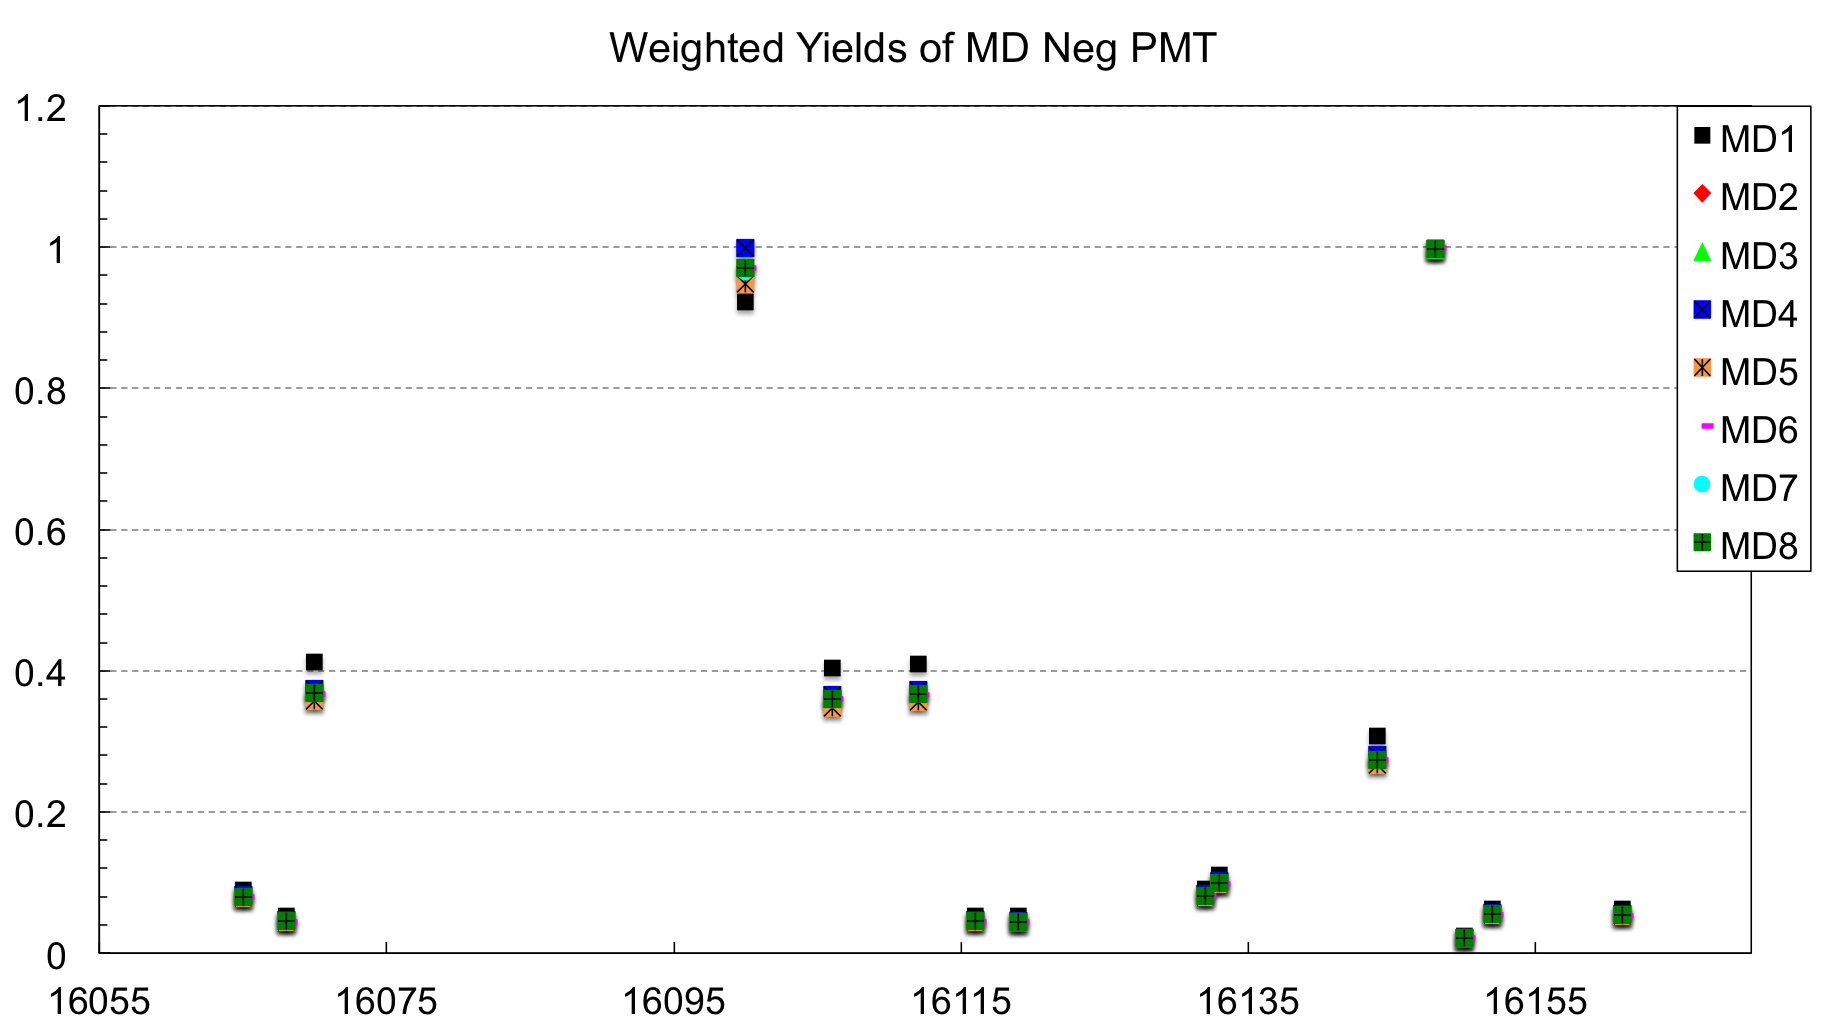
\includegraphics[width=15.0cm]{figures/transverseN2DeltaRunByRunWeightedYieldsNegPMT_old}
	\end{center}
	\caption
%	[Transverse N$\rightarrow\Delta$ run by run old weighted yields for negative PMT.]	
	{Transverse N$\rightarrow\Delta$ run by run old weighted yields for negative PMT.}
	\label{fig:transverseN2DeltaRunByRunWeightedYieldsNegPMT_old}
\end{figure}

\begin{figure}[!h]
	\begin{center}
	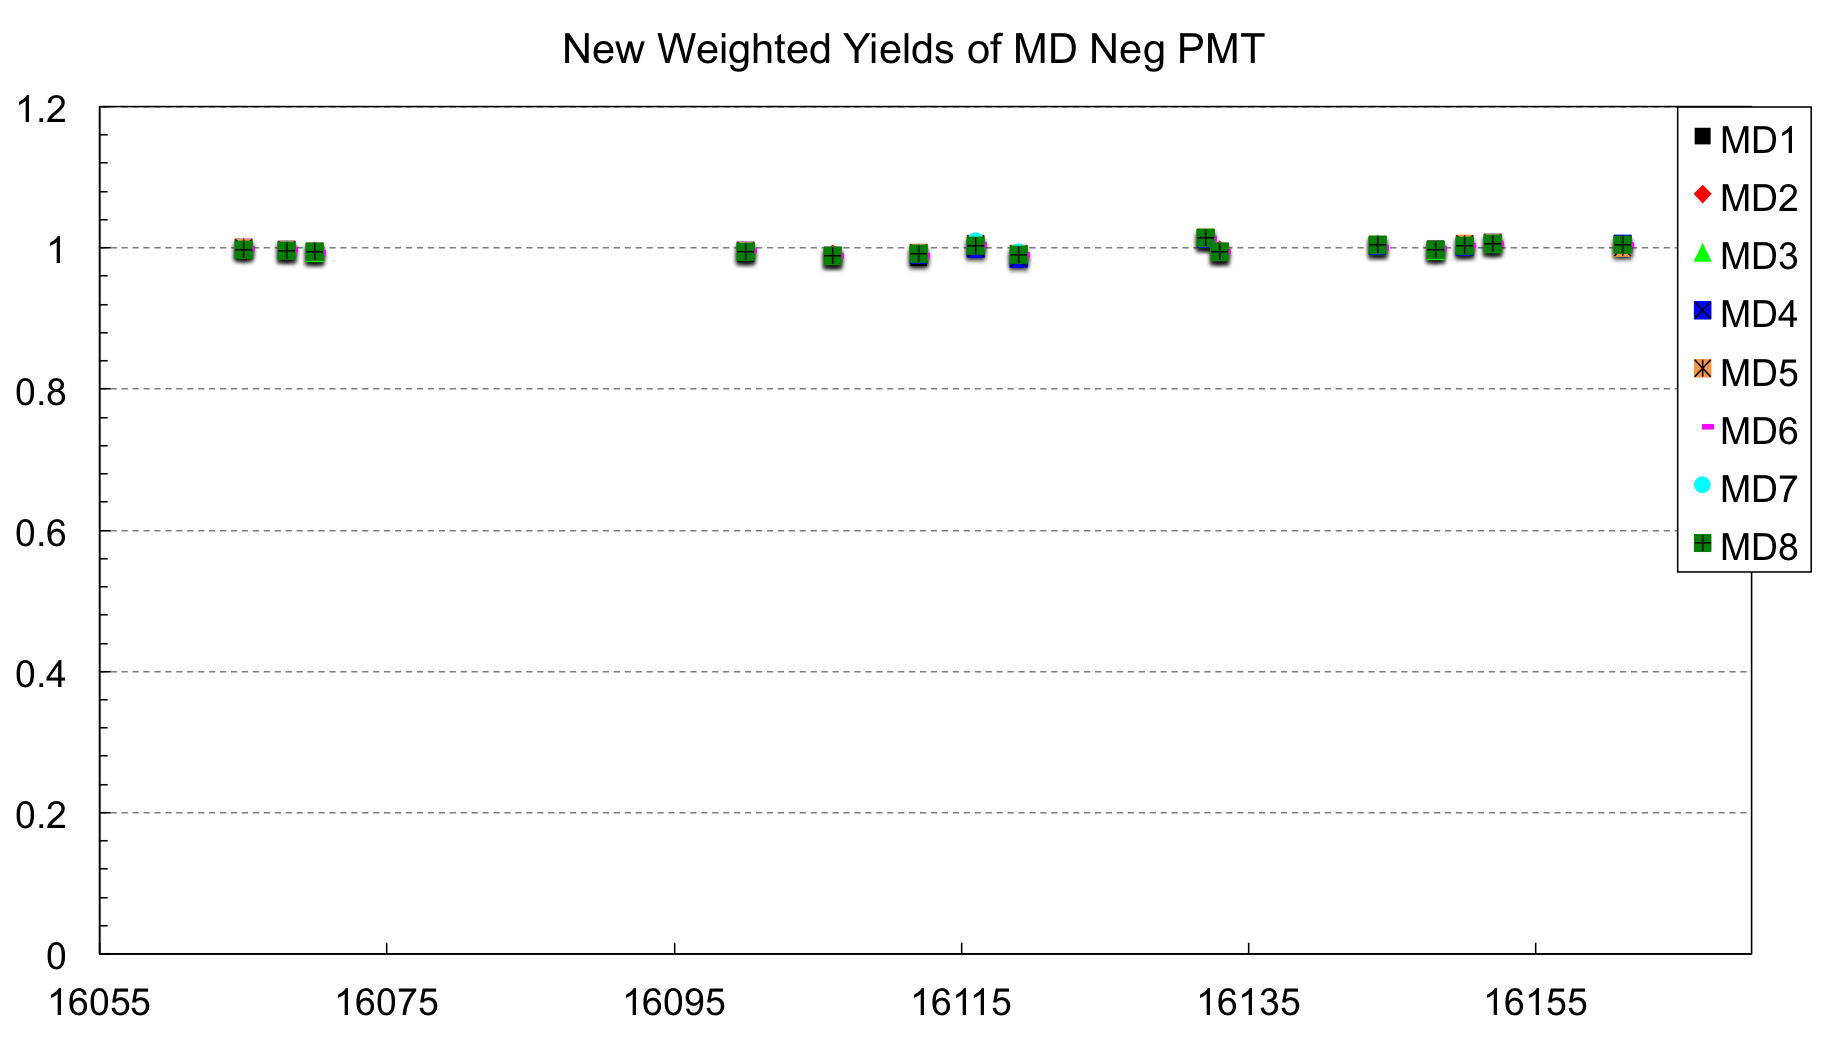
\includegraphics[width=15.0cm]{figures/transverseN2DeltaRunByRunWeightedYieldsNegPMT_UnZoomed}
	\end{center}
	\caption
%	[Transverse N$\rightarrow\Delta$ run by run new weighted yields for negative PMT.]	
	{Transverse N$\rightarrow\Delta$ run by run new weighted yields for negative PMT.}
	\label{fig:transverseN2DeltaRunByRunWeightedYieldsNegPMT_UnZoomed}
\end{figure}

\begin{figure}[!h]
	\begin{center}
	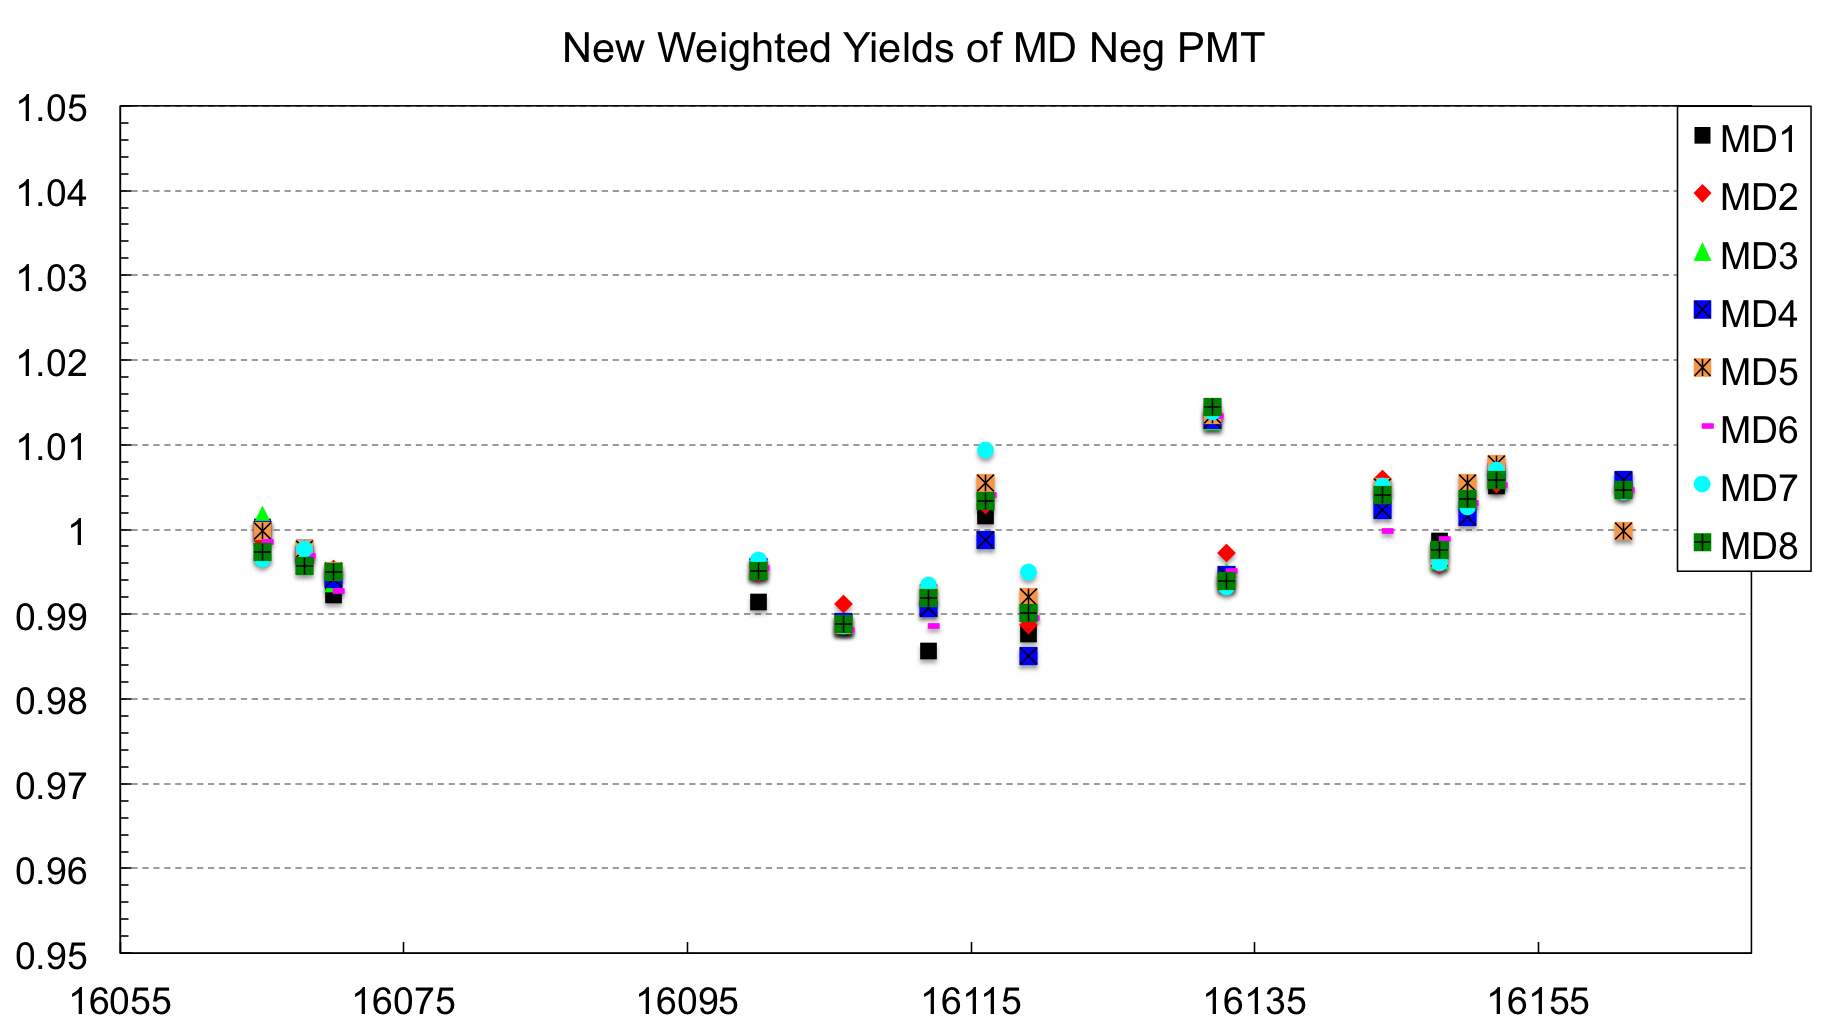
\includegraphics[width=15.0cm]{figures/transverseN2DeltaRunByRunWeightedYieldsNegPMT}
	\end{center}
	\caption
%	[Transverse N$\rightarrow\Delta$ run by run new weighted yields for negative PMT, zoomed view.]	
	{Transverse N$\rightarrow\Delta$ run by run new weighted yields for negative PMT with a zoomed view.}
	\label{fig:transverseN2DeltaRunByRunWeightedYieldsNegPMT}
\end{figure}

\begin{figure}[!h]
	\begin{center}
	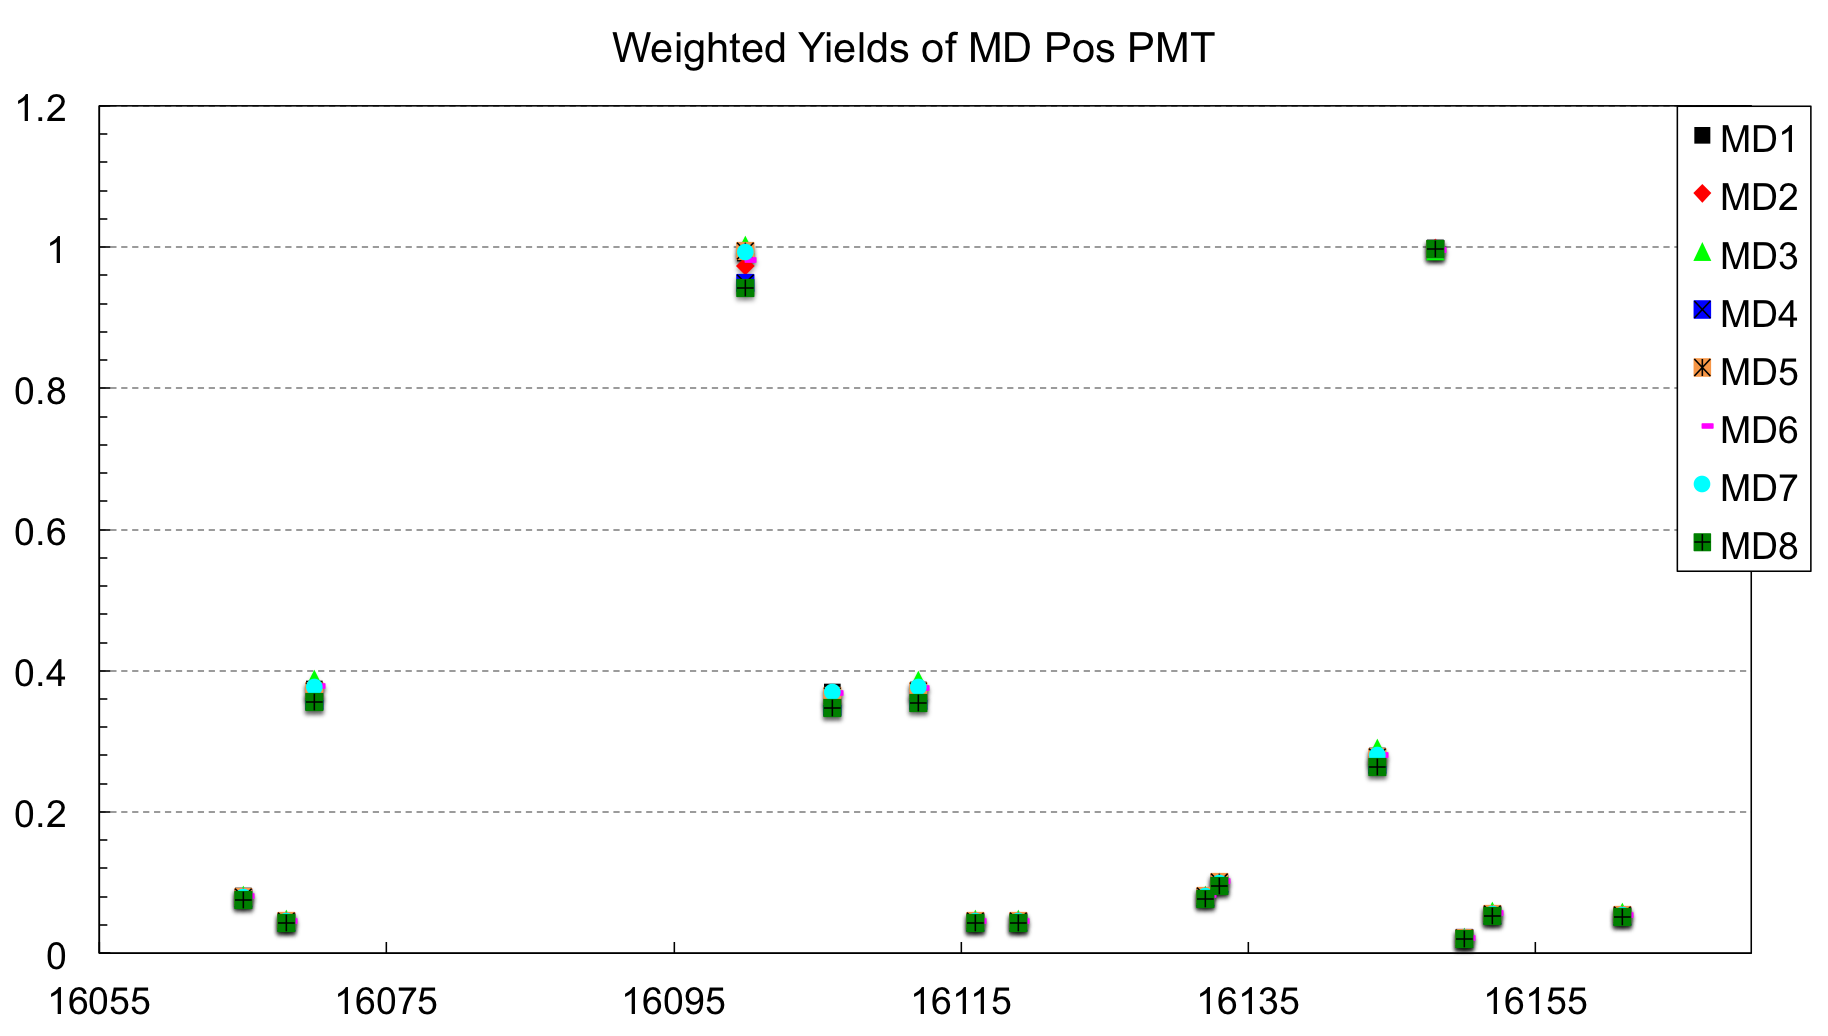
\includegraphics[width=15.0cm]{figures/transverseN2DeltaRunByRunWeightedYieldsPosPMT_old}
	\end{center}
	\caption
%	[Transverse N$\rightarrow\Delta$ run by run old weighted yields for positive PMT.]	
	{Transverse N$\rightarrow\Delta$ run by run old weighted yields for positive PMT.}
	\label{fig:transverseN2DeltaRunByRunWeightedYieldsPosPMT_old}
\end{figure}

\begin{figure}[!h]
	\begin{center}
	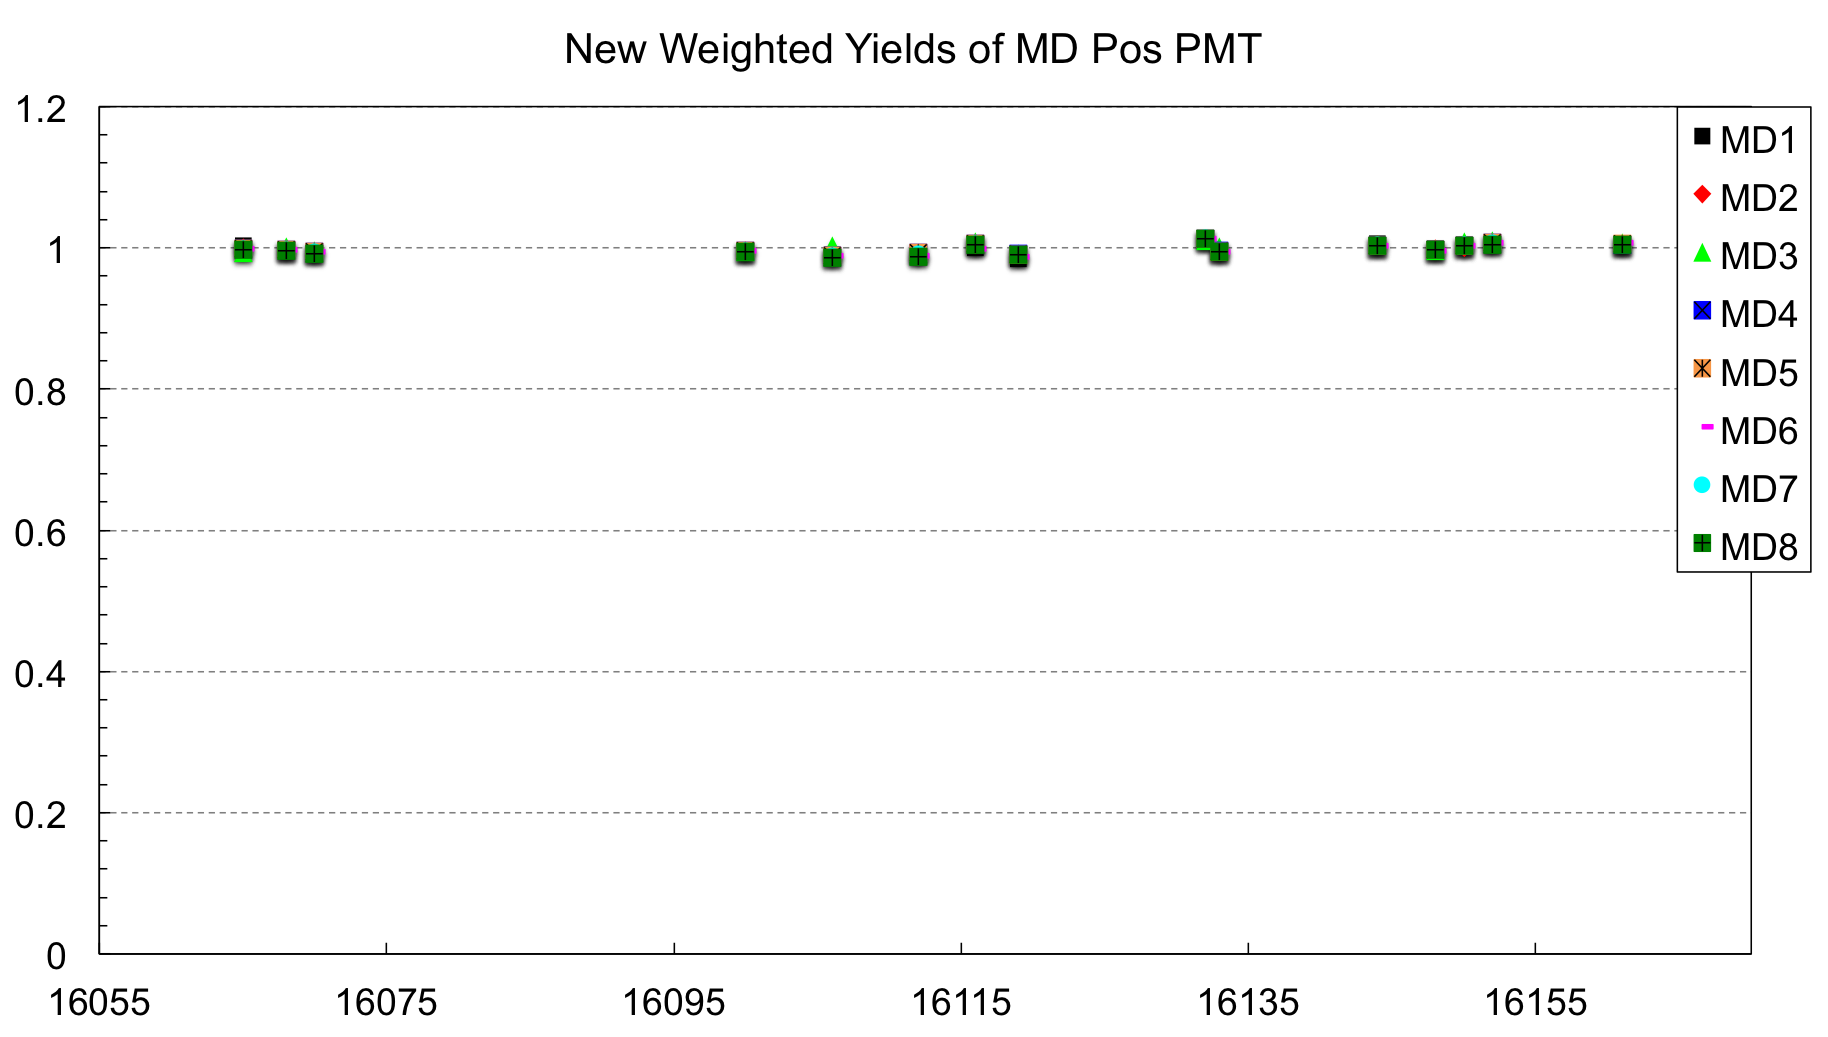
\includegraphics[width=15.0cm]{figures/transverseN2DeltaRunByRunWeightedYieldsPosPMT_UnZoomed}
	\end{center}
	\caption
%	[Transverse N$\rightarrow\Delta$ run by run new weighted yields for positive PMT.]	
	{Transverse N$\rightarrow\Delta$ run by run new weighted yields for positive PMT.}
	\label{fig:transverseN2DeltaRunByRunWeightedYieldsPosPMT_UnZoomed}
\end{figure}

\begin{figure}[!h]
	\begin{center}
	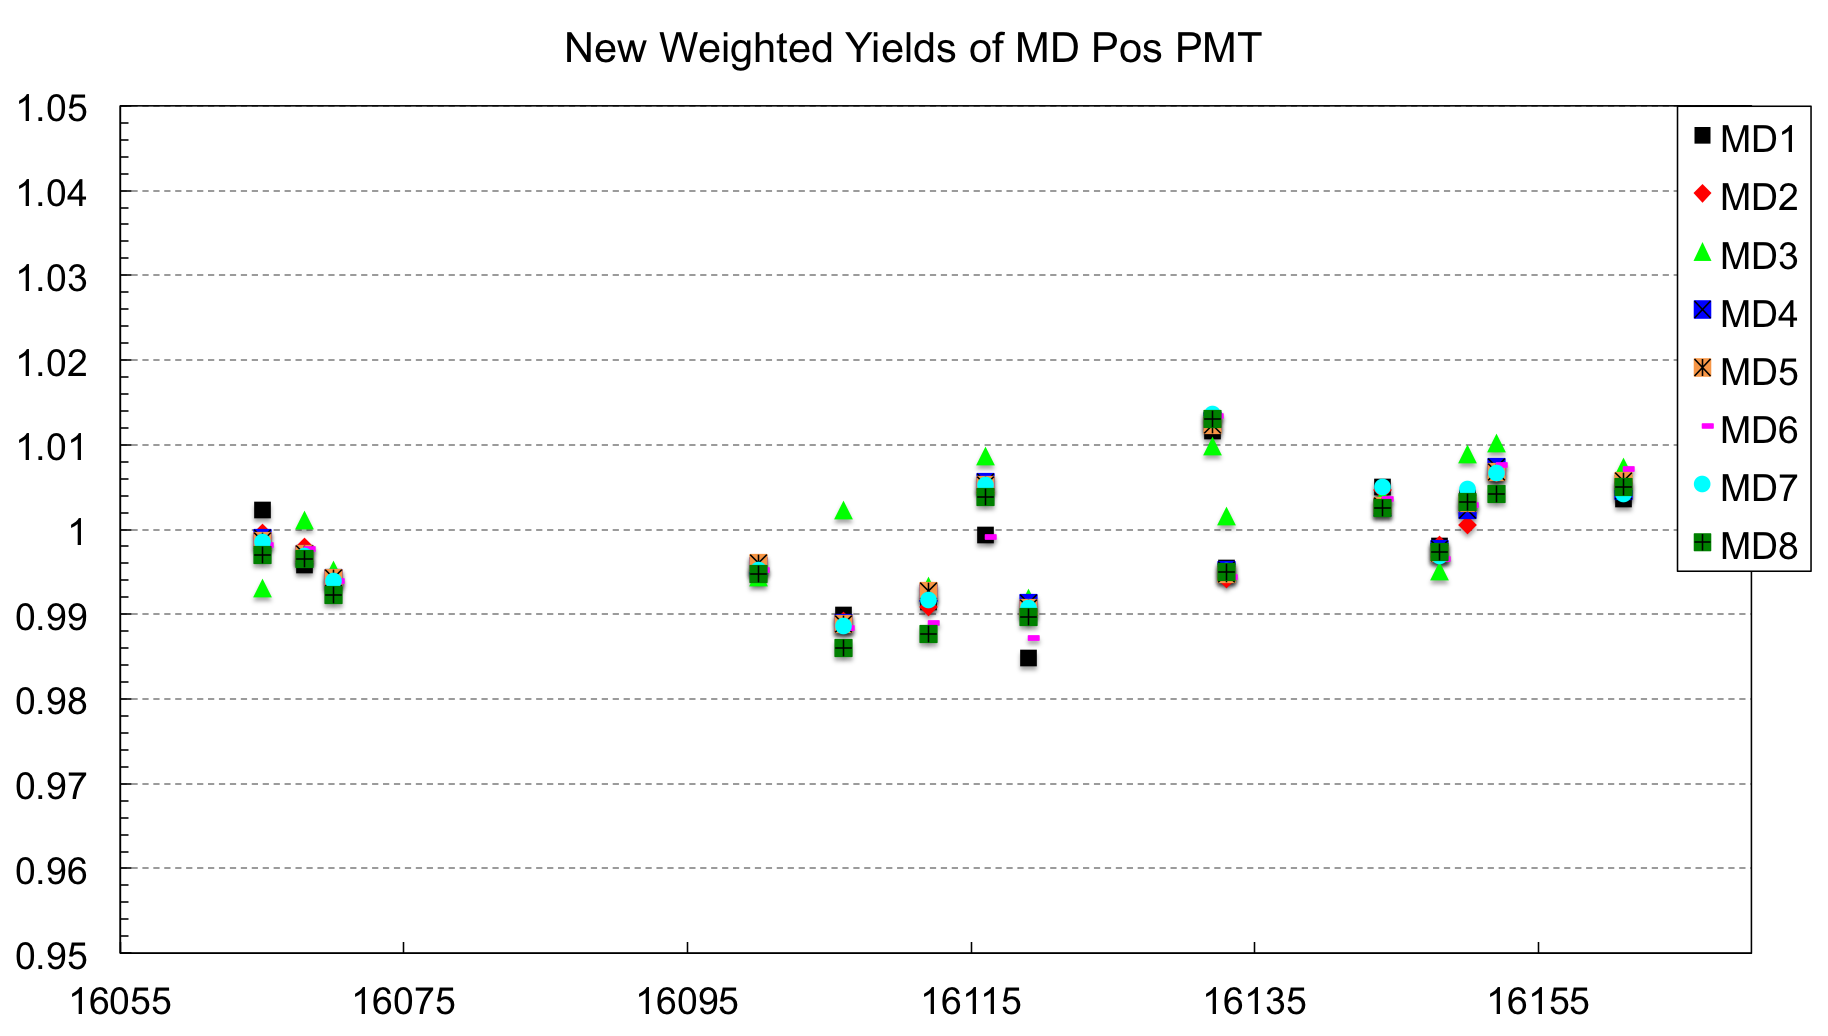
\includegraphics[width=15.0cm]{figures/transverseN2DeltaRunByRunWeightedYieldsPosPMT}
	\end{center}
	\caption
%	[Transverse N$\rightarrow\Delta$ run by run new weighted yields for positive PMT, zoomed view.]	
	{Transverse N$\rightarrow\Delta$ run by run new weighted yields for positive PMT with a zoomed view.}
	\label{fig:transverseN2DeltaRunByRunWeightedYieldsPosPMT}
\end{figure}

%transverseN2DeltaRunByRunWeightedYieldsNegPMT_old.png
%transverseN2DeltaRunByRunWeightedYieldsNegPMT_UnZoomed.png
%transverseN2DeltaRunByRunWeightedYieldsNegPMT.png
%transverseN2DeltaRunByRunWeightedYieldsPosPMT_old.png
%transverseN2DeltaRunByRunWeightedYieldsPosPMT_UnZoomed.png
%transverseN2DeltaRunByRunWeightedYieldsPosPMT.png


New weights for Run 2 transverse N$\rightarrow\Delta$ were calculated to better match the PMT gains of the main detectors~\cite{elog:buddhini_analysis800}.

Inelastic (N$\rightarrow\Delta$) hydrogen : new weights for range 16065-16066 from run 16065. Used in map file qweak\_maindet.16065-16066.map


%\begin{alltt}
%\rmfamily
% detector   	yield	inverse yield
% qwk\_md1neg 	0.0030	330.5330
% qwk\_md1pos 	0.0031	321.5347
% qwk\_md2neg 	0.0022	445.5271
% qwk\_md2pos 	0.0036	279.2840
% qwk\_md3neg 	0.0035	287.5661
% qwk\_md3pos 	0.0019	516.7349
% qwk\_md4neg 	0.0021	483.8969
% qwk\_md4pos 	0.0030	336.5697
% qwk\_md5neg 	0.0028	356.8381
% qwk\_md5pos 	0.0036	275.7896
% qwk\_md6neg 	0.0031	325.2310
% qwk\_md6pos 	0.0027	375.7575
% qwk\_md7neg 	0.0025	397.9348
% qwk\_md7pos 	0.0030	333.9648
% qwk\_md8neg 	0.0032	314.0859
% qwk\_md8pos 	0.0033	298.7560
% qwk\_md9neg 	saturating	
% qwk\_md9pos 	0.0227	 43.9706
%\end{alltt}

\clearpage

\begin{table}[!h]
\begin{center}
  	\caption
%  	[Inelastic N$\rightarrow\Delta$ hydrogen weights for range 16065-16066.]
  	{Inelastic N$\rightarrow\Delta$ hydrogen: new weights for range 16065-16066 from run 16065. Used in map file qweak\_maindet.16065-16066.map.}
  \begin{tabular}{ l | c | c }
    \noalign{\hrule height 1pt}
    Detector &	Yield	&	Inverse Yield \\ 
    \noalign{\hrule height 1pt}
 qwk\_md1neg 	& 	0.0030	&	330.5330 \\
 qwk\_md1pos 	& 	0.0031	&	321.5347 \\
 qwk\_md2neg 	& 	0.0022	&	445.5271 \\
 qwk\_md2pos 	& 	0.0036	&	279.2840 \\
 qwk\_md3neg 	& 	0.0035	&	287.5661 \\
 qwk\_md3pos 	& 	0.0019	&	516.7349 \\
 qwk\_md4neg 	& 	0.0021	&	483.8969 \\
 qwk\_md4pos 	& 	0.0030	&	336.5697 \\
 qwk\_md5neg 	& 	0.0028	&	356.8381 \\
 qwk\_md5pos 	& 	0.0036	&	275.7896 \\
 qwk\_md6neg 	& 	0.0031	&	325.2310 \\
 qwk\_md6pos 	& 	0.0027	&	375.7575 \\
 qwk\_md7neg 	& 	0.0025	&	397.9348 \\
 qwk\_md7pos 	& 	0.0030	&	333.9648 \\
 qwk\_md8neg 	& 	0.0032	&	314.0859 \\
 qwk\_md8pos 	& 	0.0033	&	298.7560 \\
 qwk\_md9neg 	&	saturating	&	 \\
 qwk\_md9pos 	& 	0.0227	&	 43.9706 \\
    \noalign{\hrule height 1pt}
  	\end{tabular}
  \label{tab:yields1}
\end{center}
\end{table}



\begin{table}[!h]
\begin{center}
  	\caption
%  	[Inelastic N$\rightarrow\Delta$ hydrogen weights for range 16129-16132.]
  	{Inelastic N$\rightarrow\Delta$ hydrogen: new weights for range 16129-16132 from run 16132. Used in map file qweak\_maindet.16129-16132.map.}
  \begin{tabular}{ l | c | c }
    \noalign{\hrule height 1pt}
    Detector &	Yield	&	Inverse Yield \\ 
    \noalign{\hrule height 1pt}
 qwk\_md1neg 	&	0.0030	&	331.4473 \\ 
 qwk\_md1pos 	&	0.0031	&	322.9721 \\ 
 qwk\_md2neg 	&	0.0022	&	444.7867 \\ 
 qwk\_md2pos 	&	0.0036	&	279.1371 \\ 
 qwk\_md3neg 	&	0.0035	&	286.4275 \\ 
 qwk\_md3pos 	&	0.0019	&	523.1008 \\ 
 qwk\_md4neg 	&	0.0021	&	484.0794 \\ 
 qwk\_md4pos 	&	0.0030	&	335.8389 \\ 
 qwk\_md5neg 	&	0.0028	&	356.5254 \\ 
 qwk\_md5pos 	&	0.0036	&	275.1948 \\ 
 qwk\_md6neg 	&	0.0031	&	324.6119 \\ 
 qwk\_md6pos 	&	0.0027	&	375.2064 \\ 
 qwk\_md7neg 	&	0.0025	&	396.6083 \\ 
 qwk\_md7pos 	&	0.0030	&	333.4368 \\ 
 qwk\_md8neg 	&	0.0032	&	313.4542 \\ 
 qwk\_md8pos 	&	0.0034	&	298.3221 \\ 
 qwk\_md8pos 	&	0.0034	&	297.3187 \\ 
 qwk\_md9neg	&	saturating	&	 \\ 
 qwk\_md9pos 	&	0.0228	&	 43.9544 \\ 
    \noalign{\hrule height 1pt}
  	\end{tabular}
  \label{tab:yields2}
\end{center}
\end{table}



\begin{table}[!h]
\begin{center}
  	\caption
%  	[Inelastic N$\rightarrow\Delta$ hydrogen weights for range 16133-16137.]
  	{Inelastic N$\rightarrow\Delta$ hydrogen: new weights for range 16133-16137 from run 16135. Used in map file qweak\_maindet.16133-16137.map.}
  \begin{tabular}{ l | c | c }
    \noalign{\hrule height 1pt}
    Detector &	Yield	&	Inverse Yield \\ 
    \noalign{\hrule height 1pt}
 qwk\_md1neg 	&	0.0038	&	266.1529 \\ 
 qwk\_md1pos 	&	0.0039	&	258.2914 \\ 
 qwk\_md2neg 	&	0.0028	&	355.5812 \\ 
 qwk\_md2pos 	&	0.0045	&	222.2689 \\ 
 qwk\_md3neg 	&	0.0044	&	228.4396 \\ 
 qwk\_md3pos 	&	0.0024	&	424.9694 \\ 
 qwk\_md4neg 	&	0.0026	&	386.2623 \\ 
 qwk\_md4pos 	&	0.0037	&	268.6043 \\ 
 qwk\_md5neg 	&	0.0035	&	284.2996 \\ 
 qwk\_md5pos 	&	0.0046	&	219.4513 \\ 
 qwk\_md6neg 	&	0.0039	&	259.7001 \\ 
 qwk\_md6pos 	&	0.0033	&	300.1012 \\ 
 qwk\_md7neg 	&	0.0032	&	316.8244 \\ 
 qwk\_md7pos 	&	0.0038	&	266.0677 \\ 
 qwk\_md8neg 	&	0.0040	&	249.5169 \\ 
 qwk\_md8pos 	&	0.0042	&	237.6253 \\ 
 qwk\_md9neg		&	0.3794	&	  2.6358 \\ 
 qwk\_md9pos 	&	0.0887	&	 11.2772 \\ 
    \noalign{\hrule height 1pt}
  	\end{tabular}
  \label{tab:yields3}
\end{center}
\end{table}

\clearpage

\begin{table}[!h]
\begin{center}
  	\caption
%  	[Inelastic N$\rightarrow\Delta$ hydrogen weights for range 16152-16158.]
  	{Inelastic N$\rightarrow\Delta$ hydrogen: new weights for range 16152-16158, from run 16152. Used in map file qweak\_maindet.16152-16158.map.}
  \begin{tabular}{ l | c | c }
    \noalign{\hrule height 1pt}
    Detector &	Yield	&	Inverse Yield \\ 
    \noalign{\hrule height 1pt}
 qwk\_md1neg 	&	0.0021	&	477.6794 \\ 
 qwk\_md1pos 	&	0.0021	&	472.5407 \\ 
 qwk\_md2neg 	&	0.0016	&	644.8716 \\ 
 qwk\_md2pos 	&	0.0025	&	404.0438 \\ 
 qwk\_md3neg 	&	0.0024	&	415.0359 \\ 
 qwk\_md3pos 	&	0.0014	&	728.0065 \\ 
 qwk\_md4neg 	&	0.0014	&	704.6771 \\ 
 qwk\_md4pos 	&	0.0021	&	487.6773 \\ 
 qwk\_md5neg 	&	0.0019	&	517.9050 \\ 
 qwk\_md5pos 	&	0.0025	&	401.9060 \\ 
 qwk\_md6neg 	&	0.0021	&	474.0913 \\ 
 qwk\_md6pos 	&	0.0018	&	546.7656 \\ 
 qwk\_md7neg 	&	0.0017	&	576.2694 \\ 
 qwk\_md7pos 	&	0.0021	&	486.3954 \\ 
 qwk\_md8neg 	&	0.0022	&	456.6464 \\ 
 qwk\_md8pos 	&	0.0023	&	435.2565 \\ 
 qwk\_md9neg 	&	0.0498	&	 20.0761 \\ 
 qwk\_md9pos 	&	0.0122	&	 81.7203 \\ 
    \noalign{\hrule height 1pt}
  	\end{tabular}
  \label{tab:yields4}
\end{center}
\end{table}


\begin{table}[!h]
\begin{center}
  	\caption
%  	[Inelastic N$\rightarrow\Delta$ aluminum weights for range 16067-16069.]
  	{Inelastic N$\rightarrow\Delta$ aluminum: new weights for ranges 16067-16069 and 16115-16124 from run 16067. Used in map files qweak\_maindet.16067-16069.map and qweak\_maindet.16115-16124.map.}
  \begin{tabular}{ l | c | c }
    \noalign{\hrule height 1pt}
    Detector &	Yield	&	Inverse Yield \\ 
    \noalign{\hrule height 1pt}
 qwk\_md1neg 	&	0.0018	&	563.1134 \\ 
 qwk\_md1pos 	&	0.0018	&	567.0229 \\ 
 qwk\_md2neg 	&	0.0013	&	791.2187 \\ 
 qwk\_md2pos 	&	0.0020	&	494.0402 \\ 
 qwk\_md3neg 	&	0.0020	&	508.6698 \\ 
 qwk\_md3pos 	&	0.0011	&	887.0735 \\ 
 qwk\_md4neg 	&	0.0012	&	854.3876 \\ 
 qwk\_md4pos 	&	0.0017	&	595.1733 \\ 
 qwk\_md5neg 	&	0.0016	&	632.2300 \\ 
 qwk\_md5pos 	&	0.0020	&	488.4802 \\ 
 qwk\_md6neg 	&	0.0017	&	577.2902 \\ 
 qwk\_md6pos 	&	0.0015	&	662.4486 \\ 
 qwk\_md7neg 	&	0.0014	&	691.0762 \\ 
 qwk\_md7pos 	&	0.0017	&	582.1006 \\ 
 qwk\_md8neg 	&	0.0018	&	552.0701 \\ 
 qwk\_md8pos 	&	0.0019	&	528.0746 \\ 
 qwk\_md9neg 	&	saturating	&	 \\ 
 qwk\_md9pos 	&	0.0114	&	 87.7754 \\ 
    \noalign{\hrule height 1pt}
  	\end{tabular}
  \label{tab:yields5}
\end{center}
\end{table}


\begin{table}[!h]
\begin{center}
  	\caption
%  	[Inelastic N$\rightarrow\Delta$ aluminum weights for range 16160-16161.]
  	{Inelastic N$\rightarrow\Delta$ aluminum: new weights for range 16160-16161, from run 16160. Used in map file qweak\_maindet.16160-16161.map.}
  \begin{tabular}{ l | c | c }
    \noalign{\hrule height 1pt}
    Detector &	Yield	&	Inverse Yield \\ 
    \noalign{\hrule height 1pt}
 qwk\_md1neg 	&	0.0021	&	476.9109 \\ 
 qwk\_md1pos 	&	0.0021	&	474.5462 \\ 
 qwk\_md2neg 	&	0.0015	&	665.1318 \\ 
 qwk\_md2pos 	&	0.0024	&	415.4953 \\ 
 qwk\_md3neg 	&	0.0023	&	428.0483 \\ 
 qwk\_md3pos 	&	0.0013	&	746.6703 \\ 
 qwk\_md4neg 	&	0.0014	&	723.3967 \\ 
 qwk\_md4pos 	&	0.0020	&	501.2203 \\ 
 qwk\_md5neg 	&	0.0019	&	530.5362 \\ 
 qwk\_md5pos 	&	0.0024	&	411.7435 \\ 
 qwk\_md6neg 	&	0.0021	&	487.6173 \\ 
 qwk\_md6pos 	&	0.0018	&	565.3161 \\ 
 qwk\_md7neg 	&	0.0017	&	582.9472 \\ 
 qwk\_md7pos 	&	0.0020	&	489.5450 \\ 
 qwk\_md8neg 	&	0.0022	&	464.5394 \\ 
 qwk\_md8pos 	&	0.0022	&	444.8808 \\ 
 qwk\_md9neg 	&	0.1340	&	  7.4654 \\ 
 qwk\_md9pos 	&	0.0322	&	 31.0311 \\ 
    \noalign{\hrule height 1pt}
  	\end{tabular}
  \label{tab:yields6}
\end{center}
\end{table}


\begin{table}[!h]
\begin{center}
  	\caption
%  	[Inelastic N$\rightarrow\Delta$ carbon weights for range 16148-16151.]
  	{Inelastic N$\rightarrow\Delta$ carbon: new weights for range 16148-16151, from run 16148.Used in map file qweak\_maindet.16148-16151.map.}
  \begin{tabular}{ l | c | c }
    \noalign{\hrule height 1pt}
    Detector &	Yield	&	Inverse Yield \\ 
    \noalign{\hrule height 1pt}
 qwk\_md1neg 	&	0.0008	&	1205.9293 \\ 
 qwk\_md1pos 	&	0.0008	&	1216.4200 \\ 
 qwk\_md2neg 	&	0.0006	&	1681.8313 \\ 
 qwk\_md2pos 	&	0.0010	&	1050.1477 \\ 
 qwk\_md3neg 	&	0.0009	&	1081.4484 \\ 
 qwk\_md3pos 	&	0.0005	&	1888.8651 \\ 
 qwk\_md4neg 	&	0.0005	&	1818.8889 \\ 
 qwk\_md4pos 	&	0.0008	&	1251.2483 \\ 
 qwk\_md5neg 	&	0.0007	&	1343.7638 \\ 
 qwk\_md5pos 	&	0.0010	&	1039.5739 \\ 
 qwk\_md6neg 	&	0.0008	&	1219.9163 \\ 
 qwk\_md6pos 	&	0.0007	&	1415.7069 \\ 
 qwk\_md7neg 	&	0.0007	&	1473.6067 \\ 
 qwk\_md7pos 	&	0.0008	&	1250.6393 \\ 
 qwk\_md8neg 	&	0.0008	&	1183.1535 \\ 
 qwk\_md8pos 	&	0.0009	&	1127.1379 \\ 
 qwk\_md9neg 	&	0.0310	&	  32.2814 \\ 
 qwk\_md9pos 	&	0.0071	&	 141.5792 \\ 
    \noalign{\hrule height 1pt}
  	\end{tabular}
  \label{tab:yields7}
\end{center}
\end{table}



A brief weighted yield and relative weighted yield for the entire parity-violating production dataset are shown in Figure~\ref{fig:qweakPVweightedYield} and Figure~\ref{fig:qweakPVrelWeightedYield} (APPENDIX~\ref{Miscellaneous}).







% qwk_md1neg 	0.0030	330.5330
% qwk_md1pos 	0.0031	321.5347
% qwk_md2neg 	0.0022	445.5271
% qwk_md2pos 	0.0036	279.2840
% qwk_md3neg 	0.0035	287.5661
% qwk_md3pos 	0.0019	516.7349
% qwk_md4neg 	0.0021	483.8969
% qwk_md4pos 	0.0030	336.5697
% qwk_md5neg 	0.0028	356.8381
% qwk_md5pos 	0.0036	275.7896
% qwk_md6neg 	0.0031	325.2310
% qwk_md6pos 	0.0027	375.7575
% qwk_md7neg 	0.0025	397.9348
% qwk_md7pos 	0.0030	333.9648
% qwk_md8neg 	0.0032	314.0859
% qwk_md8pos 	0.0033	298.7560
% qwk_md9neg 	saturating	
% qwk_md9pos 	0.0227	 43.9706
%
%
%Since md9neg was saturating for this whole range, for the sake of adding a weight to the map file, I used the observed relative weights from previous runs (16058-16096) as dummy weights.
%These relative weights are: md9neg = 0.24, md9pos = 0.76. Anyway these will be useless since we cannot create barsums with a single PMT. 
%
%
%
%Inelastic (N->Delta) hydrogen : new weights for range 16129-16132 from run 16132. Used in map file qweak_maindet.16129-16132.map
%
% qwk_md1neg 	0.0030	331.4473
% qwk_md1pos 	0.0031	322.9721
% qwk_md2neg 	0.0022	444.7867
% qwk_md2pos 	0.0036	279.1371
% qwk_md3neg 	0.0035	286.4275
% qwk_md3pos 	0.0019	523.1008
% qwk_md4neg 	0.0021	484.0794
% qwk_md4pos 	0.0030	335.8389
% qwk_md5neg 	0.0028	356.5254
% qwk_md5pos 	0.0036	275.1948
% qwk_md6neg 	0.0031	324.6119
% qwk_md6pos 	0.0027	375.2064
% qwk_md7neg 	0.0025	396.6083
% qwk_md7pos 	0.0030	333.4368
% qwk_md8neg 	0.0032	313.4542
% qwk_md8pos 	0.0034	298.3221
% qwk_md8pos 	0.0034	297.3187
% qwk_md9neg	saturating	
% qwk_md9pos 	0.0228	 43.9544
%
%Since md9neg was saturating for this whole range, I used the observed relative weights from run 16135 as dummy weights.
%From run 16135, relative weights of md9neg and md9pos are 0.19 and 0.81. Anyway these will be useless since we cannot create barsums with a single PMT. 
%
%
%
%Inelastic (N->Delta) hydrogen : new weights for range 16133-16137 from run 16135. Used in map file qweak_maindet.16133-16137.map
%
% detector   	yield	inverse yield
% qwk_md1neg 	0.0038	266.1529
% qwk_md1pos 	0.0039	258.2914
% qwk_md2neg 	0.0028	355.5812
% qwk_md2pos 	0.0045	222.2689
% qwk_md3neg 	0.0044	228.4396
% qwk_md3pos 	0.0024	424.9694
% qwk_md4neg 	0.0026	386.2623
% qwk_md4pos 	0.0037	268.6043
% qwk_md5neg 	0.0035	284.2996
% qwk_md5pos 	0.0046	219.4513
% qwk_md6neg 	0.0039	259.7001
% qwk_md6pos 	0.0033	300.1012
% qwk_md7neg 	0.0032	316.8244
% qwk_md7pos 	0.0038	266.0677
% qwk_md8neg 	0.0040	249.5169
% qwk_md8pos 	0.0042	237.6253
% qwk_md9neg	0.3794	  2.6358
% qwk_md9pos 	0.0887	 11.2772
%
%
%
%
%
%Inelastic (N->Delta) hydrogen : new weights for range 16152-16158, from run 16152. Used in map file qweak_maindet.16152-16158.map
%
% detector	yield	inverse yield
% qwk_md1neg 	0.0021	477.6794
% qwk_md1pos 	0.0021	472.5407
% qwk_md2neg 	0.0016	644.8716
% qwk_md2pos 	0.0025	404.0438
% qwk_md3neg 	0.0024	415.0359
% qwk_md3pos 	0.0014	728.0065
% qwk_md4neg 	0.0014	704.6771
% qwk_md4pos 	0.0021	487.6773
% qwk_md5neg 	0.0019	517.9050
% qwk_md5pos 	0.0025	401.9060
% qwk_md6neg 	0.0021	474.0913
% qwk_md6pos 	0.0018	546.7656
% qwk_md7neg 	0.0017	576.2694
% qwk_md7pos 	0.0021	486.3954
% qwk_md8neg 	0.0022	456.6464
% qwk_md8pos 	0.0023	435.2565
% qwk_md9neg 	0.0498	 20.0761
% qwk_md9pos 	0.0122	 81.7203
%
%
%
%
%Inelastic (N->Delta) aluminum : new weights for ranges 16067-16069 and 16115-16124 from run 16067. Used in map files qweak_maindet.16067-16069.map and qweak_maindet.16115-16124.map
%
%
% detector   	yield	inverse yield
% qwk_md1neg 	0.0018	563.1134
% qwk_md1pos 	0.0018	567.0229
% qwk_md2neg 	0.0013	791.2187
% qwk_md2pos 	0.0020	494.0402
% qwk_md3neg 	0.0020	508.6698
% qwk_md3pos 	0.0011	887.0735
% qwk_md4neg 	0.0012	854.3876
% qwk_md4pos 	0.0017	595.1733
% qwk_md5neg 	0.0016	632.2300
% qwk_md5pos 	0.0020	488.4802
% qwk_md6neg 	0.0017	577.2902
% qwk_md6pos 	0.0015	662.4486
% qwk_md7neg 	0.0014	691.0762
% qwk_md7pos 	0.0017	582.1006
% qwk_md8neg 	0.0018	552.0701
% qwk_md8pos 	0.0019	528.0746
% qwk_md9neg 	saturating	
% qwk_md9pos 	0.0114	 87.7754
%
%Since md9neg was saturating for this whole range, I used the observed relative weights from previous run range (with same kinematics) as dummy weights.
%Relative weights of md9neg and md9pos are 0.23 and 0.77. Anyway these will be useless since we cannot create barsums with a single PMT. 
%
%
%
%Inelastic (N->Delta) aluminum : new weights for range 16160-16161, from run 16160. Used in map file qweak_maindet.16160-16161.map
%
%
%detector	yield	inverse yield
% qwk_md1neg 	0.0021	476.9109
% qwk_md1pos 	0.0021	474.5462
% qwk_md2neg 	0.0015	665.1318
% qwk_md2pos 	0.0024	415.4953
% qwk_md3neg 	0.0023	428.0483
% qwk_md3pos 	0.0013	746.6703
% qwk_md4neg 	0.0014	723.3967
% qwk_md4pos 	0.0020	501.2203
% qwk_md5neg 	0.0019	530.5362
% qwk_md5pos 	0.0024	411.7435
% qwk_md6neg 	0.0021	487.6173
% qwk_md6pos 	0.0018	565.3161
% qwk_md7neg 	0.0017	582.9472
% qwk_md7pos 	0.0020	489.5450
% qwk_md8neg 	0.0022	464.5394
% qwk_md8pos 	0.0022	444.8808
% qwk_md9neg 	0.1340	  7.4654
% qwk_md9pos 	0.0322	 31.0311
%
%
%
%Inelastic (N->Delta) carbon : new weights for range 16148-16151, from run 16148.Used in map file qweak_maindet.16148-16151.map
%
%detector	yield	inverse yield
% qwk_md1neg 	0.0008	1205.9293
% qwk_md1pos 	0.0008	1216.4200
% qwk_md2neg 	0.0006	1681.8313
% qwk_md2pos 	0.0010	1050.1477
% qwk_md3neg 	0.0009	1081.4484
% qwk_md3pos 	0.0005	1888.8651
% qwk_md4neg 	0.0005	1818.8889
% qwk_md4pos 	0.0008	1251.2483
% qwk_md5neg 	0.0007	1343.7638
% qwk_md5pos 	0.0010	1039.5739
% qwk_md6neg 	0.0008	1219.9163
% qwk_md6pos 	0.0007	1415.7069
% qwk_md7neg 	0.0007	1473.6067
% qwk_md7pos 	0.0008	1250.6393
% qwk_md8neg 	0.0008	1183.1535
% qwk_md8pos 	0.0009	1127.1379
% qwk_md9neg 	0.0310	  32.2814
% qwk_md9pos 	0.0071	 141.5792
%


%%%%%%%%%%%%%%%%%%%%%%%%%%%%%%%%%%%%%%%%%%%%%%%%%%%%%%%%%%%%%
\section{Uncertainty in Physics Asymmetries}
\label{Uncertainty in Physics Asymmetries}

\begin{equation} \label{equ:dPhysicsAsymmetryAmsr}
(dB_{n})_{\epsilon_{reg}} = M_{RC}M_{Det}M_{Q^{2}}M_{\phi} \frac{d\epsilon_{reg}}{P} \left[ \frac{ 1 }{1 - f_{Al} - f_{BB} - f_{QTor} - f_{el}} \right] 
\end{equation}

\begin{equation} \label{equ:dPhysicsAsymmetryP}
(dB_{n})_{P} = M_{RC}M_{Det}M_{Q^{2}}M_{\phi} \frac{\epsilon_{reg}}{P} \frac{dP}{P} \left[ \frac{ 1 }{1 - f_{Al} - f_{BB} - f_{QTor} - f_{el}} \right] 
\end{equation}

\begin{equation} \label{equ:dPhysicsAsymmetryBAl}
(dB_{n})_{B_{Al}} = M_{RC}M_{Det}M_{Q^{2}}M_{\phi} \left[ \frac{ -dB_{Al}f_{Al} }{1 - f_{Al} - f_{BB} - f_{QTor} - f_{el}} \right] 
\end{equation}

%\begin{equation} \label{equ:dPhysicsAsymmetryBBB}
%(dB_{n})_{B_{BB}} = M_{RC}M_{Det}M_{Q^{2}}M_{\phi} \left[ \frac{ -dB_{BB}f_{BB} }{1 - f_{Al} - f_{BB} - f_{QTor} - f_{el}} \right] 
%\end{equation}

\begin{equation} \label{equ:dPhysicsAsymmetryBQTor}
(dB_{n})_{B_{QTor}} = M_{RC}M_{Det}M_{Q^{2}}M_{\phi} \left[ \frac{ -dB_{QTor}f_{QTor} }{1 - f_{Al} - f_{BB} - f_{QTor} - f_{el}} \right] 
\end{equation}

\begin{equation} \label{equ:dPhysicsAsymmetryBel}
(dB_{n})_{B_{el}} = M_{RC}M_{Det}M_{Q^{2}}M_{\phi} \left[ \frac{ -dB_{el}f_{el} }{1 - f_{Al} - f_{BB} - f_{QTor} - f_{el}} \right] 
\end{equation}

\begin{equation} \label{equ:dPhysicsAsymmetryfAl}
(dB_{n})_{f_{Al}} = M_{RC}M_{Det}M_{Q^{2}}M_{\phi} df_{Al} \left[ \frac{ \frac{\epsilon_{reg}}{P} - B_{Al}(1 - f_{BB} - f_{QTor} - f_{el}) - B_{QTor}f_{QTor} - B_{el}f_{el} }{ (1 - f_{Al} - f_{BB} - f_{QTor} - f_{el})^{2} } \right] 
\end{equation}

\begin{equation} \label{equ:dPhysicsAsymmetryfBB}
(dB_{n})_{f_{BB}} = M_{RC}M_{Det}M_{Q^{2}}M_{\phi} df_{BB} \left[ \frac{ \frac{\epsilon_{reg}}{P} - B_{Al}f_{Al} - B_{QTor}f_{QTor} - B_{el}f_{el} }{ (1 - f_{Al} - f_{BB} - f_{QTor} - f_{el})^{2} } \right] 
\end{equation}

\begin{equation} \label{equ:dPhysicsAsymmetryfQTor}
(dB_{n})_{f_{QTor}} = M_{RC}M_{Det}M_{Q^{2}}M_{\phi} df_{QTor} \left[ \frac{ \frac{\epsilon_{reg}}{P} - B_{Al}f_{Al} - B_{QTor}(1 - f_{Al} - f_{BB} - f_{el}) - B_{el}f_{el} }{ (1 - f_{Al} - f_{BB} - f_{QTor} - f_{el})^{2} } \right] 
\end{equation}

\begin{equation} \label{equ:dPhysicsAsymmetryfel}
(dB_{n})_{f_{el}} = M_{RC}M_{Det}M_{Q^{2}}M_{\phi} df_{el} \left[ \frac{ \frac{\epsilon_{reg}}{P} - B_{Al}f_{Al} - B_{QTor}f_{QTor} - B_{el}(1 - f_{Al} - f_{BB} - f_{QTor}) }{ (1 - f_{Al} - f_{BB} - f_{QTor} - f_{el})^{2} } \right] 
\end{equation}

\begin{table}[!h]
\begin{center}
  	\caption
%  	[Systematic error table.]
  	{Systematic error table.}
  \begin{tabular}{ c | c | c }
%    \hline
    \noalign{\hrule height 1pt}
    \multirow{2}{*}{Error from}	&	Uncertainty	&	Relative uncertainty \\
							&	[ppm]	&	[\%] \\
%	\hline
    \noalign{\hrule height 1pt}
	$\epsilon_{reg}$	&	2.36		&	5.9 \\
	P				&	0.26		&	0.7 \\
	$B_{Al}$			&	0.17		&	0.4 \\
%	$B_{BB}$			&	0.55		&	1.4 \\
	$B_{QTor}$		&	0.02		&	0.1 \\
	$B_{el}$			&	0.47		&	1.2 \\
	$f_{Al}$			&	0.30		&	0.7 \\
	$f_{BB}$			&	0.13		&	0.3 \\
	$f_{QTor}$		&	1.70		&	4.3 \\
	$f_{el}$			&	13.96	&	35.2 \\
	$M_{RC}$			&	0.00		&	0.0 \\
	$M_{Det}$		&	0.00		&	0.0 \\
	$M_{Q^{2}}$		&	1.19		&	3.0 \\
	$M_{\phi}$		&	0.00		&	0.0 \\
%	\hline
    \noalign{\hrule height 1pt}
	Total			& 	14.33 	&	36.1 \\
%    \hline
    \noalign{\hrule height 1pt}
  	\end{tabular}
  \label{tab:PhysicsError}
\end{center}
\end{table}


%%%%%%%%%%%%%%%%%%%%%%%%%%%%%%%%%%%%%%%%%%%%%%%%%%%%%%%%%%%%%
\section{Corrections}
\label{Corrections}

\begin{figure}[!h]
	\begin{center}
	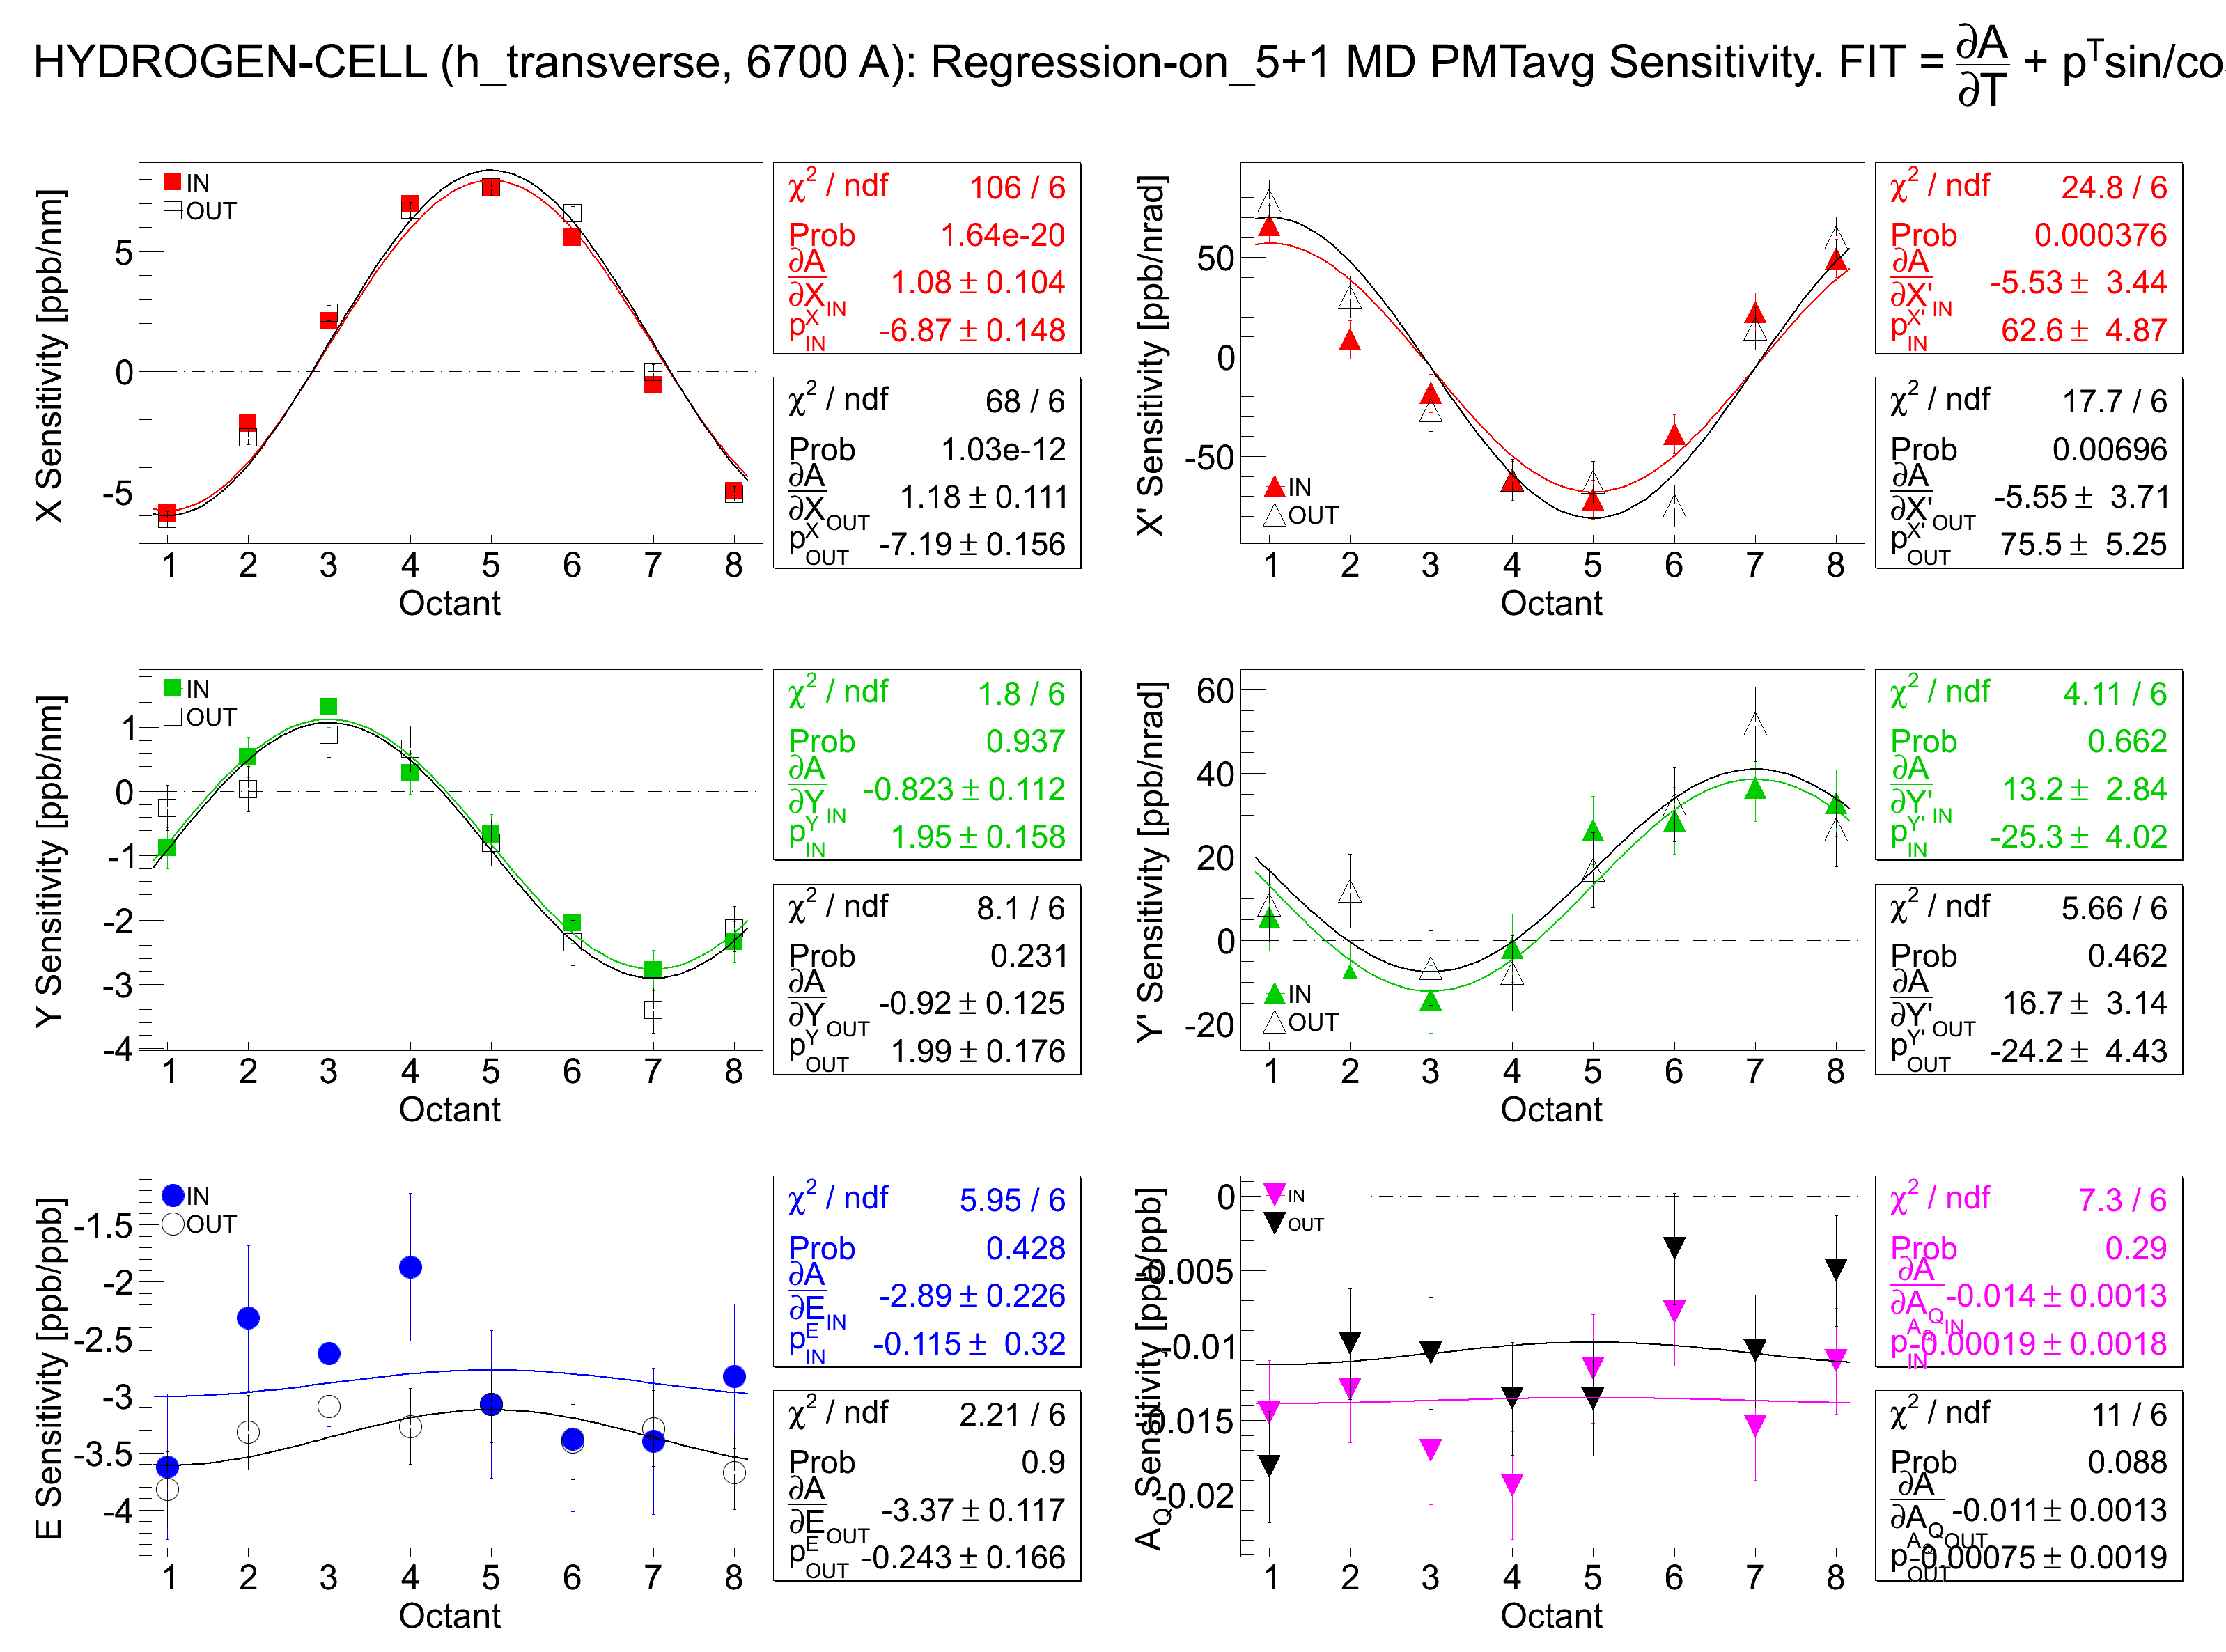
\includegraphics[width=15.0cm]{figures/MD_h_transverse_5+1_Sensitivities}
	\end{center}
	\caption
%	[Azimuthal dependence of the main detector sensitivities to HCBA in the horizontal LH$_{2}$ transverse data set.]	
	{Azimuthal dependence of the main detector sensitivities to HCBA for the ``5+1" regression scheme in the horizontal LH$_{2}$ transverse data set are shown here. Sensitivities for beam positions and angles have sinusoidal dependence with octant. No such strong dependence is seen for energy and charge. Two IHWP states are shown separately for each beam parameter. Fit functions used to fit the parameters are shown on the plot. The constant in the fit gives the error weighted average of the sensitivities.}
	\label{fig:MD_h_transverse_5+1_Sensitivities}
\end{figure}

\begin{figure}[!h]
	\begin{center}
	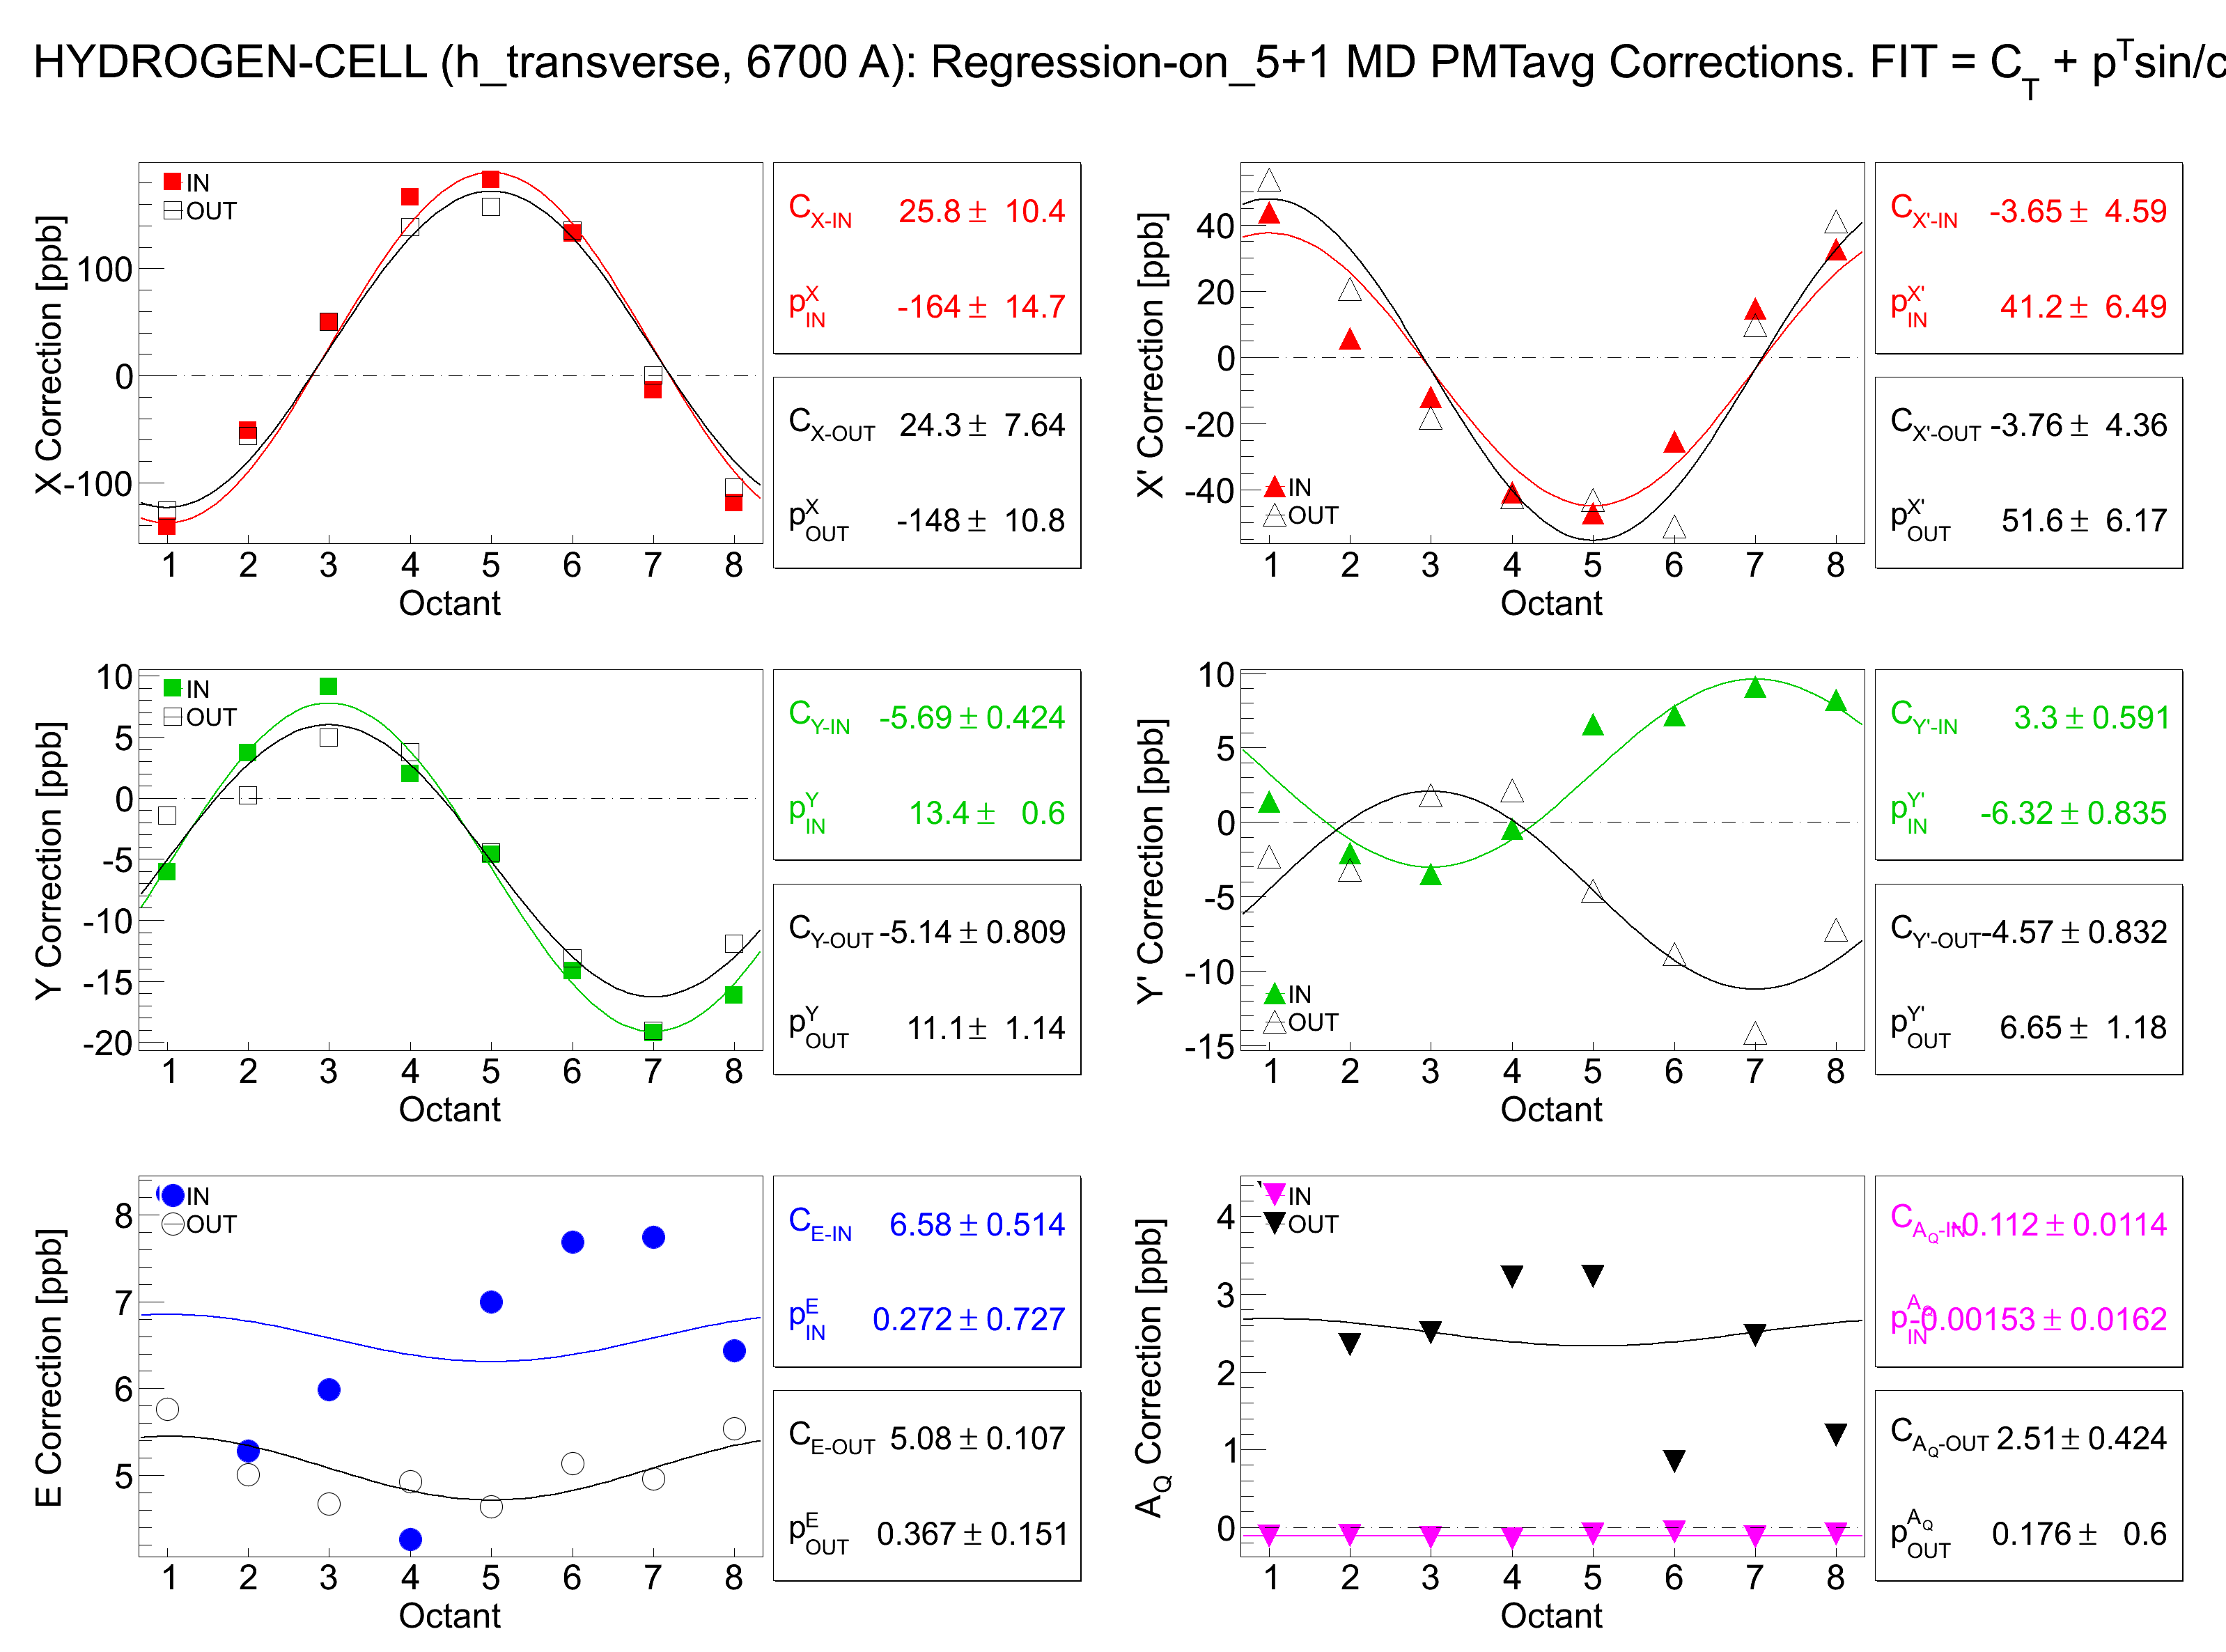
\includegraphics[width=15.0cm]{figures/MD_h_transverse_5+1_corrections}
	\end{center}
	\caption
%	[Main detector corrections vs octant for horizontal transverse data set.]	
	{Main detector corrections (using sensitivities from ``5+1" regression scheme) vs octant for horizontal LH$_{2}$ transverse data set are shown here. Beam positions and angles have sinusoidal dependence with octant inherited from the sensitivities. No such dependence is seen for energy and charge. Both IHWP states are shown separately for each beam parameter.}
	\label{fig:MD_h_transverse_5+1_corrections}
\end{figure}

\begin{figure}[!h]
	\begin{center}
	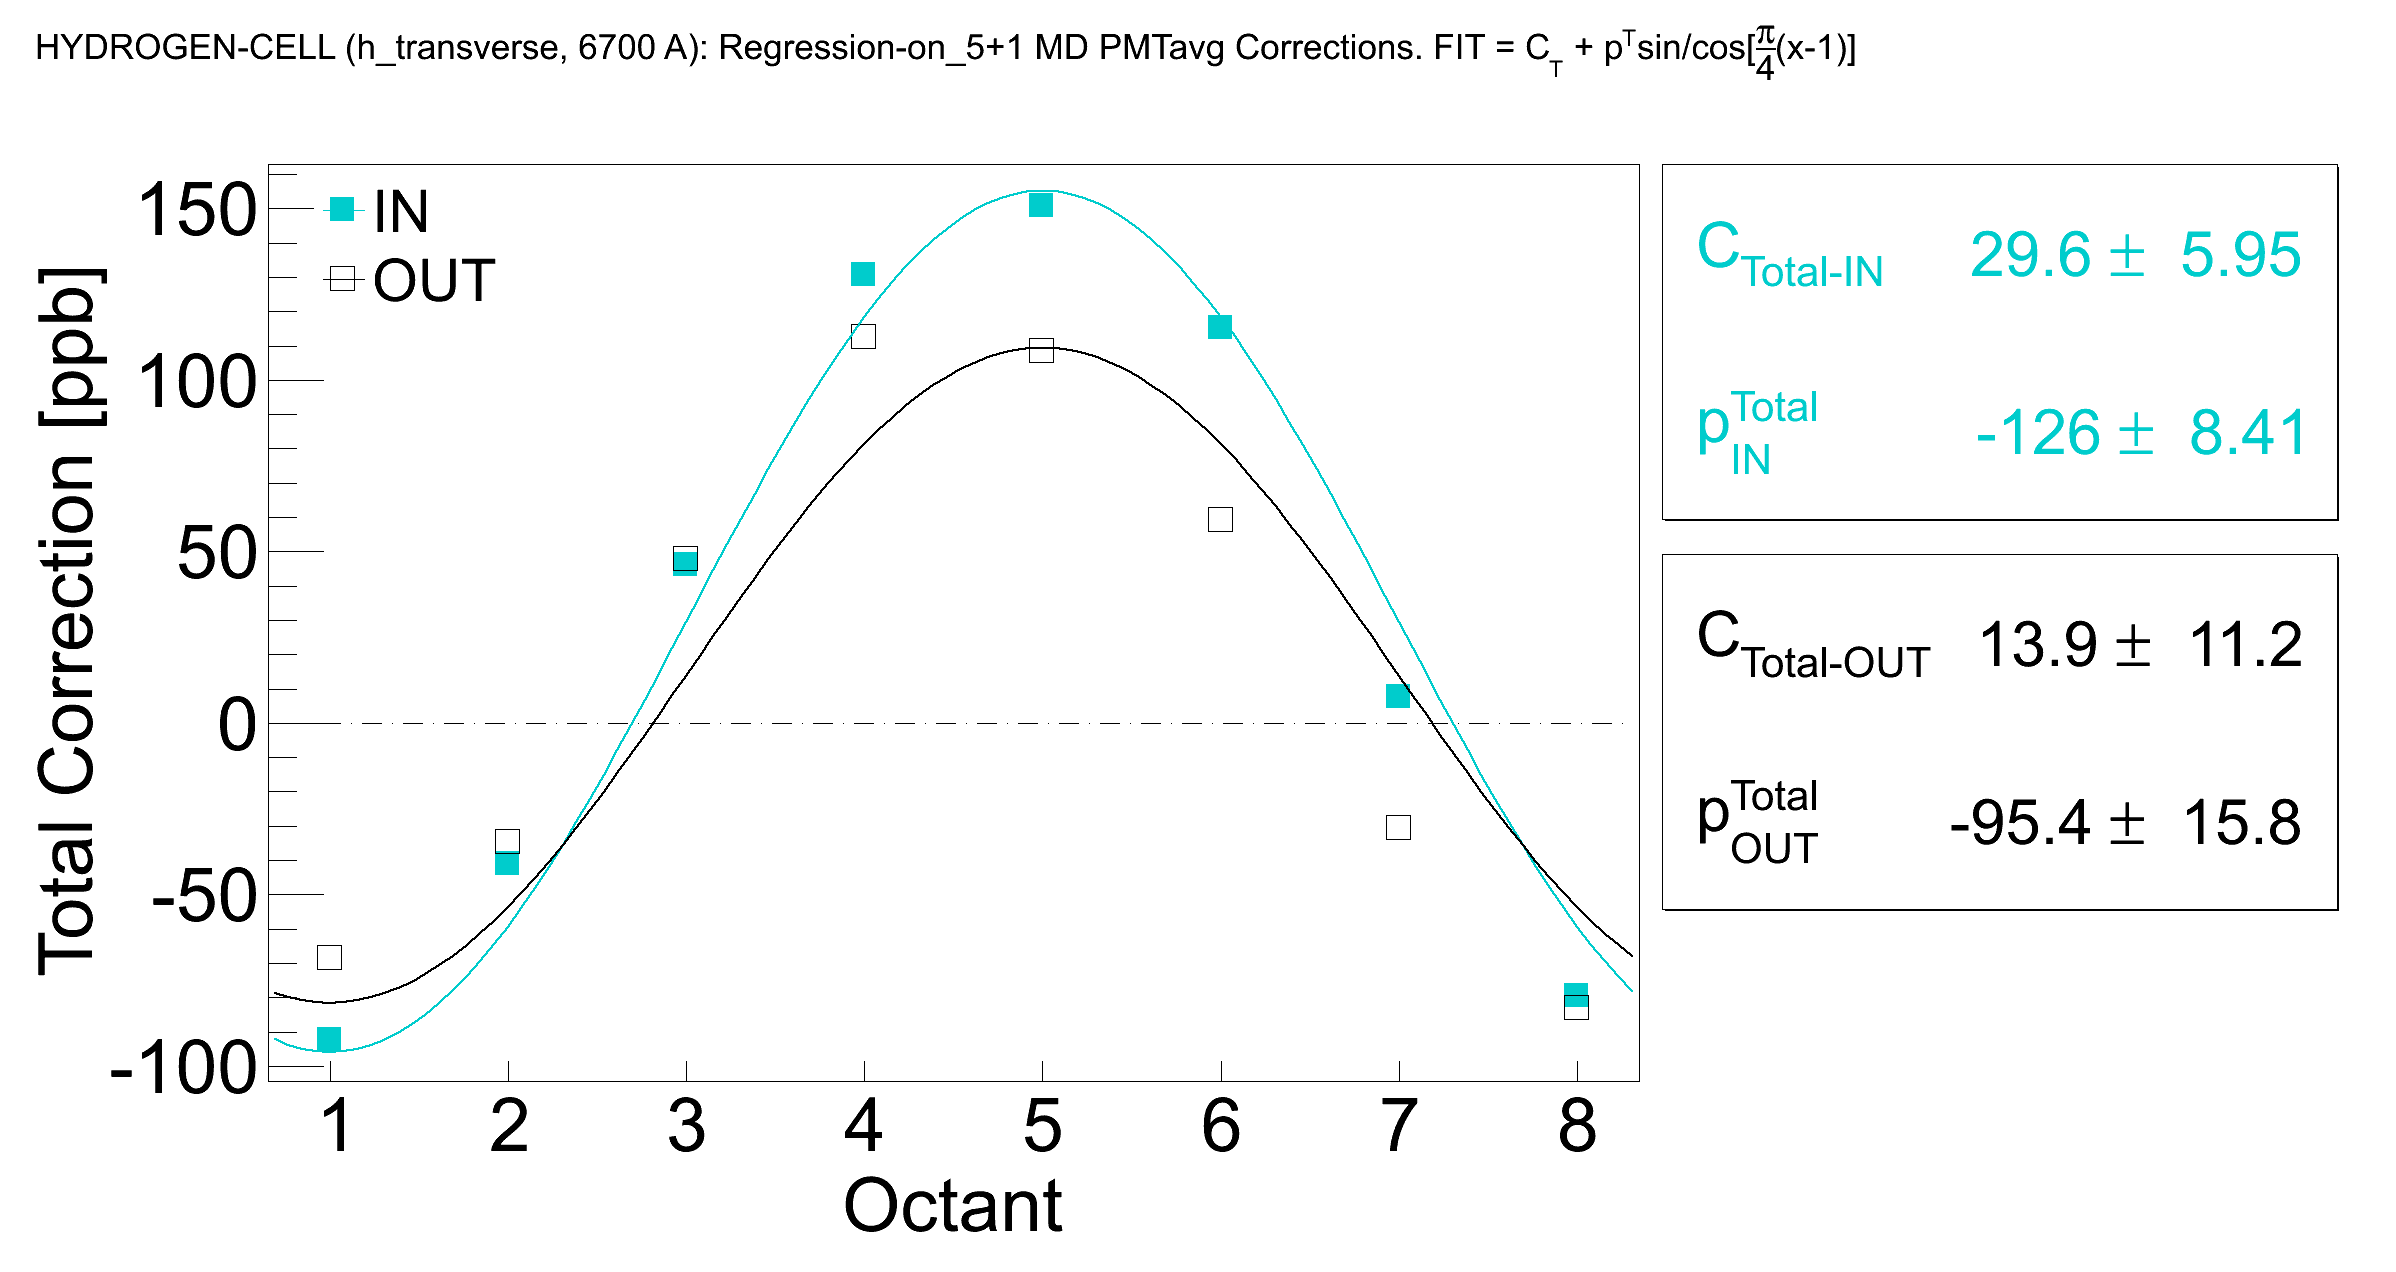
\includegraphics[width=10.0cm]{figures/MD_h_transverse_5+1_TotalCorrections}
	\end{center}
	\caption
%	[Total corrections vs octant for horizontal transverse data set.]	
	{Total corrections in ``5+1" regression scheme vs octant for horizontal LH$_{2}$ transverse data set are shown here. The total correction is the sum of all the corrections (with sign) shown in Figure~\ref{fig:MD_h_transverse_5+1_corrections}.}
	\label{fig:MD_h_transverse_5+1_TotalCorrections}
\end{figure}



%%\begin{figure}[!h]
%%	\begin{center}
%%	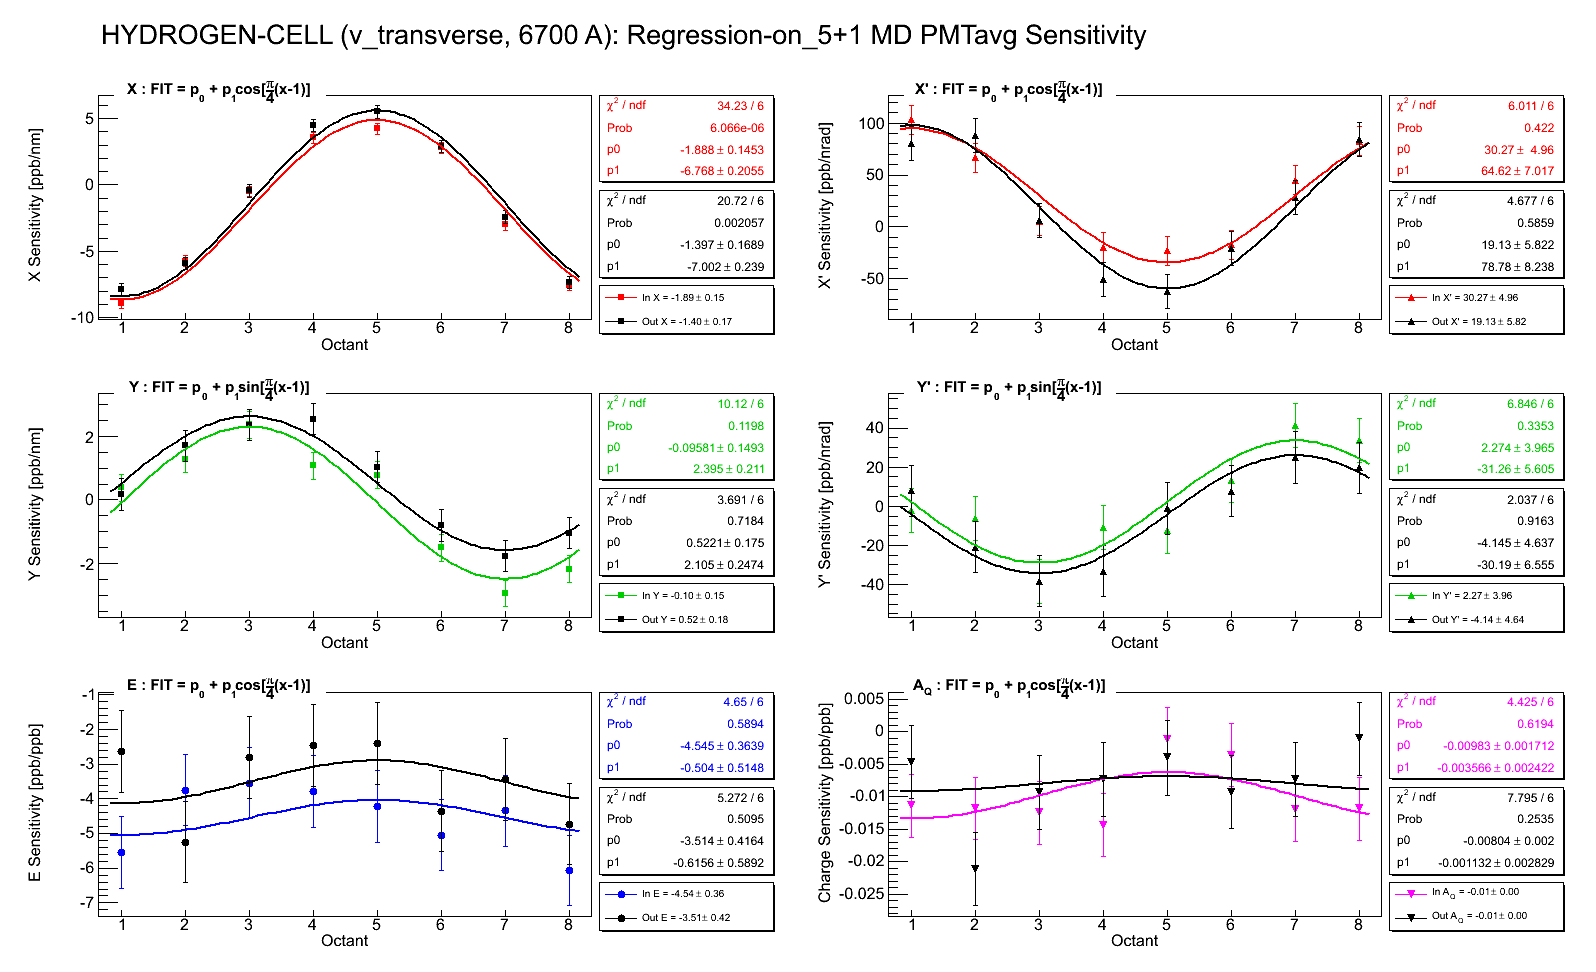
\includegraphics[width=15.0cm]{figures/transverse_LH2_v_transverse_5+1_sensitivity}
%%	\end{center}
%%	\caption{Main detector octant sensitivities with respect to 5+1 regression scheme for vertical transverse data set are shown here. Azimuthal dependence of the detector sensitivities to HCBA in the vertical LH$_{2}$ transverse data set. Beam positions and angles have sinusoidal dependence with octant. No such dependence is seen for energy and charge. Two IHWP states are shown separately for each beam parameter.}
%%	\label{fig:transverse_LH2_v_transverse_5+1_sensitivity}
%%\end{figure}
%
%\begin{figure}[!h]
%	\begin{center}
%	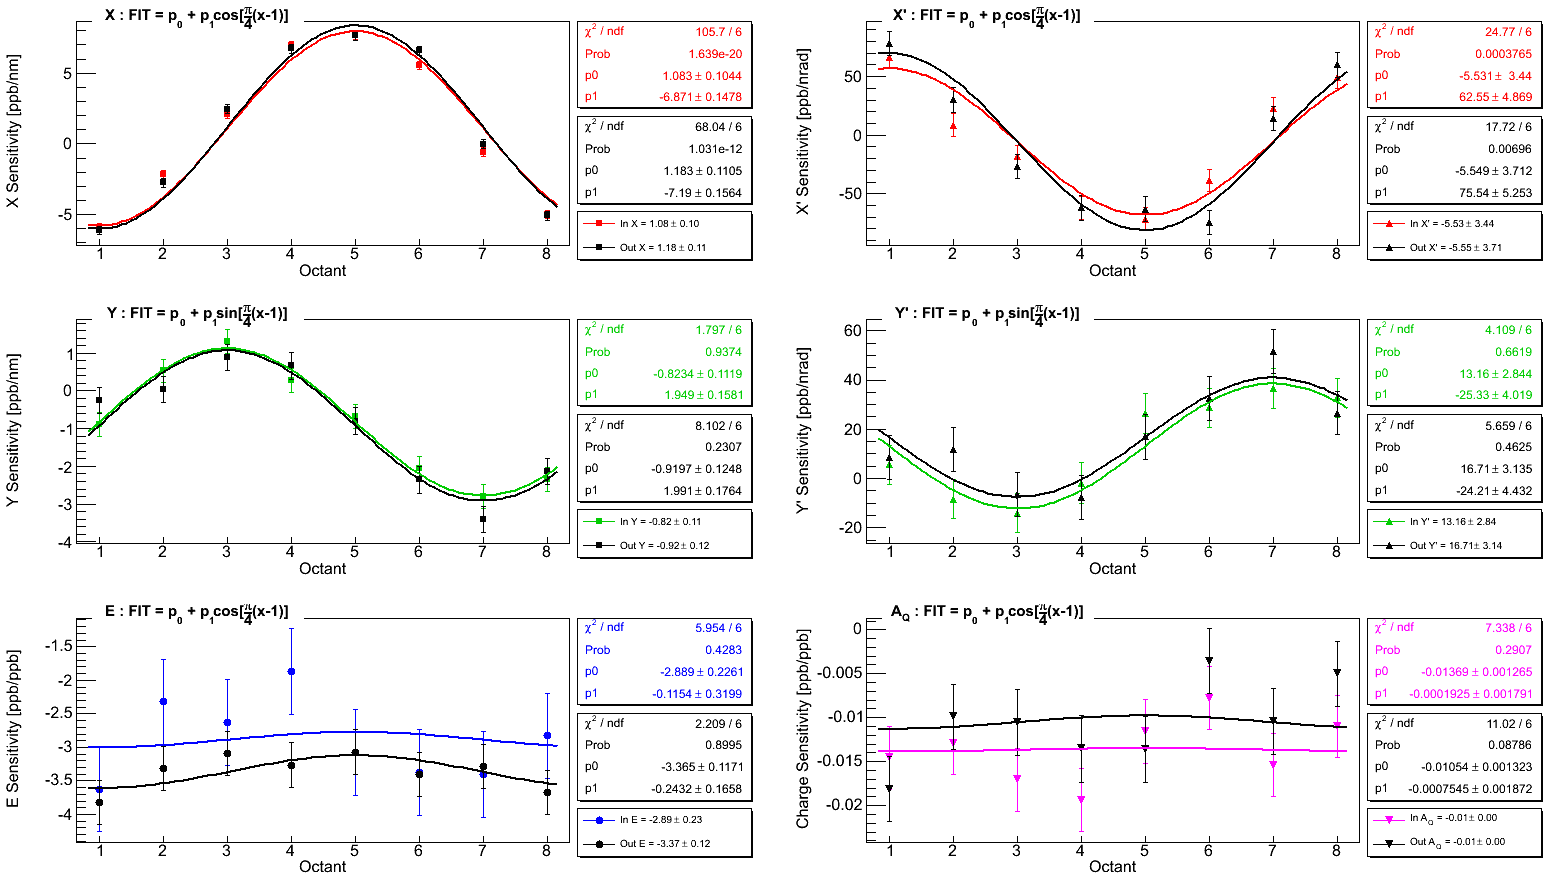
\includegraphics[width=15.0cm]{figures/transverse_LH2_h_transverse_5+1_sensitivity}
%	\end{center}
%	\caption
%	[Main detector sensitivities with respect to 5+1 regression scheme for horizontal transverse data set.]	
%	{Main detector octant sensitivities with respect to 5+1 regression scheme for horizontal transverse data set are shown here. Azimuthal dependence of the detector sensitivities to HCBA in the horizontal LH$_{2}$ transverse data set. Beam positions and angles have sinusoidal dependence with octant. No such dependence is seen for energy and charge. Two IHWP states are shown separately for each beam parameter. Fit functions used are also shown on the plot. The constant in the fit gives the error weighted average sensitivities. See APPENDIX-\ref{Beam Normal Single Spin Asymmetry in Inelastic e-p Scattering}, section~\ref{Corrections}  for the sensitivities and corrections from all data sets.}
%	\label{fig:transverse_LH2_h_transverse_5+1_sensitivity}
%\end{figure}
%
%
%\begin{figure}[!h]
%	\begin{center}
%	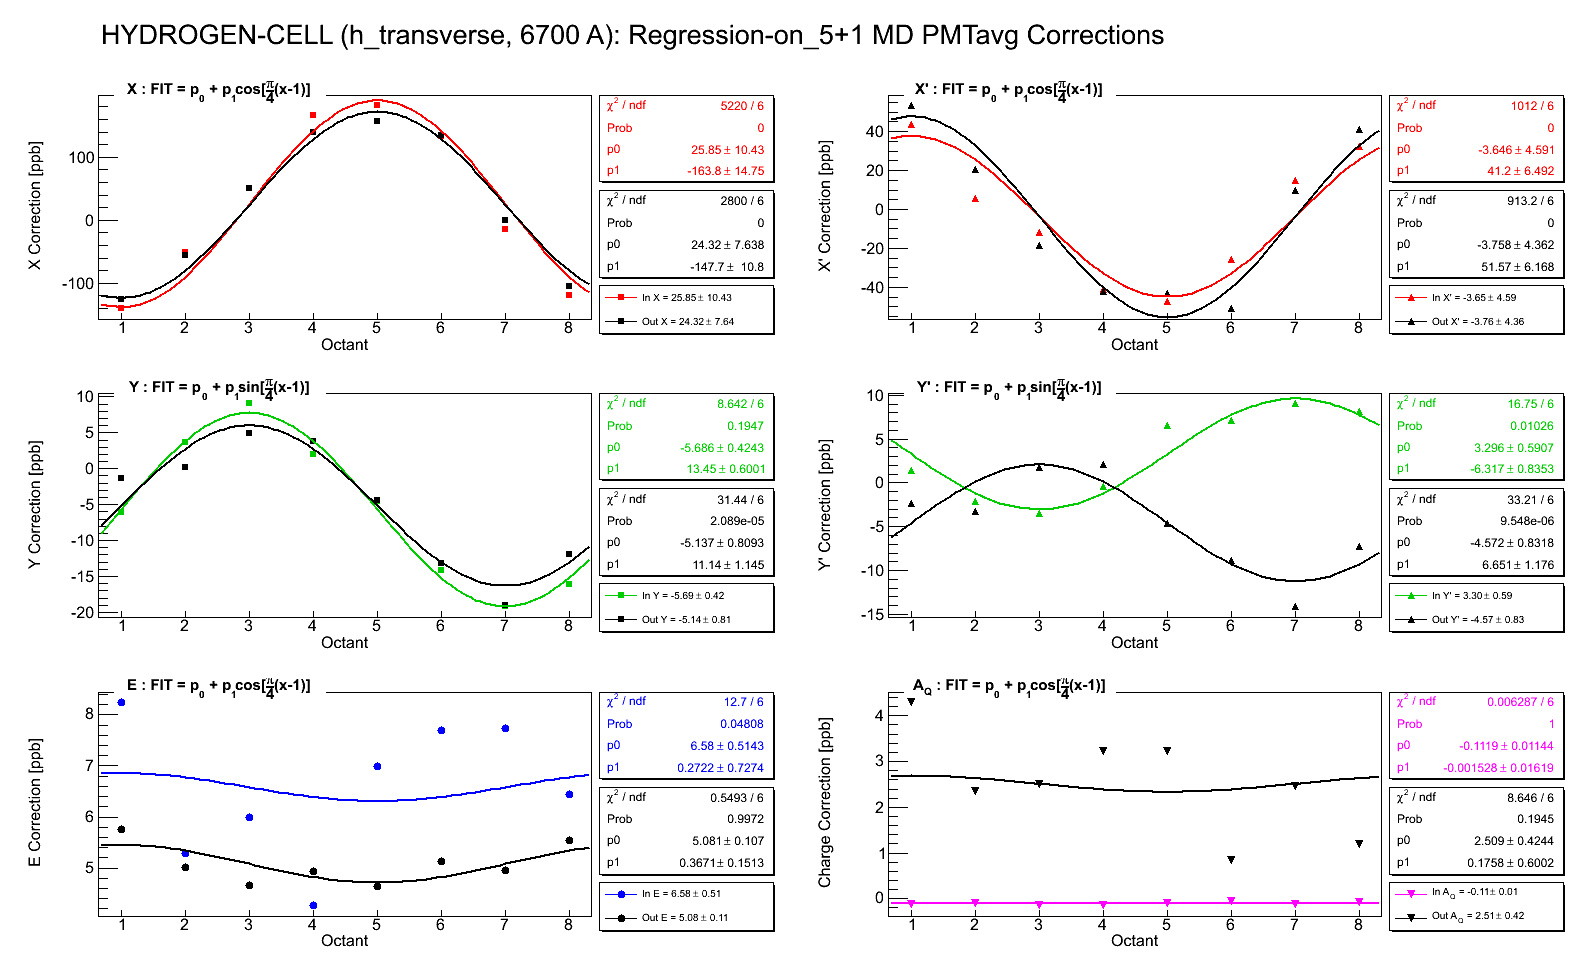
\includegraphics[width=15.0cm]{figures/transverse_LH2_h_transverse_5+1_correction}
%	\end{center}
%	\caption
%	[Main detector correction vs octant using to 5+1 regression scheme and differences for horizontal transverse data set.]	
%	{Main detector correction vs octant using to 5+1 regression scheme and differences for horizontal transverse data set are shown here. Azimuthal dependence of the corrections in the horizontal LH$_{2}$ transverse data set. Beam positions and angles have sinusoidal dependence with octant. No such dependence is seen for energy and charge. Two IHWP states are shown separately for each beam parameter.}
%	\label{fig:transverse_LH2_h_transverse_5+1_correction}
%\end{figure}
%
%
%%\begin{figure}[!h]
%%	\begin{center}
%%	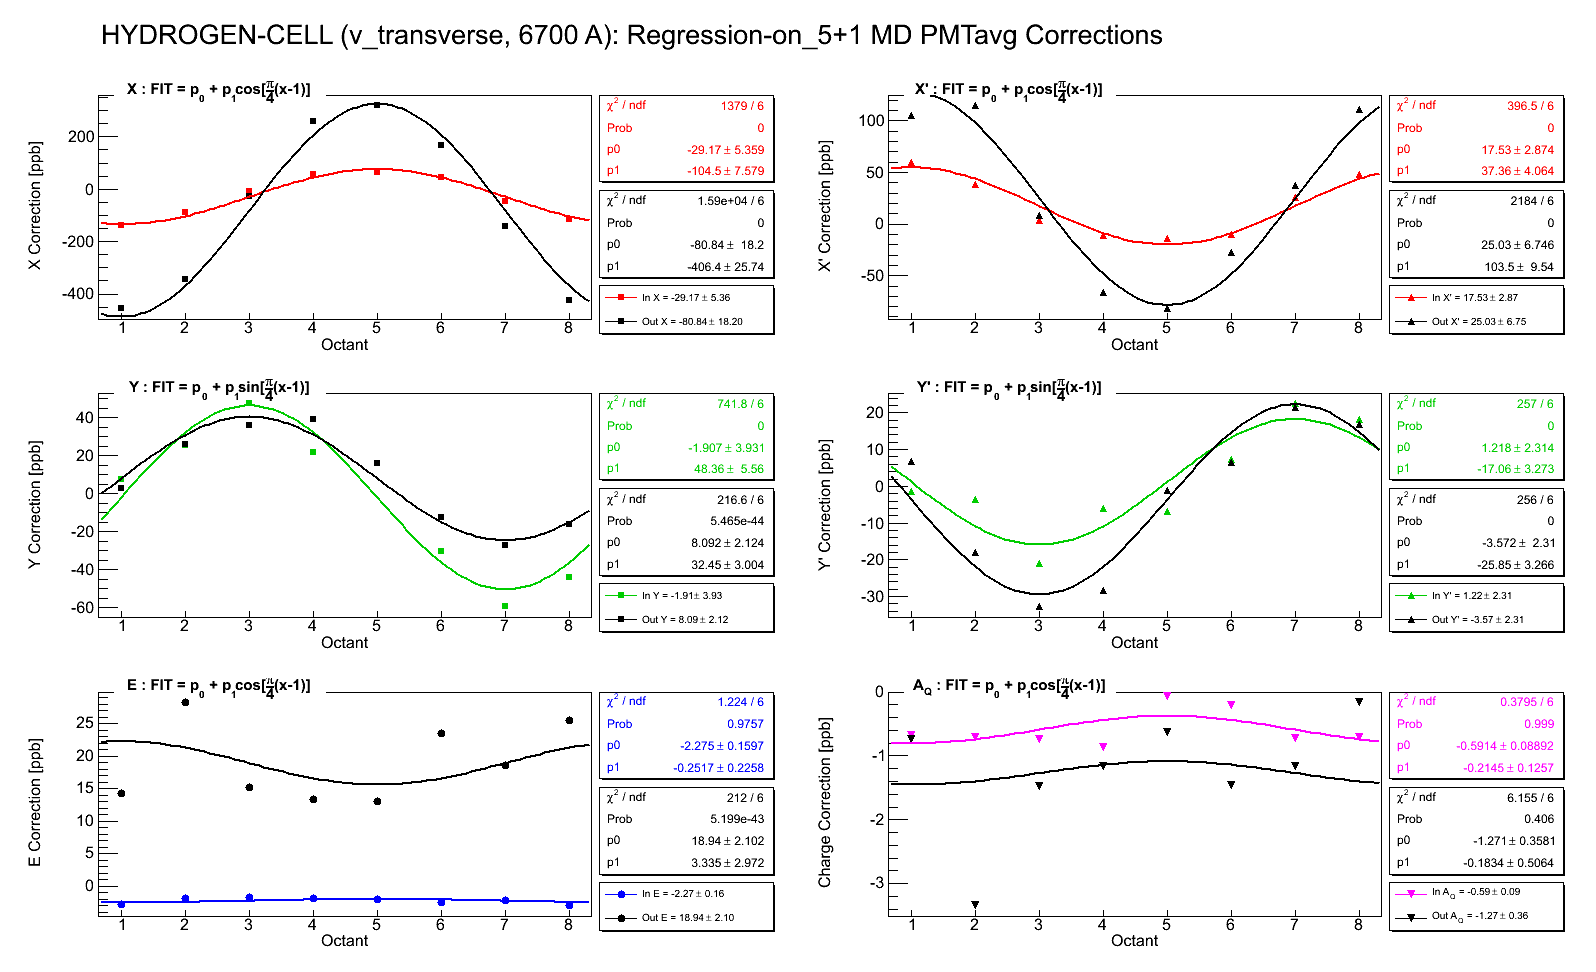
\includegraphics[width=15.0cm]{figures/transverse_LH2_v_transverse_5+1_correction}
%%	\end{center}
%%	\caption{Main detector correction vs octant using to 5+1 regression scheme and differences for vertical transverse data set are shown here. Azimuthal dependence of the corrections in the vertical LH$_{2}$ transverse data set. Beam positions and angles have sinusoidal dependence with octant. No such dependence is seen for energy and charge. Two IHWP states are shown separately for each beam parameter.}
%%	\label{fig:transverse_LH2_v_transverse_5+1_correction}
%%\end{figure}
%
%\begin{figure}[!h]
%	\begin{center}
%	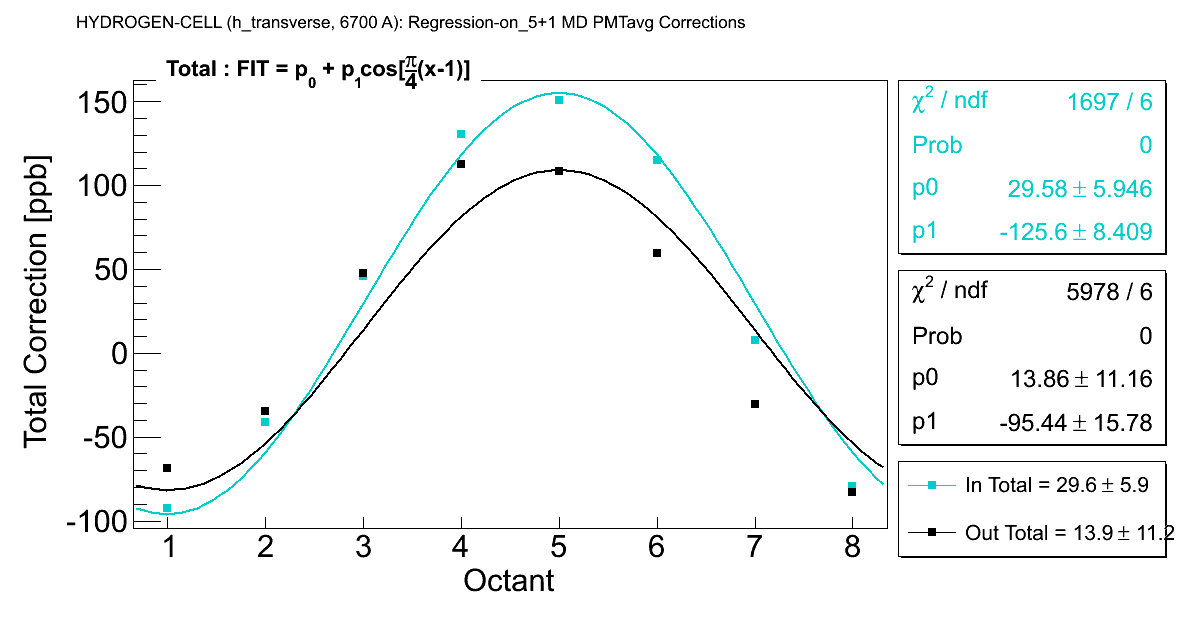
\includegraphics[width=15.0cm]{figures/transverse_LH2_h_transverse_5+1_total_correction}
%	\end{center}
%	\caption
%	[Total correction vs octant using to 5+1 regression scheme and differences for horizontal transverse data set.]
%	{Total correction vs octant using to 5+1 regression scheme and differences for horizontal transverse data set are shown here.}
%	\label{fig:transverse_LH2_h_transverse_5+1_total_correction}
%\end{figure}
%
%%\begin{figure}[!h]
%%	\begin{center}
%%	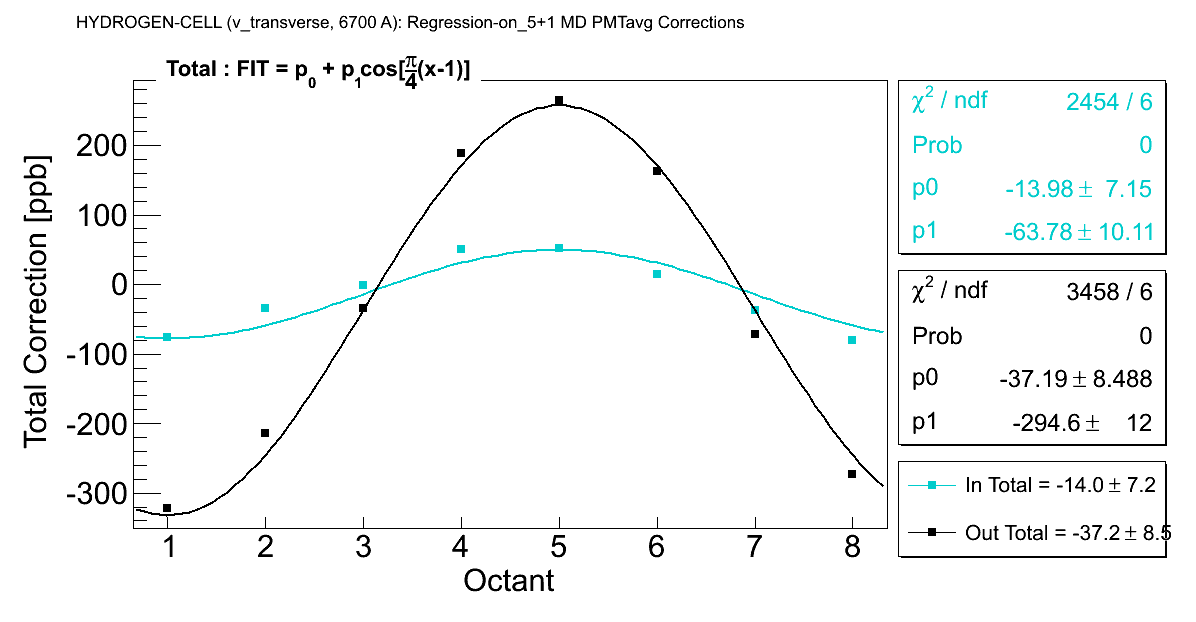
\includegraphics[width=15.0cm]{figures/transverse_LH2_v_transverse_5+1_total_correction}
%%	\end{center}
%%	\caption{Total correction vs octant using to 5+1 regression scheme and differences for vertical transverse data set are shown here.}
%%	\label{fig:transverse_LH2_v_transverse_5+1_total_correction}
%%\end{figure}

\begin{figure}[!h]
	\begin{center}
	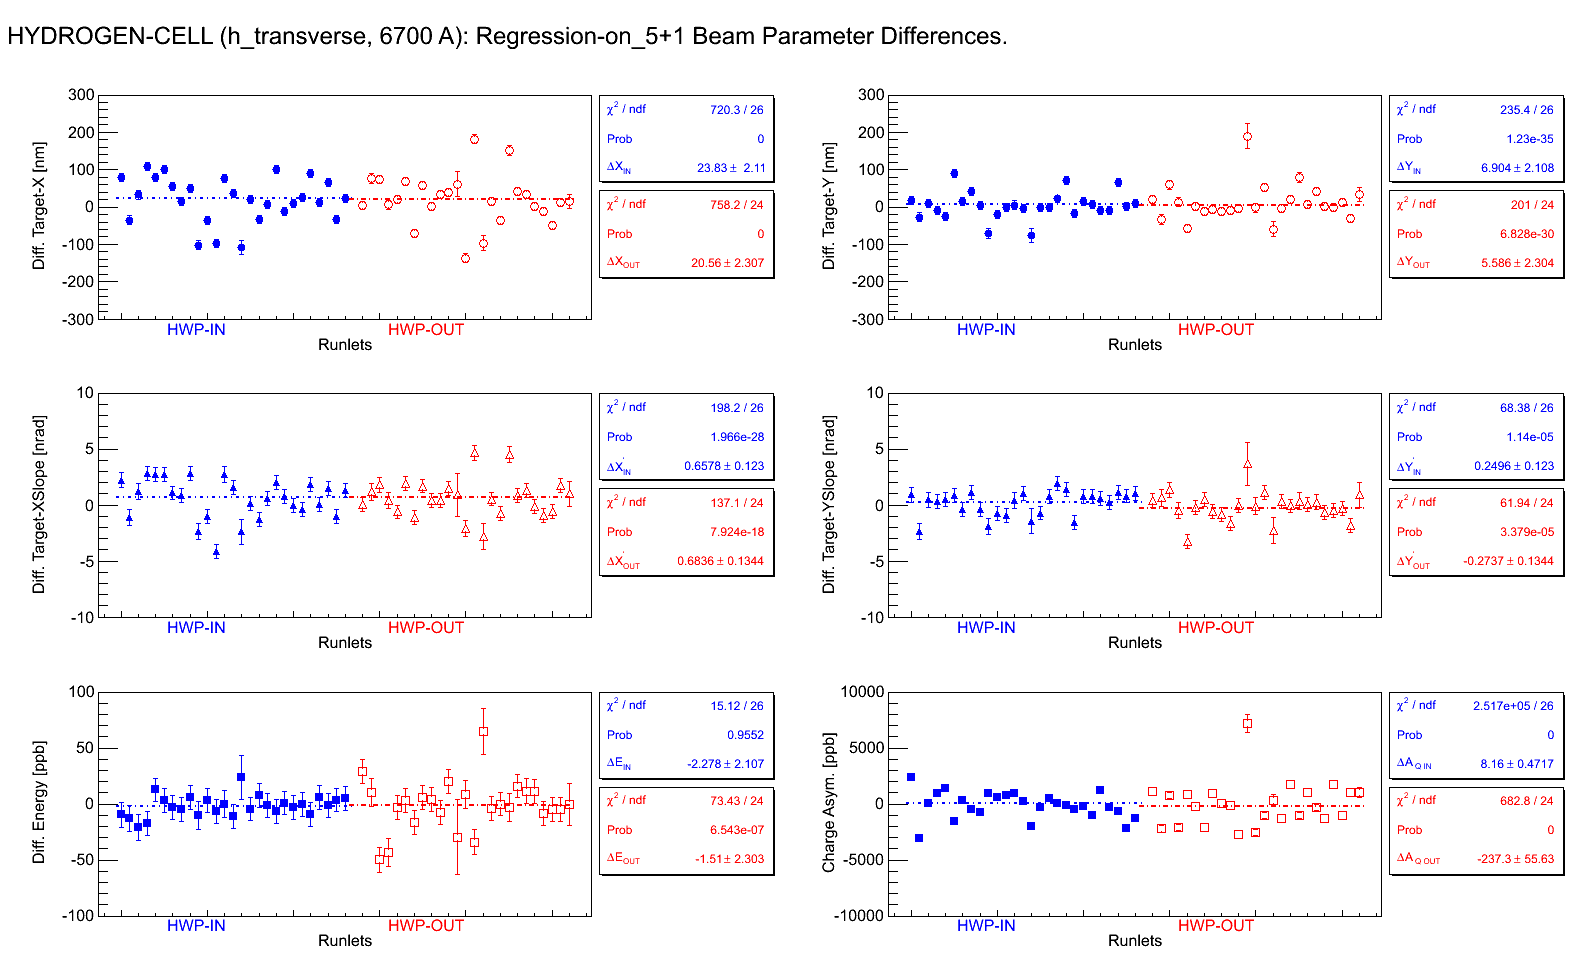
\includegraphics[width=15.0cm]{figures/transverse_LH2_h_diff}
	\end{center}
	\caption
%	[Beam position differences for horizontal transverse data set.]
	{Beam position differences for horizontal transverse data set.}
	\label{fig:transverse_LH2_h_diff}
\end{figure}

\begin{figure}[!h]
	\begin{center}
	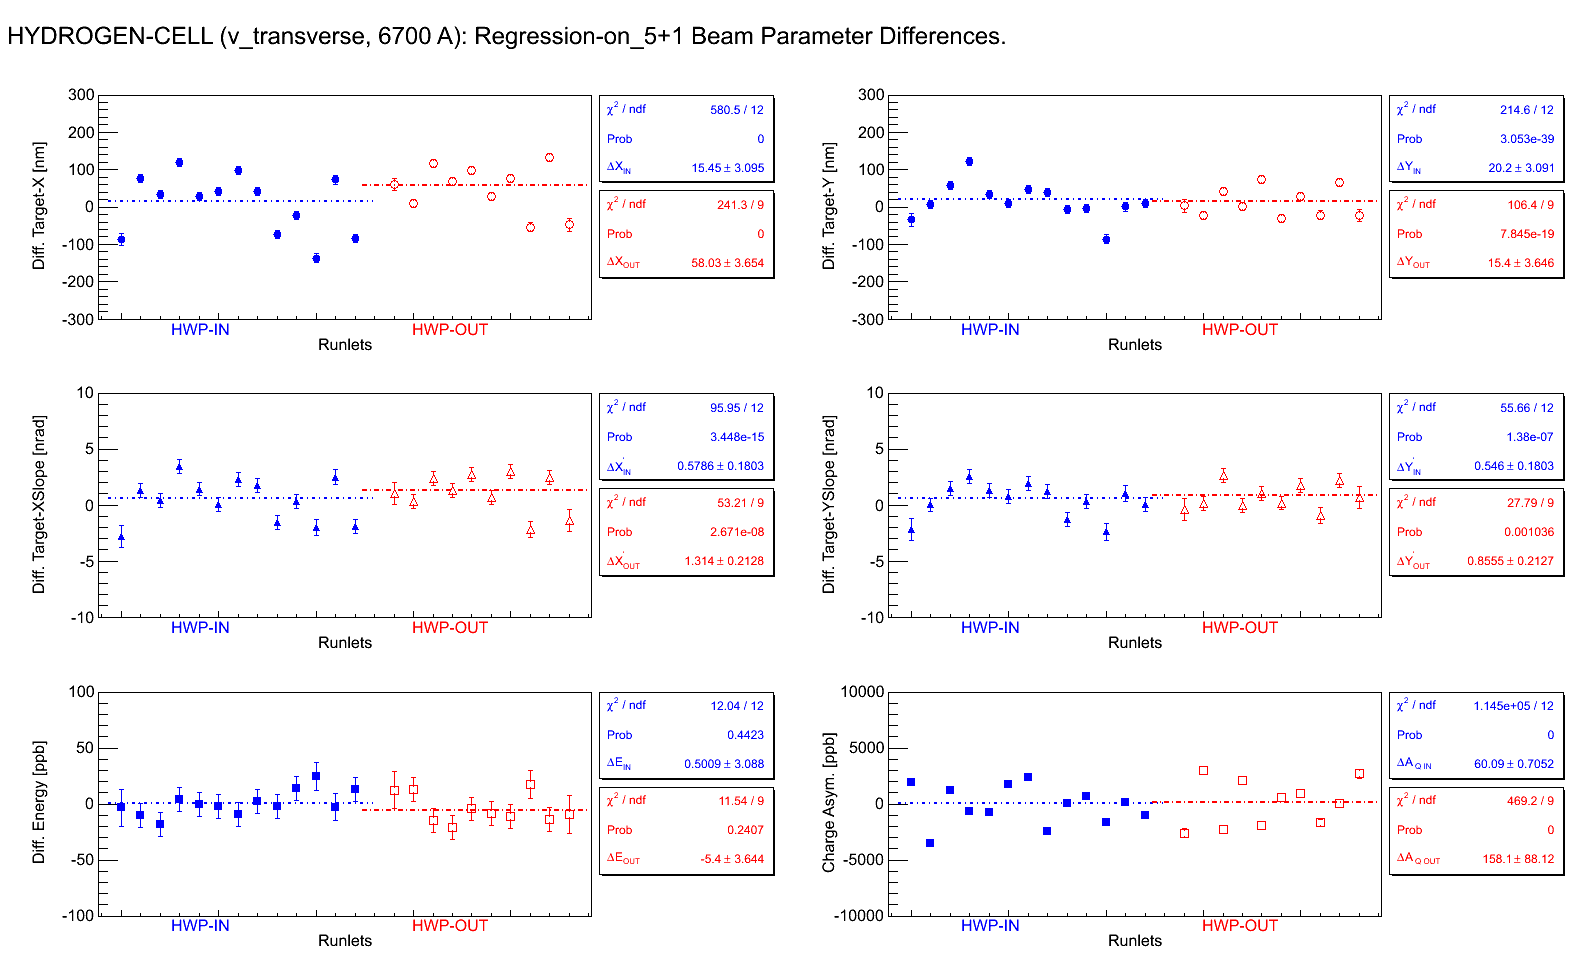
\includegraphics[width=15.0cm]{figures/transverse_LH2_v_diff}
	\end{center}
	\caption
%	[Beam position differences for vertical transverse data set.]
	{Beam position differences for vertical transverse data set.}
	\label{fig:transverse_LH2_v_diff}
\end{figure}

%%%%%%%%%%%%%%%%%%%%%%%%%%%%%%%%%%%%%%%%%%%%%%%%%%%%%%%%%%%%%
\section{Barsum vs PMTavg Asymmetries}
\label{Barsum vs PMTavg Asymmetries}
%%
Different ways to calculate the asymmetries. In case of barsum asymmetries we match gain of PMTs and then sum their yields and form asymmetries, whereas PMTavg asymmetries were formed as individual PMT asymmetries and then averaged. PMTavg and barsum asymmetries are shown in section~\ref{Asymmetry Correction using Linear Regression} and Figures~\ref{fig:BarsumAsym_on_5+1_h-LH2},~\ref{fig:BarsumAsym_on_5+1_v-LH2}, respectively. Barsum and PMTavg asymmetries match within $\sim$ 0.0005~ppm.

\begin{table}[h]
\begin{center}
  	\caption
%  	[Barsum and PMTavg asymmetries.]
  	{Barsum and PMTavg asymmetries.}
  \begin{tabular}{ c | c | c | c }
%    \hline
    \noalign{\hrule height 1pt}
    \multirow{2}{*}{Asymmetries} 	&	Barsum	&	PMTavg	&	Difference	\\
    			 		&	[ppm]		&	[ppm]	&	[ppm]	\\
%	\hline
    \noalign{\hrule height 1pt}
	$\epsilon_{reg}^{H}$ & 5.34291 &	5.34293 &	0.00002 \\
	$\epsilon_{reg}^{V}$ & 4.52568 &	4.52522 &	0.00046 \\
%    \hline
    \noalign{\hrule height 1pt}
  	\end{tabular}
  \label{tab:BarsumPMTavgAsymmetries}
\end{center}
\end{table}

%\begin{center}
%\framebox[\frameboxsize][c]{Barsum and PMTavg asymmetries match within $\sim$ 0.0005~ppm.}
%\end{center}

\begin{singlespace}
\begin{figure}[!h]
	\begin{center}
	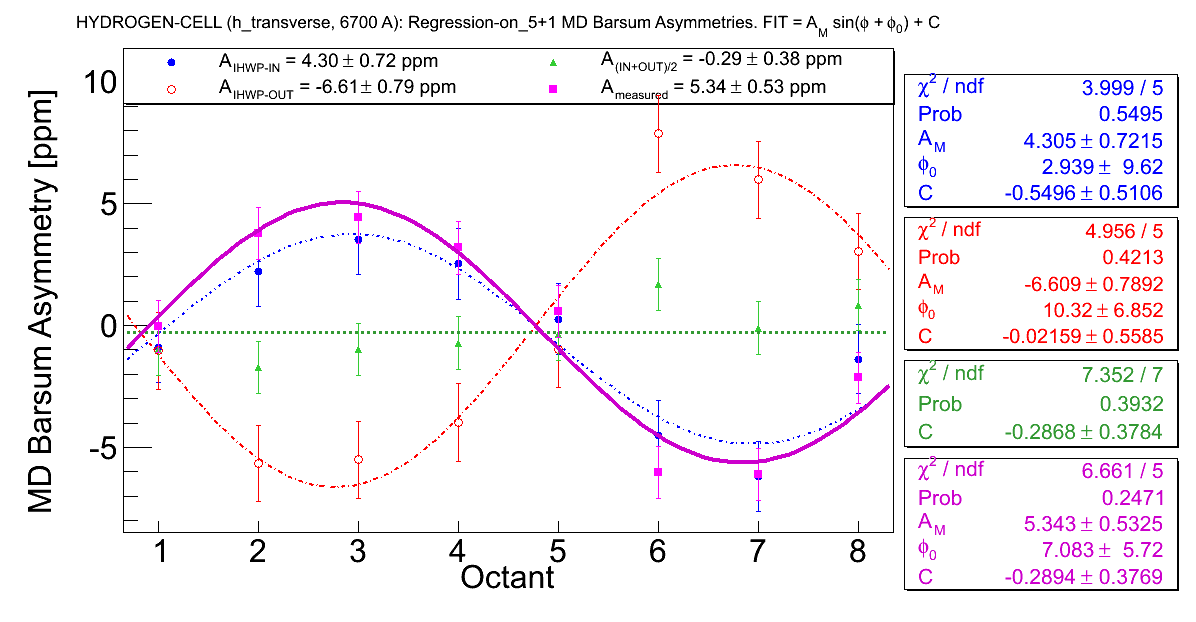
\includegraphics[width=15.0cm]{figures/BarsumAsym_on_5+1_h-LH2}
	\end{center}
	\caption
%	[Main detector barsum asymmetry for horizontal transverse at inelastic peak.]
	{Main detector barsum asymmetry for horizontal transverse at inelastic peak. For comparison, asymmetries for IN and OUT data are also shown separately. The regressed asymmetries change sign with the insertion of the IHWP with comparable amplitudes. }
	\label{fig:BarsumAsym_on_5+1_h-LH2}
\end{figure}
\end{singlespace}

\begin{singlespace}
\begin{figure}[!h]
	\begin{center}
	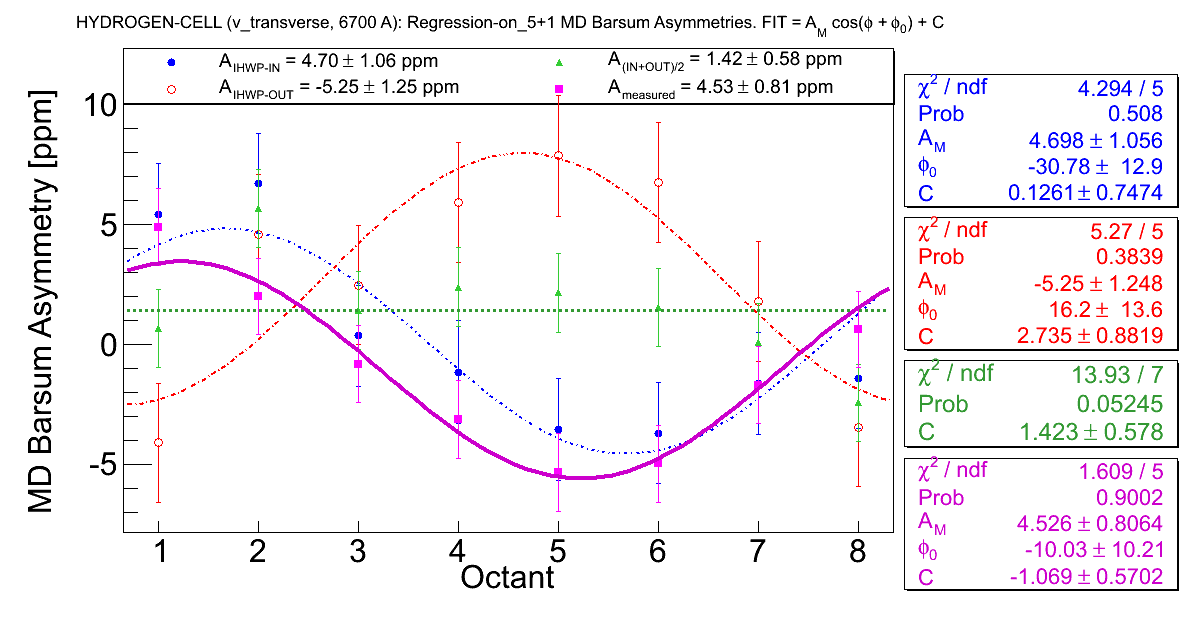
\includegraphics[width=15.0cm]{figures/BarsumAsym_on_5+1_v-LH2}
	\end{center}
	\caption
%	[Main detector barsum asymmetry for vertical transverse at inelastic peak.]
	{Main detector barsum asymmetry for vertical transverse at inelastic peak. For comparison, asymmetries for IN and OUT data are also shown separately. The regressed asymmetries change sign with the insertion of the IHWP with comparable amplitudes.}
	\label{fig:BarsumAsym_on_5+1_v-LH2}
\end{figure}
\end{singlespace}

%%%%%%%%%%%%%%%%%%%%%%%%%%%%%%%%%%%%%%%%%%%%%%%%%%%%%%%%%%%%%
\section{PMT Asymmetries}
\label{PMT Asymmetries}



\begin{singlespace}
\begin{figure}[!h]
	\begin{center}
	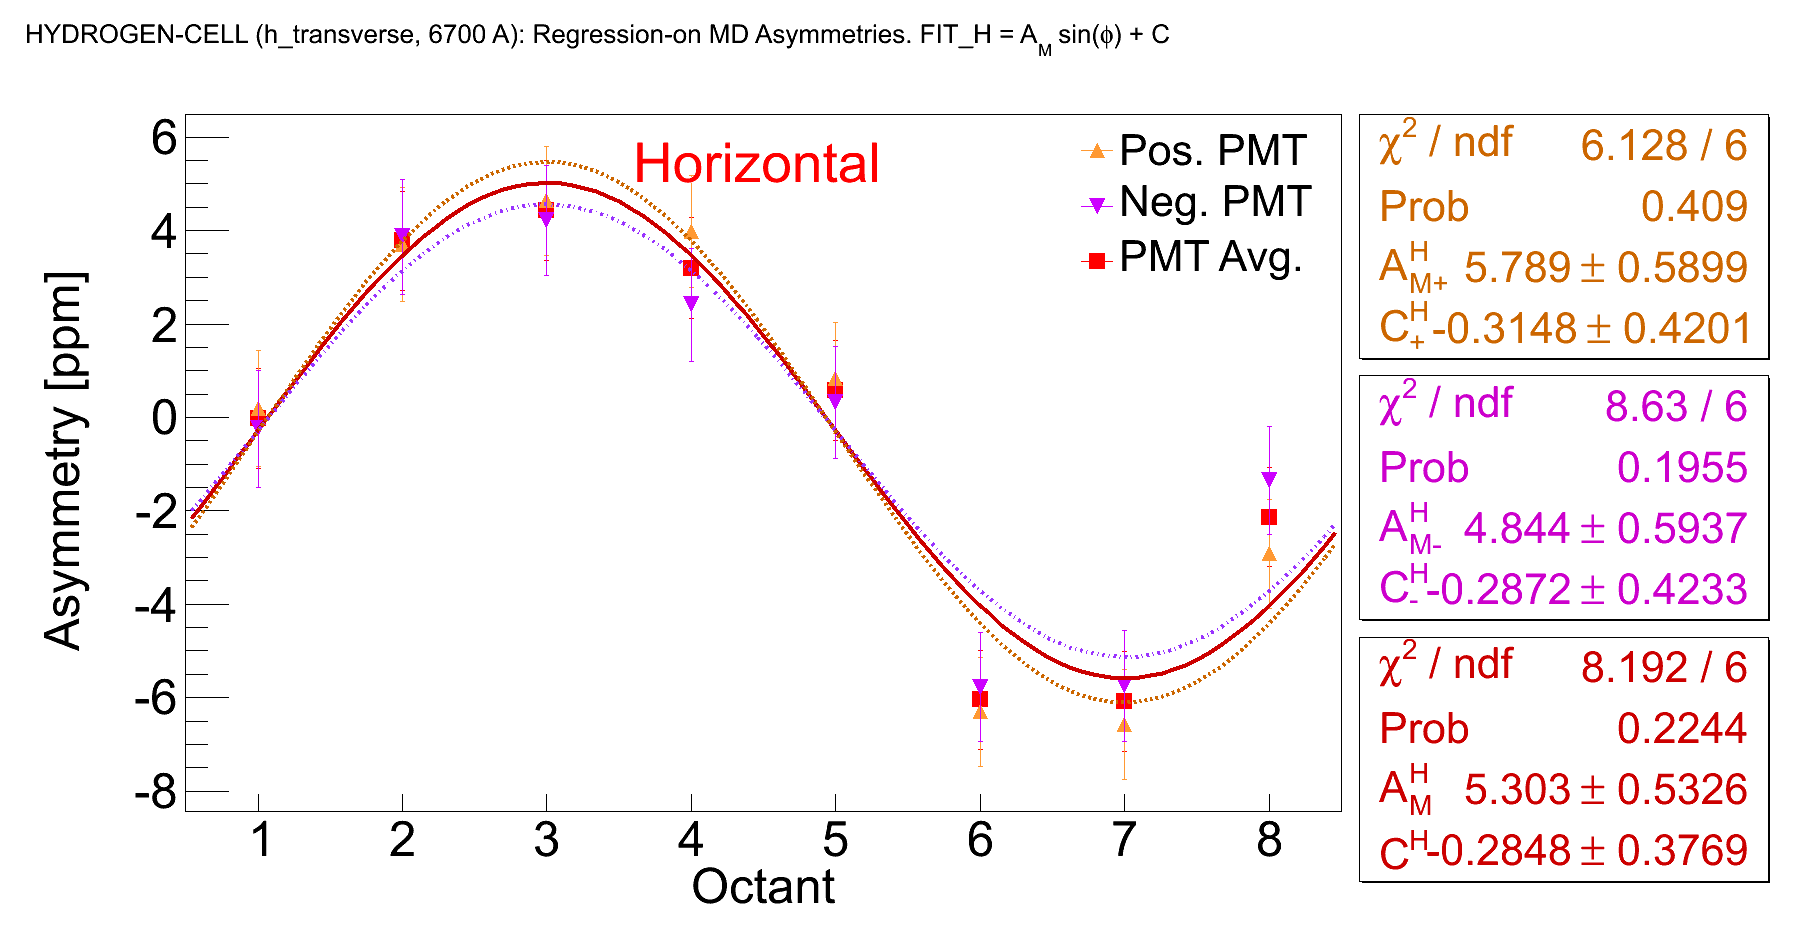
\includegraphics[width=15.0cm]{figures/MD_h_transverse_LH2_PMTAsymmetries_off_on}
	\end{center}
	\caption
%	[The POS, NEG PMTs and PMTavg asymmetries vs octant for inelastic horizontal transverse dataset.]
	{The individual fits over POS, NEG PMTs and PMTavg asymmetries vs octant for inelastic horizontal transverse dataset~\cite{elog:nur_ancillary145}.}
	\label{fig:MD_h_transverse_LH2_PMTAsymmetries_off_on}
\end{figure}
\end{singlespace}

\begin{singlespace}
\begin{figure}[!h]
	\begin{center}
	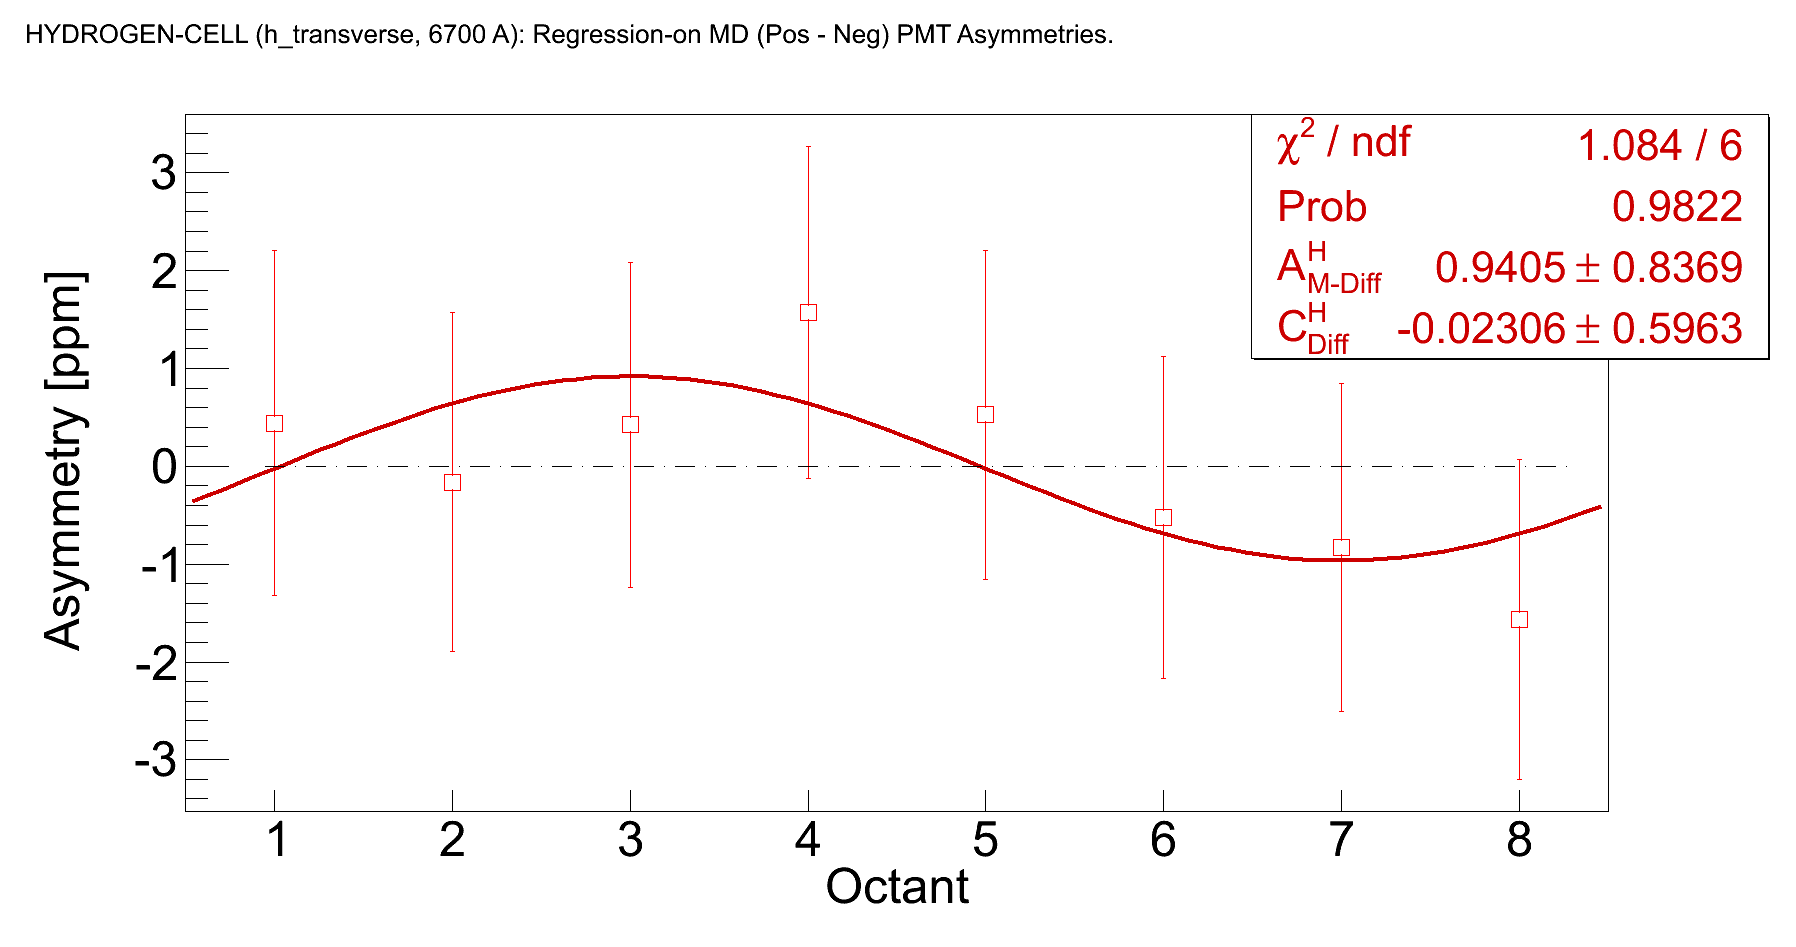
\includegraphics[width=15.0cm]{figures/MD_h_transverse_LH2_PMTAsymmetriesDiff_off_on}
	\end{center}
	\caption
%	[Difference between POS-NEG asymmetries vs octant for inelastic horizontal transverse dataset.]
	{Difference between POS-NEG asymmetries vs octant for inelastic horizontal transverse dataset. The error here is the quadrature sum of the POS and NEG asymmetry errors. See Table 1 for the values~\cite{elog:nur_ancillary145}.}
	\label{fig:MD_h_transverse_LH2_PMTAsymmetriesDiff_off_on}
\end{figure}
\end{singlespace}

\begin{singlespace}
\begin{figure}[!h]
	\begin{center}
	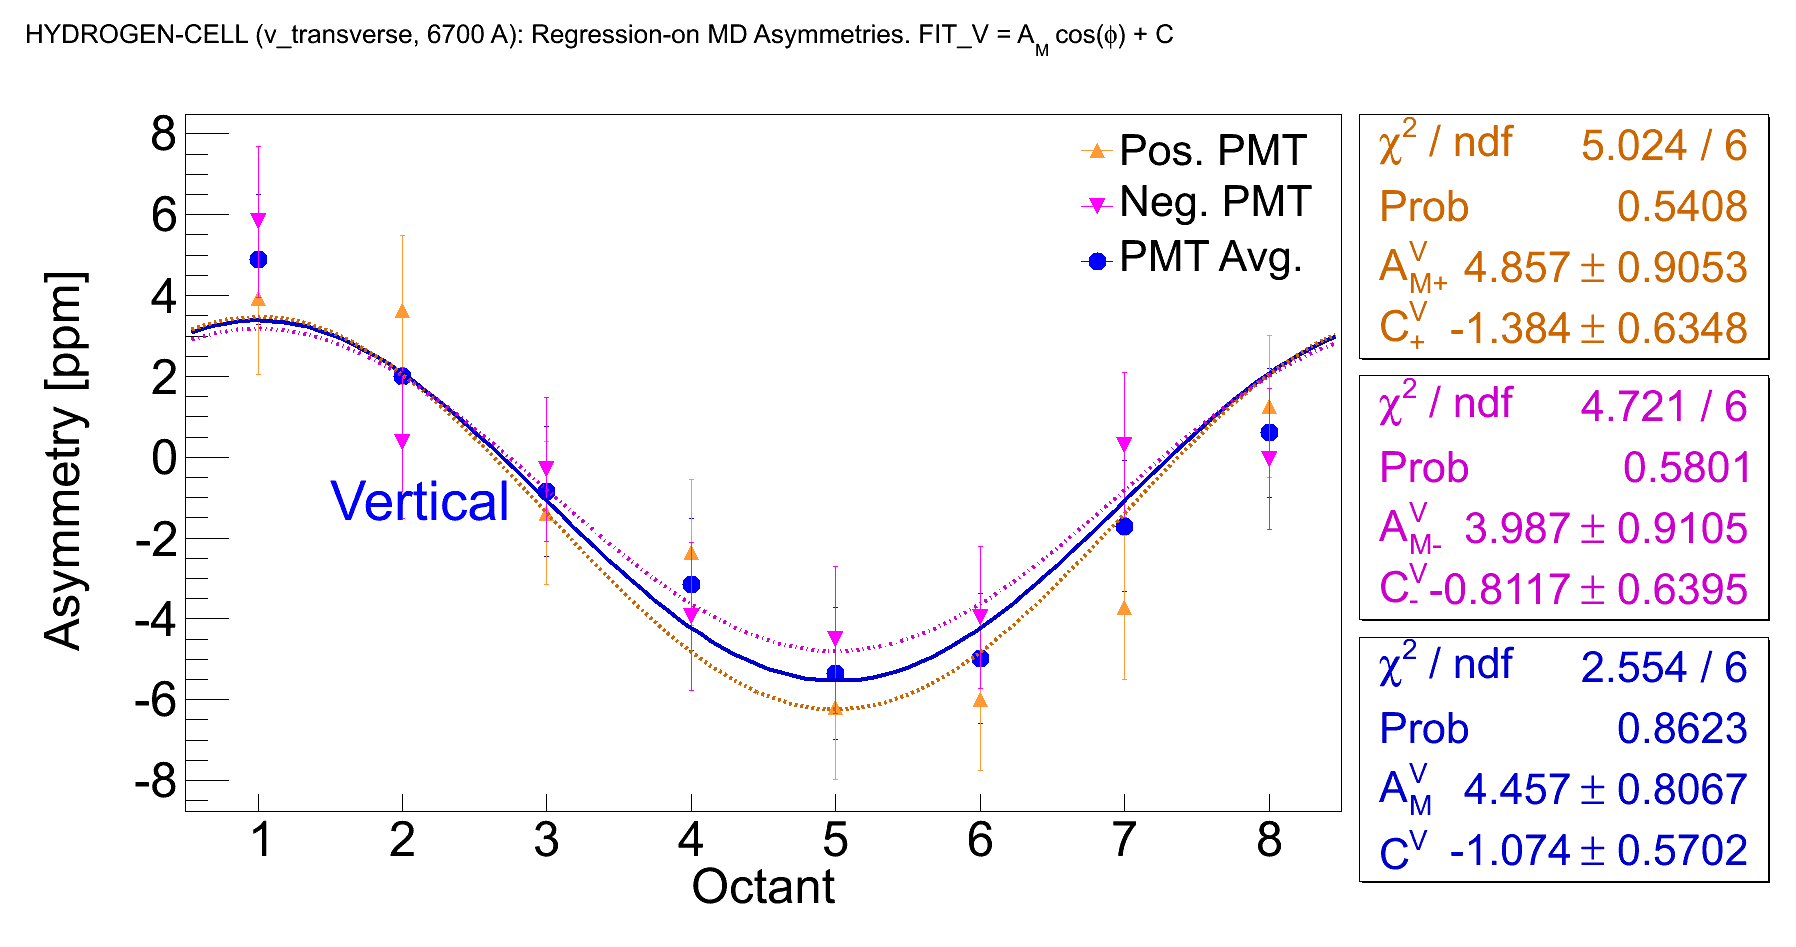
\includegraphics[width=15.0cm]{figures/MD_v_transverse_LH2_PMTAsymmetries_off_on}
	\end{center}
	\caption
%	[The POS, NEG PMTs and PMTavg asymmetries vs octant for inelastic vertical transverse dataset.]
	{The individual fits over POS, NEG PMTs and PMTavg asymmetries vs octant for inelastic vertical transverse dataset~\cite{elog:nur_ancillary145}.}
	\label{fig:MD_v_transverse_LH2_PMTAsymmetries_off_on}
\end{figure}
\end{singlespace}

\begin{singlespace}
\begin{figure}[!h]
	\begin{center}
	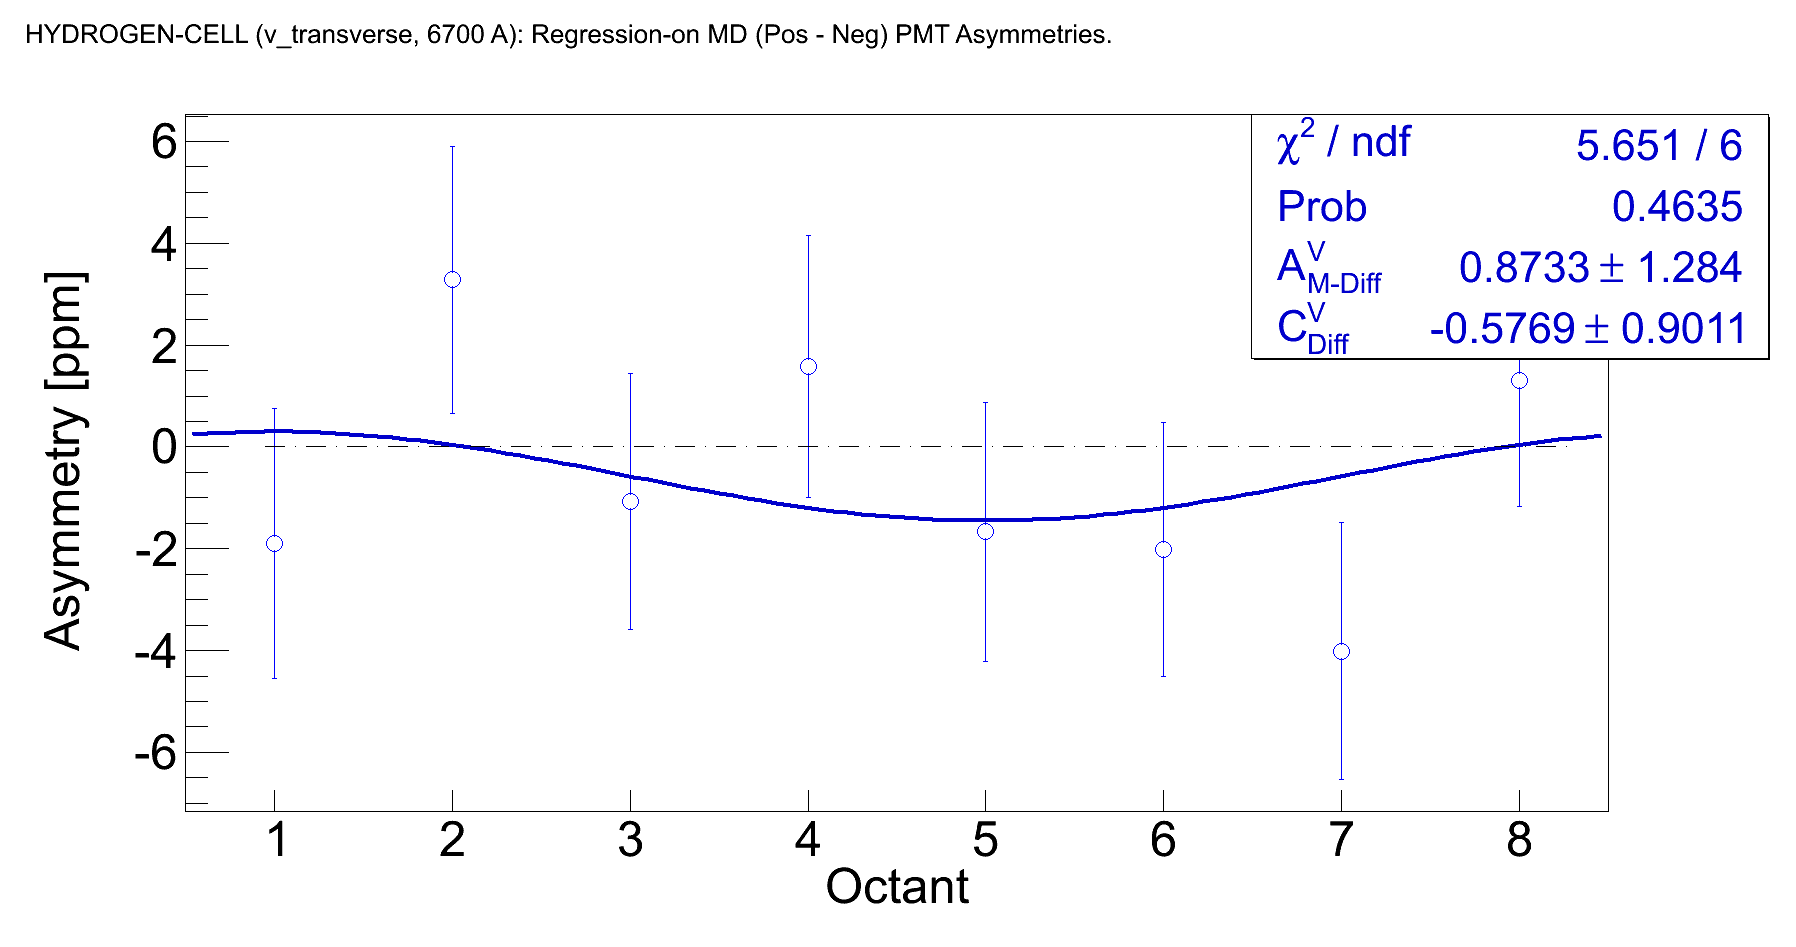
\includegraphics[width=15.0cm]{figures/MD_v_transverse_LH2_PMTAsymmetriesDiff_off_on}
	\end{center}
	\caption
%	[Difference between POS-NEG asymmetries vs octant for inelastic vertical transverse dataset.]
	{Difference between POS-NEG asymmetries vs octant for inelastic vertical transverse dataset. The error here is the quadrature sum of the POS and NEG asymmetry errors. See Table 1 for the values~\cite{elog:nur_ancillary145}.}
	\label{fig:MD_v_transverse_LH2_PMTAsymmetriesDiff_off_on}
\end{figure}
\end{singlespace}



%%%%%%%%%%%%%%%%%%%%%%%%%%%%%%%%%%%%%%%%%%%%%%%%%%%%%%%%%%%%%
\section{Detector Sensitivities}
\label{Detector Sensitivities}

%\begin{table}[!h]
%\begin{center}
%  \begin{tabular}{ c  c  c  c  c  c  c }
%    \hline
%    Detector	&	$\frac{\partial A}{\partial X}$	&	$\frac{\partial A}{\partial X^{\prime}}$	&	$\frac{\partial A}{\partial Y}$	&	$\frac{\partial A}{\partial Y^{\prime}}$	&	$\frac{\partial A}{\partial E}$	&	$\frac{\partial A}{\partial A_{Q}}$   \\
%	&	[ppb/nm]	&	[ppb/nrad]	&	[ppb/nm]	&	[ppb/nrad]	&	[ppb/ppb]	&	[ppb/ppb] \\
%	\hline
%	MD1 & -5.9079$\pm$0.294805 & -6.13277$\pm$0.311993 & & & & \\
%	MD2 & -2.16273$\pm$0.293545 & -2.73979$\pm$0.310751 & & & & \\
%	MD3 & 2.10449$\pm$0.29483 & 2.44739$\pm$0.312561 & & & & \\
%	MD4 & 6.97749$\pm$0.298471 & 6.74414$\pm$0.315152 & & & & \\
%	MD5 & 7.66108$\pm$0.297984 & 7.65709$\pm$0.315616 & & & & \\
%	MD6 & 5.56704$\pm$0.294654 & 6.58009$\pm$0.311996 & & & & \\
%	MD7 & -0.584922$\pm$0.296162 & -0.0127185$\pm$0.313588 & & & & \\
%	MD8 & -4.97869$\pm$0.292054 & -5.08178$\pm$0.309367 & & & & \\
%    \hline
%  	\end{tabular}
%  	\caption[Sensitivities.]{Sensitivities.}
%  \label{sensitivities}
%\end{center}
%\end{table}


\begin{table}[!h]
\begin{center}
  	\caption
%  	[MD Sensitivities for X and Y.]
  	{MD Sensitivities for X and Y.}
    \begin{tabular}{c|cc|cc}
%    \hline
    \noalign{\hrule height 1pt}
%      \multicolumn{1}{c}{} & & & & & & \\[\dimexpr-\normalbaselineskip-\arrayrulewidth]% Correct for mis-alignment
    \multirow{3}{*}{Detector}	&	\multicolumn{2}{ c}{$\frac{\partial \epsilon}{\partial X}$} & \multicolumn{2}{|c}{$\frac{\partial \epsilon}{\partial Y}$}  \\
	&	\multicolumn{2}{ c}{[ppb/nm]}	&	\multicolumn{2}{|c}{[ppb/nm]} \\ 
%	\hline
	\cline{2-5}
	& HWP-IN & HWP-OUT & HWP-IN & HWP-OUT \\
%	\hline
    \noalign{\hrule height 1pt}
	MD1 & -5.91$\pm$0.29 & -6.13$\pm$0.31 & -0.88$\pm$0.29	& -0.25$\pm$0.35 \\
	MD2 & -2.16$\pm$0.29 & -2.74$\pm$0.31 & 0.53$\pm$0.29 	& 0.04$\pm$0.35 \\
	MD3 & 2.10$\pm$0.29 & 2.44$\pm$0.31 & 1.32$\pm$0.29		& 0.89$\pm$0.35 \\
	MD4 & 6.98$\pm$0.30 & 6.74$\pm$0.32 & 0.29$\pm$0.30	& 0.67$\pm$0.36 \\
	MD5 & 7.66$\pm$0.30 & 7.66$\pm$0.32 & -0.67$\pm$0.30	& -0.80$\pm$0.36 \\
	MD6 & 5.57$\pm$0.29 & 6.58$\pm$0.31 & -2.05$\pm$0.30	& -2.35$\pm$0.35 \\
	MD7 & -0.58$\pm$0.30 & -0.01$\pm$0.31 & -2.79$\pm$0.30	& -3.41$\pm$0.35 \\
	MD8 & -4.98$\pm$0.29 & -5.08$\pm$0.31 & -2.34$\pm$0.29	& -2.14$\pm$0.35 \\
%    \hline
    \noalign{\hrule height 1pt}
    \end{tabular}
  \label{tab:sensitivities_hxy}
\end{center}
\end{table}




\begin{table}[!h]
\begin{center}
  	\caption
%  	[MD Sensitivities for X$^{\prime}$ and Y$^{\prime}$.]
  	{MD Sensitivities for X$^{\prime}$ and Y$^{\prime}$.}
    \begin{tabular}{c|cc|cc}
%    \hline
    \noalign{\hrule height 1pt}
    \multirow{3}{*}{Detector}	&	\multicolumn{2}{ c}{$\frac{\partial \epsilon}{\partial X^{\prime}}$} & \multicolumn{2}{|c}{$\frac{\partial \epsilon}{\partial Y^{\prime}}$}  \\
	&	\multicolumn{2}{ c}{[ppb/nrad]}	&	\multicolumn{2}{|c}{[ppb/nrad]} \\ 
%	\hline
	\cline{2-5}
	& HWP-IN & HWP-OUT & HWP-IN & HWP-OUT \\
%	\hline
    \noalign{\hrule height 1pt}
	MD1 & 66.31$\pm$9.71 & 78.33$\pm$10.48 & 5.54$\pm$8.03 & 8.56$\pm$8.85 \\
	MD2 & 8.61$\pm$9.67 & 30.13$\pm$10.44 & -8.33$\pm$8.00 & 11.81$\pm$8.82 \\
	MD3 & -18.33$\pm$9.71 & -26.87$\pm$10.50 & -14.08$\pm$8.032 & -6.59$\pm$8.87 \\
	MD4 & -62.14$\pm$9.83 & -61.88$\pm$10.58 & -1.82$\pm$8.13 & -7.78$\pm$8.94 \\
	MD5 & -71.83$\pm$9.82 & -63.13$\pm$10.60 & 26.31$\pm$8.12 & 16.87$\pm$8.95 \\
	MD6 & -38.80$\pm$9.71 & -74.72$\pm$10.48 & 28.69$\pm$8.03 & 32.50$\pm$8.85 \\
	MD7 & 22.40$\pm$9.76 & 14.19$\pm$10.53 & 36.49$\pm$8.068 & 51.75$\pm$8.90 \\
	MD8 & 49.43$\pm$9.62 & 59.98$\pm$10.39 & 32.82$\pm$7.96 & 26.52$\pm$8.78 \\
%    \hline
    \noalign{\hrule height 1pt}
    \end{tabular}
  \label{tab:sensitivities_hxpyp}
\end{center}
\end{table}


\begin{table}[!h]
\begin{center}
  	\caption
%  	[MD Sensitivities for E and A$_{Q}$.]
  	{MD Sensitivities for E and A$_{Q}$.}
    \begin{tabular}{c|cc|cc}
%    \hline
    \noalign{\hrule height 1pt}
%      \multicolumn{1}{c}{} & & & & & & \\[\dimexpr-\normalbaselineskip-\arrayrulewidth]% Correct for mis-alignment
    \multirow{3}{*}{Detector}	&	\multicolumn{2}{ c}{$\frac{\partial \epsilon}{\partial E}$} & \multicolumn{2}{|c}{$\frac{\partial \epsilon}{\partial A_{Q}}$}  \\
	&	\multicolumn{2}{ c}{[ppb/ppb]}	&	\multicolumn{2}{|c}{[ppb/ppb]} \\ 
%	\hline  
	\cline{2-5}
	& HWP-IN & HWP-OUT & HWP-IN & HWP-OUT \\
%	\hline
    \noalign{\hrule height 1pt}
	MD1 & -3.62$\pm$0.64 & -3.82$\pm$0.33 & -0.0146$\pm$0.0036 & -0.0181$\pm$0.0037 \\
	MD2 & -2.32$\pm$0.64 & -3.32$\pm$0.33 & -0.0129$\pm$0.0036 & -0.0099$\pm$0.0037 \\
	MD3 & -2.63$\pm$0.64 & -3.09$\pm$0.33 & -0.0171$\pm$0.0036 & -0.0105$\pm$0.0037 \\
	MD4 & -1.87$\pm$0.65 & -3.27$\pm$0.33 & -0.0194$\pm$0.0036 & -0.0135$\pm$0.0038 \\
	MD5 & -3.07$\pm$0.65 & -3.07$\pm$0.33 & -0.0116$\pm$0.0036 & -0.0136$\pm$0.0038 \\
	MD6 & -3.38$\pm$0.64 & -3.40$\pm$0.33 & -0.0078$\pm$0.0036 & -0.0036$\pm$0.0037 \\
	MD7 & -3.40$\pm$0.64 & -3.28$\pm$0.33 & -0.0154$\pm$0.0036 & -0.0104$\pm$0.0038 \\
	MD8 & -2.83$\pm$0.63 & -3.67$\pm$0.33 & -0.0110$\pm$0.0035 & -0.0050$\pm$0.0037 \\
%    \hline
    \noalign{\hrule height 1pt}
    \end{tabular}
  \label{tab:sensitivities_heq}
\end{center}
\end{table}





%\begin{landscape}
%
%\begin{table}[!h]
%\begin{center}
%    \begin{tabular}{c|cc|cc|cc|cc|cc|cc}
%      \hline
%%      \multicolumn{1}{c}{} & & & & & & \\[\dimexpr-\normalbaselineskip-\arrayrulewidth]% Correct for mis-alignment
%    Detector & \multicolumn{2}{|c}{$\frac{\partial A}{\partial X}$} & \multicolumn{2}{|c}{$\frac{\partial A}{\partial Y}$} & \multicolumn{2}{|c}{$\frac{\partial A}{\partial X}$} & \multicolumn{2}{|c}{$\frac{\partial A}{\partial Y}$} & \multicolumn{2}{|c}{$\frac{\partial A}{\partial X}$} & \multicolumn{2}{|c}{$\frac{\partial A}{\partial Y}$}  \\
%	& \multicolumn{2}{|c}{[ppb/nm]}	& \multicolumn{2}{|c}{[ppb/nm]} & \multicolumn{2}{|c}{[ppb/nm]}	& \multicolumn{2}{|c}{[ppb/nm]} & \multicolumn{2}{|c}{[ppb/nm]}	& \multicolumn{2}{|c}{[ppb/nm]}\\ \hline  
%	& HWP-IN & HWP-OUT & HWP-IN & HWP-OUT & HWP-IN & HWP-OUT & HWP-IN & HWP-OUT & HWP-IN & HWP-OUT & HWP-IN & HWP-OUT \\
%	\hline
%	MD1 & -5.91$\pm$0.29 & -6.13$\pm$0.31 & -0.88$\pm$0.29	& -0.25$\pm$0.35 & & & & & & & &\\
%	MD2 & -2.16$\pm$0.29 & -2.74$\pm$0.31 & 0.53$\pm$0.29 	& 0.04$\pm$0.35  & & & & & & & &\\
%	MD3 & 2.10$\pm$0.29 & 2.44$\pm$0.31 & 1.32$\pm$0.29		& 0.89$\pm$0.35  & & & & & & & &\\
%	MD4 & 6.98$\pm$0.30 & 6.74$\pm$0.32 & 0.29$\pm$0.30	& 0.67$\pm$0.36  & & & & & & & &\\
%	MD5 & 7.66$\pm$0.30 & 7.66$\pm$0.32 & -0.67$\pm$0.30	& -0.80$\pm$0.36  & & & & & & & &\\
%	MD6 & 5.57$\pm$0.29 & 6.58$\pm$0.31 & -2.05$\pm$0.30	& -2.35$\pm$0.35  & & & & & & & &\\
%	MD7 & -0.58$\pm$0.30 & -0.01$\pm$0.31 & -2.79$\pm$0.30	& -3.41$\pm$0.35  & & & & & & & &\\
%	MD8 & -4.98$\pm$0.29 & -5.08$\pm$0.31 & -2.34$\pm$0.29	& -2.14$\pm$0.35  & & & & & & & &\\
%    \hline
%    \end{tabular}
%  	\caption[Sensitivities.]{Sensitivities.}
%  \label{sensitivities_hxy}
%\end{center}
%\end{table}
%
%\end{landscape}




%\begin{table}[!h]
%\begin{center}
%  \begin{tabular}{ c  c  c }
%	\hline
%    Beam parameter	&	HWP-IN	&	HWP-OUT   \\
%	\hline
%	Target X position differences $\Delta$X~[nm] & 23.83$\pm$2.11 & 20.56$\pm$2.31 \\
%	Target Y position differences $\Delta$Y~[nm]	& 6.90$\pm$2.11 & 5.59$\pm$2.30 \\
%	Target X slope differences $\Delta$X$^{\prime}$~[nrad] & 0.66$\pm$0.12 & 0.68$\pm$0.13 \\
%	Target Y slope differences $\Delta$Y$^{\prime}$~[nrad] & 0.25$\pm$0.12 & -0.27$\pm$0.13 \\
%	Energy differences $\Delta$E~[ppb]	& -2.28$\pm$2.11 & -1.51$\pm$2.30 \\
%	Charge Asymmetry $\Delta$A$_{Q}$~[ppb]	& 8.16$\pm$0.47 & -237.30$\pm$55.63 \\
%	\hline
%  	\end{tabular}
%  	\caption[Beam parameter differences for horizontal transverse.]{Beam parameter differences for horizontal transverse.}
%  \label{tab:differences_h}
%\end{center}
%\end{table}
%
%\begin{table}[!h]
%\begin{center}
%  \begin{tabular}{ c  c  c }
%	\hline
%    Beam parameter	&	HWP-IN	&	HWP-OUT   \\
%	\hline
%	Target X position differences $\Delta$X~[nm]	& 15.45$\pm$3.10	& 58.03$\pm$3.65 \\
%	Target Y position differences $\Delta$Y~[nm]	& 20.20$\pm$3.09 & 15.40$\pm$3.65 \\
%	Target X slope differences $\Delta$X$^{\prime}$~[nrad]	& 0.58$\pm$0.18	& 1.31$\pm$0.21 \\
%	Target Y slope differences $\Delta$Y$^{\prime}$~[nrad]& 0.55$\pm$0.18	& 0.86$\pm$0.21 \\
%	Energy differences $\Delta$E~[ppb]	& 0.50$\pm$3.09	& -5.40$\pm$3.64 \\
%	Charge Asymmetry $\Delta$A$_{Q}$~[ppb]	& 60.09$\pm$0.71	& 158.11$\pm$88.12 \\
%	\hline
%  	\end{tabular}
%  	\caption[Beam parameter differences for vertical transverse.]{Beam parameter differences for vertical  transverse.}
%  \label{tab:differences_v}
%\end{center}
%\end{table}


%%%%%%%%%%%%%%%%%%%%%%%%%%%%%%%%%%%%%%%%%%%%%%%%%%%%%%%%%%%%%
\section{Regression Scheme Dependence}
\label{Regression Scheme Dependence 2}

\begin{table}[!h]
 \begin{center}
  \caption
%  [Regression scheme dependence for vertical transverse polarization.]
  {Regression scheme dependence of measured main detector transverse asymmetry from Run 2 Pass 5 for vertical transverse polarization.}
  \begin{tabular}{ c | c  c  c  c  c }
%    \hline
    \noalign{\hrule height 1pt}
    \multirow{2}{*}{Regression scheme} & $\epsilon_{reg}$ & $\phi_{0}$ &   C   & \multirow{2}{*}{$\chi^{2}$/DOF} & \multirow{2}{*}{Prob.}  \\
	  & [ppm] & [degree]   & [ppm] & & \\
%	\hline
    \noalign{\hrule height 1pt}
	UnReg & 4.602 $\pm$ 0.807 & -9.660 $\pm$ 10.042 & -1.078 $\pm$ 0.571 & 0.316 & 0.904 \\
	std & 4.524 $\pm$ 0.806 & -9.945 $\pm$ 10.211 & -1.073 $\pm$ 0.570 & 0.323 & 0.899 \\
	5+1 & 4.525 $\pm$ 0.806 & -10.016 $\pm$ 10.208 & -1.069 $\pm$ 0.570 & 0.321 & 0.900 \\
	set3 & 4.525 $\pm$ 0.806 & -10.016 $\pm$ 10.208 & -1.069 $\pm$ 0.570 & 0.321 & 0.900 \\
	set4 & 4.527 $\pm$ 0.806 & -10.017 $\pm$ 10.205 & -1.068 $\pm$ 0.570 & 0.322 & 0.900 \\
	set7 & 4.529 $\pm$ 0.806 & -9.899 $\pm$ 10.199 & -1.069 $\pm$ 0.570 & 0.320 & 0.901 \\
	set8 & 4.531 $\pm$ 0.806 & -9.969 $\pm$ 10.196 & -1.065 $\pm$ 0.570 & 0.319 & 0.902 \\
	\st{set9} & \st{4.534 $\pm$ 0.806} & \st{-9.872 $\pm$ 10.185} & \st{-1.612 $\pm$ 0.570} & \st{0.317} & \st{0.903} \\
	set10 & 4.526 $\pm$ 0.806 & -10.013 $\pm$ 10.208 & -1.069 $\pm$ 0.570 & 0.321 & 0.900 \\
	set11 & 4.524 $\pm$ 0.806 & -9.945 $\pm$ 10.211 & -1.073 $\pm$ 0.570 & 0.323 & 0.899 \\
%	\hline
    \noalign{\hrule height 1pt}
   \end{tabular}
 \label{tab:regression_scheme_dependence_v}
 \end{center}
\end{table}




\begin{table}[!h]
 \begin{center}
  \caption
%  [Regression scheme dependence for horizontal transverse polarization.]
  {Regression scheme dependence of measured main detector transverse asymmetry from Run-II Pass5 for horizontal transverse polarization.}
  \begin{tabular}{ c | c  c  c  c  c }
%    \hline
    \noalign{\hrule height 1pt}
    \multirow{2}{*}{Regression scheme} & $\epsilon_{reg}$ & $\phi_{0}$ &   C   & \multirow{2}{*}{$\chi^{2}$/DOF} & \multirow{2}{*}{Prob.}  \\
	& [ppm] & [degree]   & [ppm] & & \\
%	\hline
    \noalign{\hrule height 1pt}
	UnReg & 5.339 $\pm$0.533 &	6.826 $\pm$5.729 &	-0.287 $\pm$0.377 &	1.320 &	0.252 \\
	std   & 5.343 $\pm$0.533 &	7.089 $\pm$5.720 &	-0.289 $\pm$0.377 &	1.333 &	0.247 \\
	5+1   & 5.343 $\pm$0.532 &	7.081 $\pm$5.720 &	-0.289 $\pm$0.377 &	1.332 &	0.247 \\
	set3  & 5.343 $\pm$0.532 &	7.081 $\pm$5.720 &	-0.289 $\pm$0.377 &	1.332 &	0.247 \\
	set4  & 5.343 $\pm$0.532 &	7.088 $\pm$5.720 &	-0.289 $\pm$0.377 &	1.332 &	0.247 \\
	set7  & 5.347 $\pm$0.533 &	7.007 $\pm$5.716 &	-0.288 $\pm$0.377 &	1.334 &	0.246 \\
	set8  & 5.346 $\pm$0.532 &	6.999 $\pm$5.716 &	-0.288 $\pm$0.377 &	1.334 &	0.246 \\
	\st{set9}  & \st{5.343 $\pm$0.532} &	\st{7.154 $\pm$5.719} &	\st{-0.376 $\pm$0.377} &	\st{1.343} &	\st{0.243} \\
	set10 & 5.343 $\pm$0.532 &	7.085 $\pm$5.720 &	-0.289 $\pm$0.377 &	1.332 &	0.247 \\
	set11 & 5.343 $\pm$0.533 &	7.089 $\pm$5.720 &	-0.289 $\pm$0.377 &	1.333 &	0.247 \\
%	\hline
    \noalign{\hrule height 1pt}
   \end{tabular}
 \label{tab:regression_scheme_dependence_h}
 \end{center}
\end{table}


\begin{table}[!h]
 \begin{center}
  \caption
%  [Regression scheme dependence corrections.]
  {Correction on measured main detector transverse asymmetry from Run 2 Pass5 due to regression scheme dependence.}
  \begin{tabular}{ c | c | c }
%    \hline
    \noalign{\hrule height 1pt}
    \multirow{2}{*}{Regression scheme} & Vertical Correction & Horizontal Correction \\
	 & [ppm]  & [ppm] \\
%	\hline
    \noalign{\hrule height 1pt}
	std		&	0.078	&	0.004	\\
	5+1		&	0.077	&	0.004	\\
	set3		&	0.077	&	0.004	\\
	set4		&	0.076	&	0.004	\\
	set7		&	0.073	&	0.007	\\
	set8		&	0.072	&	0.007	\\
	\st{set9}		&	\st{0.069}	&	\st{0.003}	\\
	set10	&	0.077	&	0.003	\\
	set11	&	0.078	&	0.004	\\
%	\hline
    \noalign{\hrule height 1pt}
	Max-Min	&	0.006	&	0.004	\\		
%	\hline
    \noalign{\hrule height 1pt}
   \end{tabular}
 \label{tab:regression_scheme_dependence_diff}
 \end{center}
\end{table}


\subsection{Regression Time Dependence}
\label{Regression Time Dependence 2}

\begin{table}[!h]
 \begin{center}
  \caption
%  [Regression time dependence.]
  {Regression time dependence.}
  \begin{tabular}{ c | c | c | c }
%    \hline
    \noalign{\hrule height 1pt}
    \multirow{2}{*}{Polarization} & Runlet based $\epsilon_{reg}^{runlet}$ &  Slug based $\epsilon_{reg}^{slug}$ & $\epsilon_{reg}^{runlet}$ - $\epsilon_{reg}^{slug}$\\
	     & [ppm]  & [ppm] & [ppm] \\
%	\hline
    \noalign{\hrule height 1pt}
	Horizontal	&	5.3432	&	5.3492	&	0.0060	\\
	Vertical		&	4.5252 	&	4.5171	&	0.0081 \\
%	\hline
    \noalign{\hrule height 1pt}
   \end{tabular}
 \label{tab:regression_time_dependence}
 \end{center}
\end{table}



\subsection{Cut Dependence}
\label{Cut Dependence 2}

\begin{figure}[!h]
	\begin{center}
	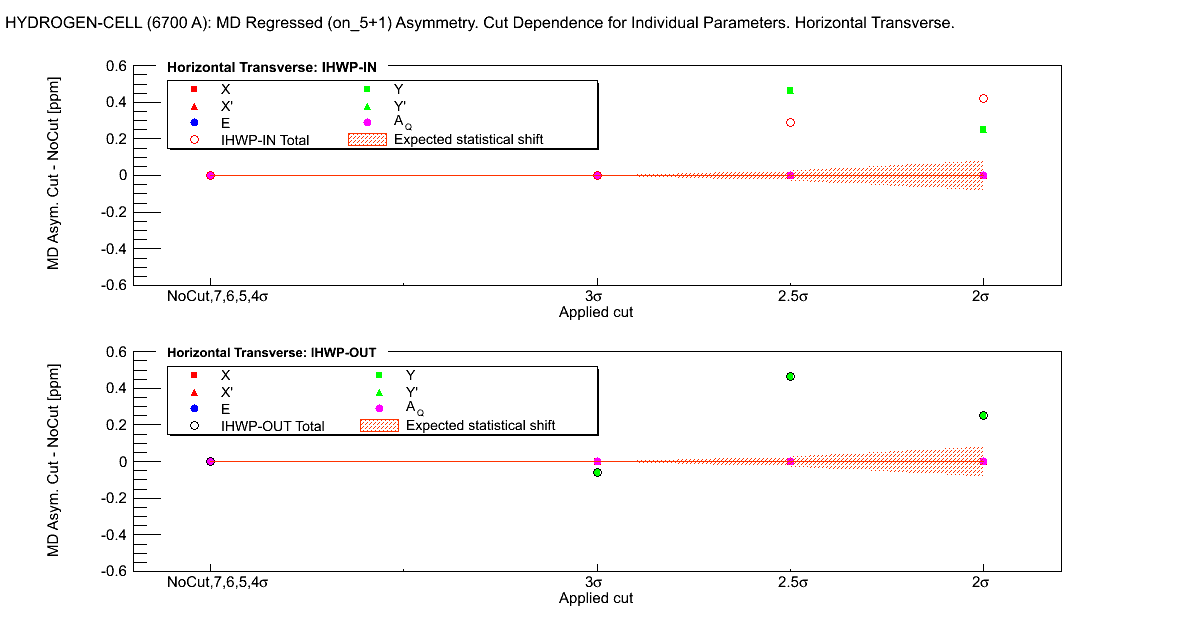
\includegraphics[width=15.0cm]{figures/cutDependence_LH2_h_individual}
	\end{center}
	\caption
%	[Cut dependence for horizontal transverse.]	
	{Cut dependence for horizontal transverse.}
	\label{fig:cutDependence_LH2_h_individual}
\end{figure}

\begin{figure}[!h]
	\begin{center}
	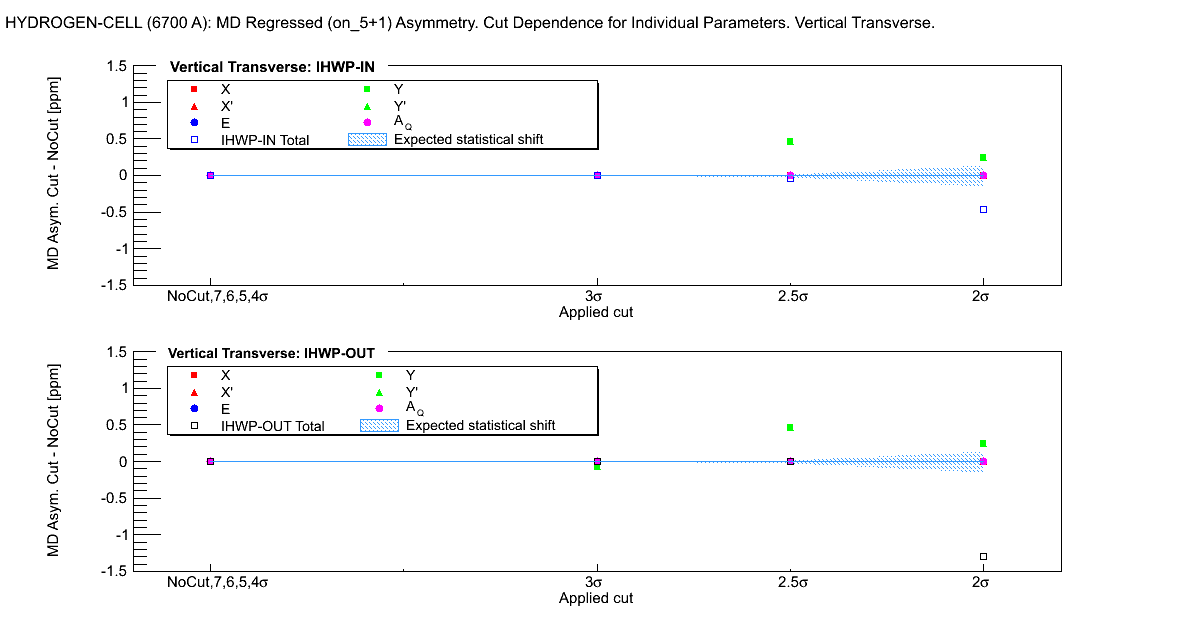
\includegraphics[width=15.0cm]{figures/cutDependence_LH2_v_individual}
	\end{center}
	\caption
%	[Cut dependence for vertical transverse.]
	{Cut dependence for vertical transverse.}
	\label{fig:cutDependence_LH2_v_individual}
\end{figure}



\begin{figure}[!h]
	\begin{center}
	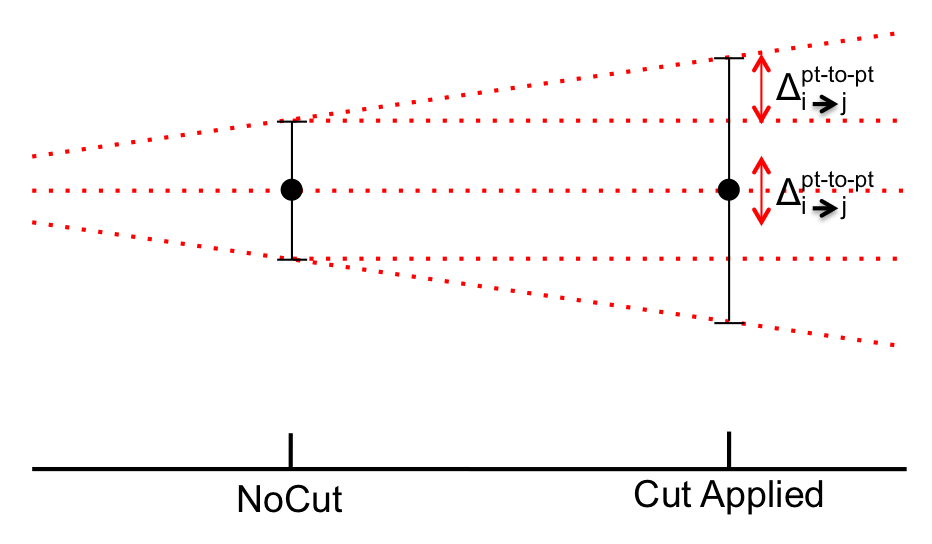
\includegraphics[width=8.0cm]{figures/cutDiagram}
	\end{center}
	\caption
%	[Cut dependence cartoon.]
	{Cut dependence cartoon.}
	\label{fig:CutDependenceCartoon.}
\end{figure}


\begin{table}[!h]
 \begin{center}
   \caption
%	[Cut dependence.]
	{Cut dependence.}
  \begin{tabular}{ c | c  c | c  c }
%    \hline
    \noalign{\hrule height 1pt}
    \multirow{3}{*}{Cut} 	&	\multicolumn{2}{c}{Horizontal} & \multicolumn{2}{|c}{Vertical} \\    
     \cline{2-5}
     & Allowed Statistical Shift & $\epsilon_{reg}^{H}$ Cut - NoCut & Allowed Statistical Shift & $\epsilon_{reg}^{V}$ Cut - NoCut\\
	 & [ppm] & [ppm] & [ppm] & [ppm] \\
%	\hline
    \noalign{\hrule height 1pt}
	7,6,5,4$\sigma$	&	0.000	&	0.000	&	0.000	&	0.000 \\
	3$\sigma$ 		&	0.001	&	0.024 	&	0.000	&	0.000 \\
	2.5$\sigma$ 		&	0.026	&	-0.064 &	0.021	&	-0.068 \\
	2$\sigma$ 		&	0.082	&	0.107 	&	0.142	&	0.367 \\
%	\hline
    \noalign{\hrule height 1pt}
   \end{tabular}
 \label{tab:cut_dependence}
 \end{center}
\end{table}


%%%%%%%%%%%%%%%%%%%%%%%%%%%%%%%%%%%%%%%%%%%%%%%%%%%%%%%%%%%%%
\section{Systematic Uncertainties for Other Transverse Datasets}
\label{Systematic Uncertainties for Other Transverse Datasets}

\begin{figure}[!h]
	\begin{center}
	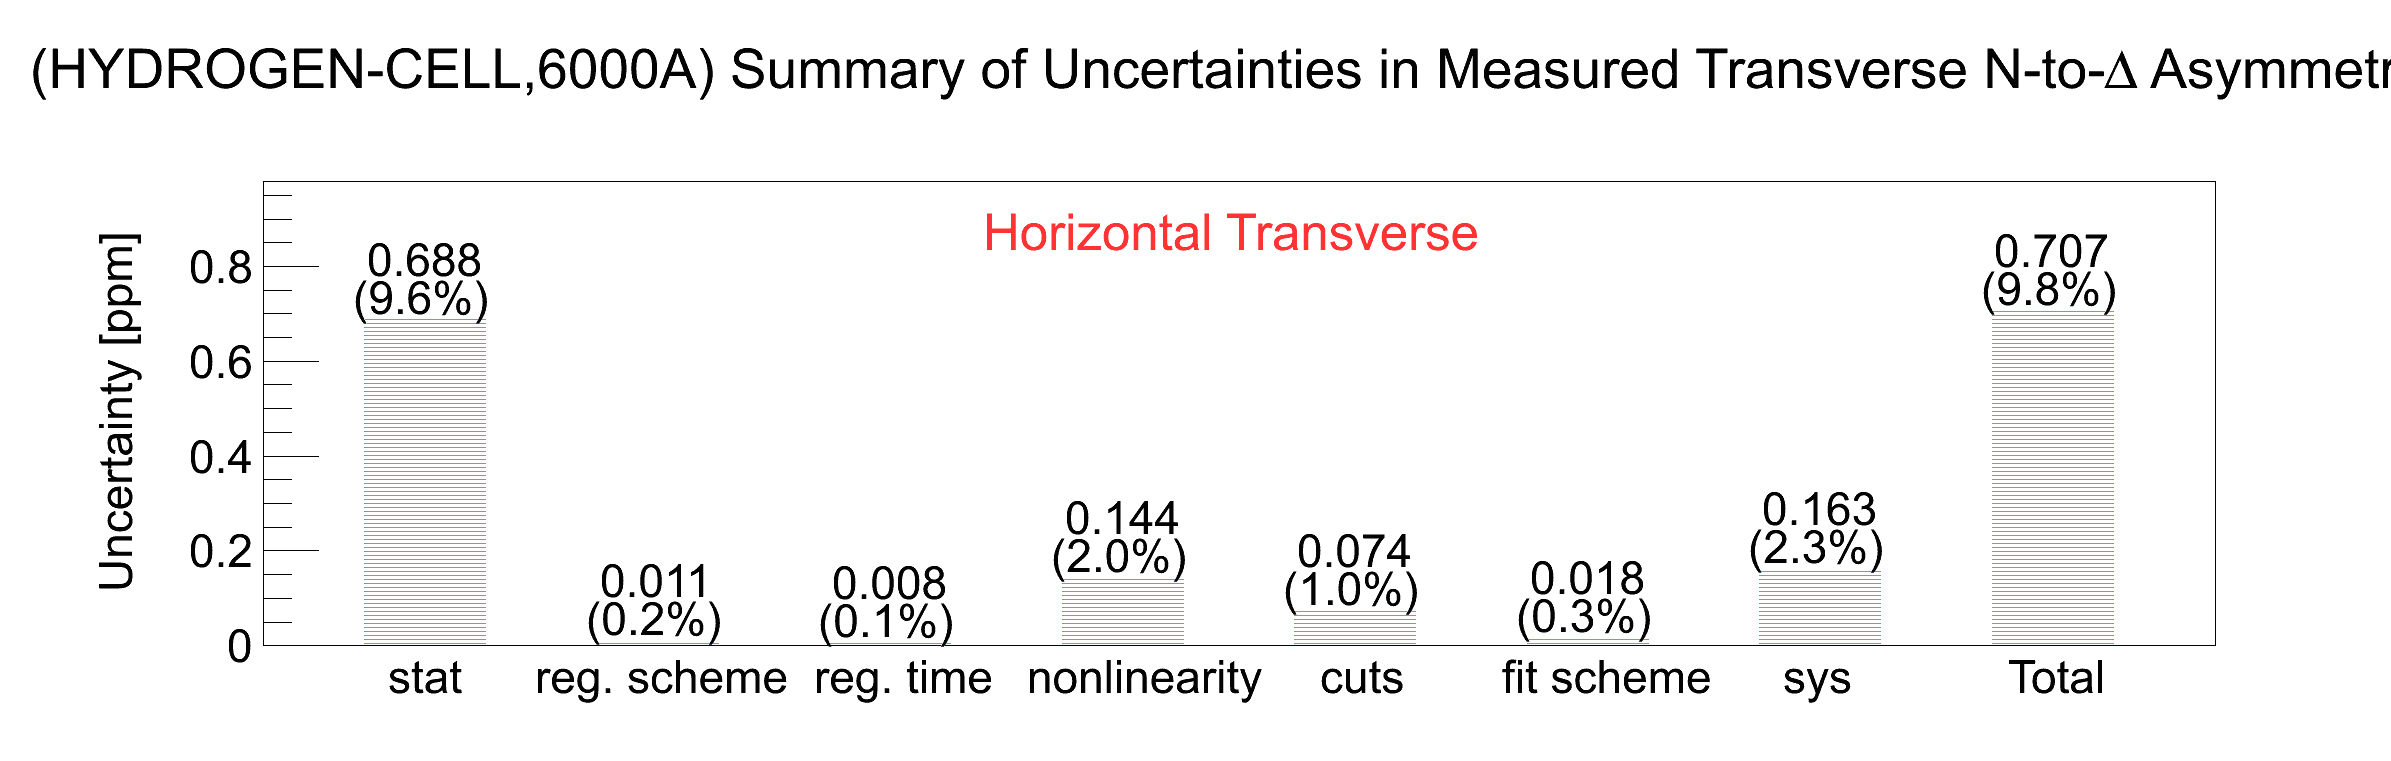
\includegraphics[width=15.0cm]{figures/errorChartLH2_6000A}
	\end{center}
	\caption
%	[Summary of uncertainties on measured asymmetry for transverse data set in LH$_{2}$ at QTor current 6000~A.]
	{Summary of uncertainties on measured asymmetry for transverse data set in LH$_{2}$ at QTor current 6000~A.}
	\label{fig:errorChartLH2_6000A}
\end{figure}

\begin{figure}[!h]
	\begin{center}
	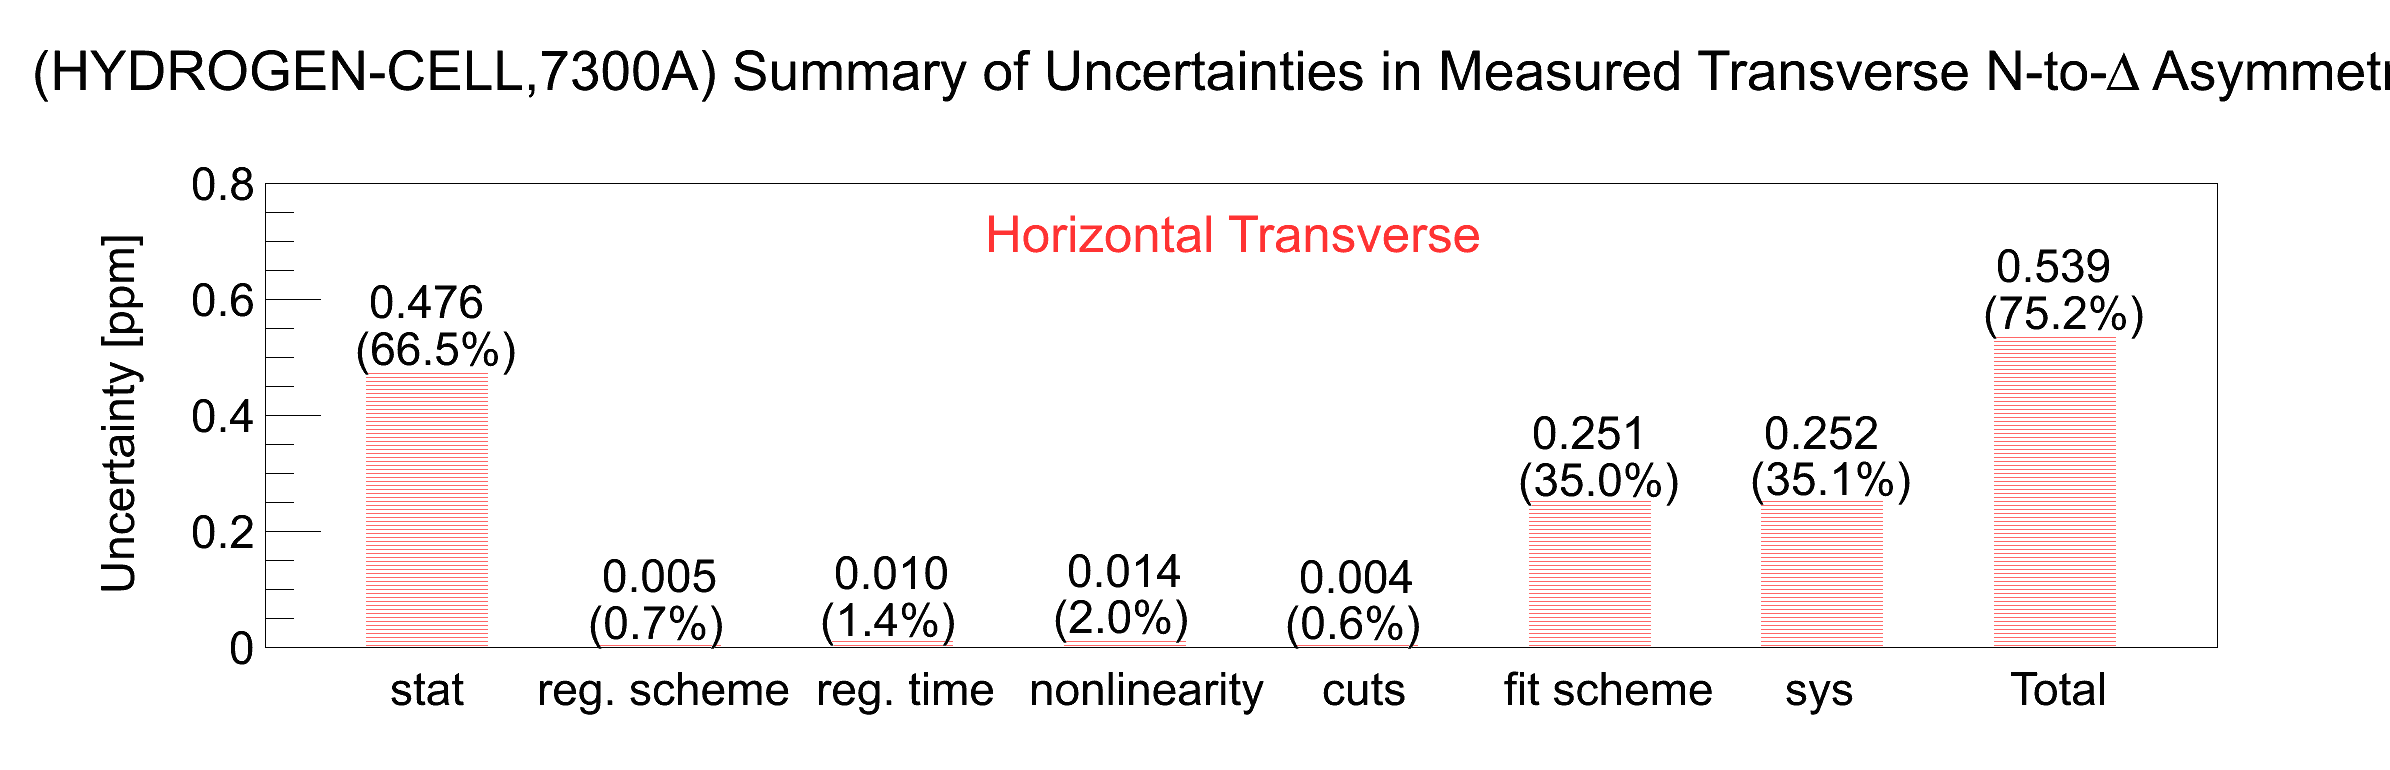
\includegraphics[width=15.0cm]{figures/errorChartLH2_7300A}
	\end{center}
	\caption
%	[Summary of uncertainties on measured asymmetry for transverse data set in LH$_{2}$ at QTor current 7300~A.]
	{Summary of uncertainties on measured asymmetry for transverse data set in LH$_{2}$ at QTor current 7300~A.}
	\label{fig:errorChartLH2_7300A}
\end{figure}


\begin{figure}[!h]
	\begin{center}
	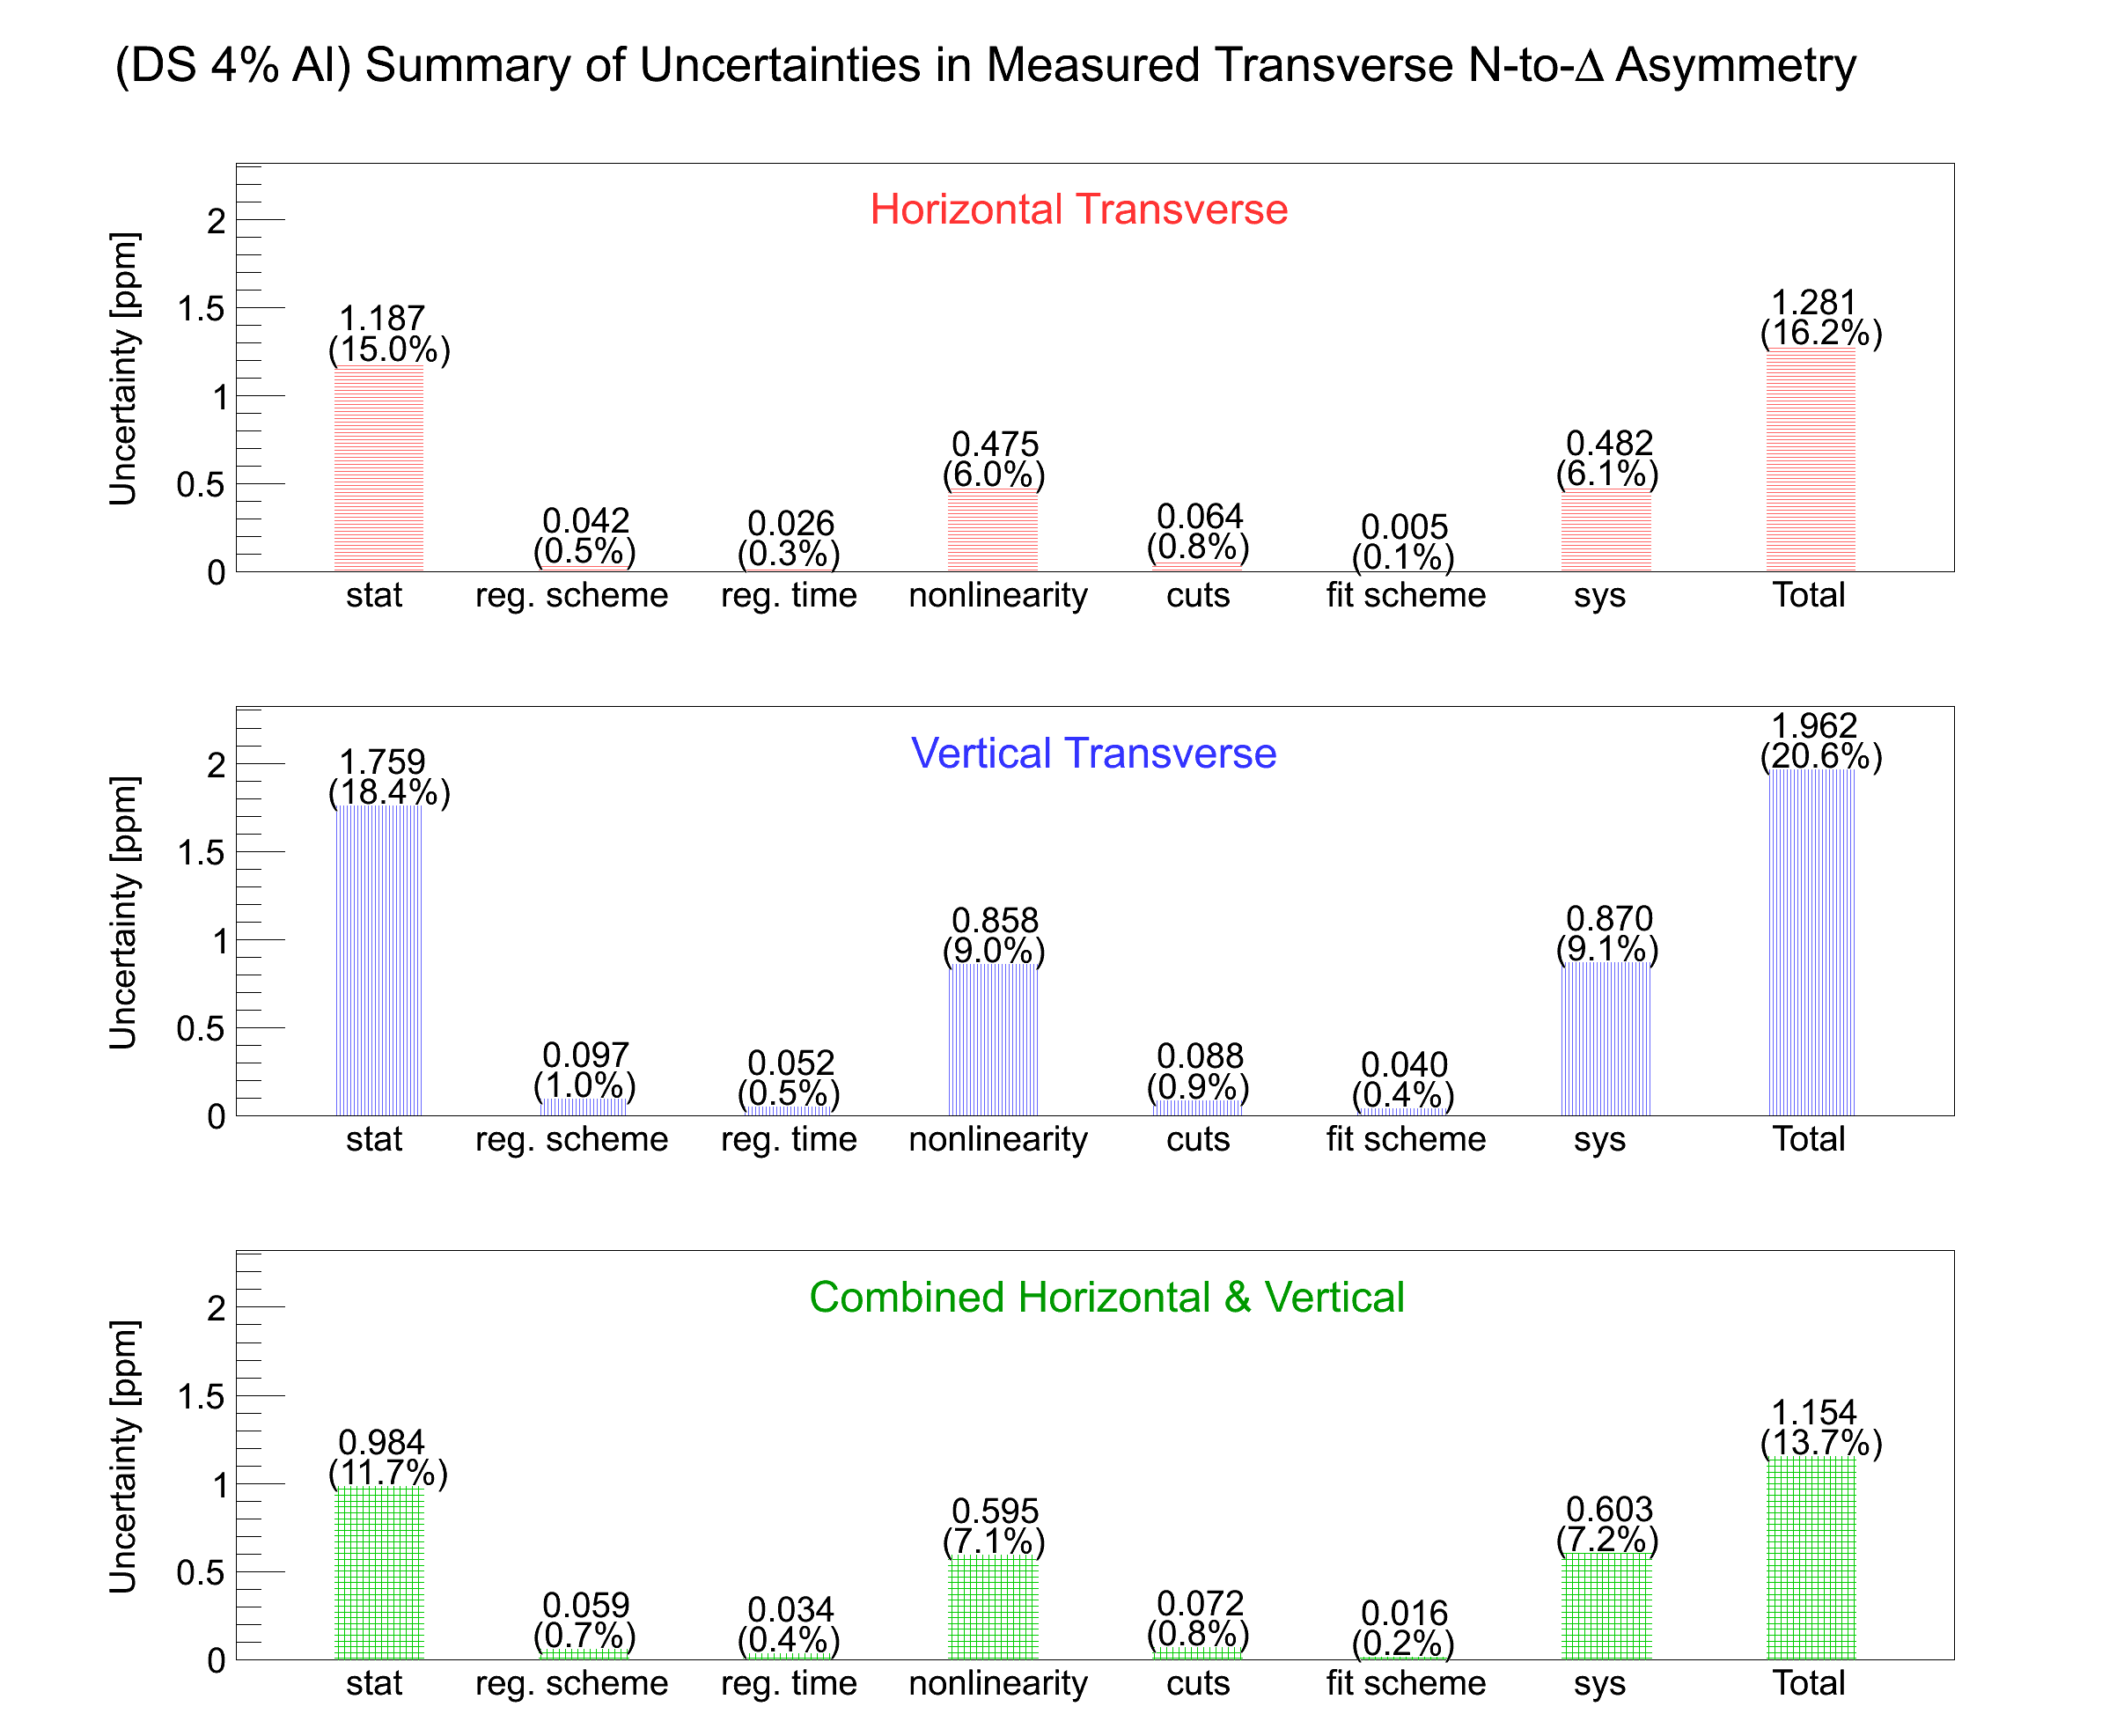
\includegraphics[width=15.0cm]{figures/errorChartAl_6700A}
	\end{center}
	\caption
%	[Summary of uncertainties on measured asymmetry for transverse data set in 4\% DS Al at QTor current 6700~A.]
	{Summary of uncertainties on measured asymmetry for transverse data set in 4\% DS Al at QTor current 6700~A.}
	\label{fig:errorChartAl_6700A}
\end{figure}

\begin{figure}[!h]
	\begin{center}
	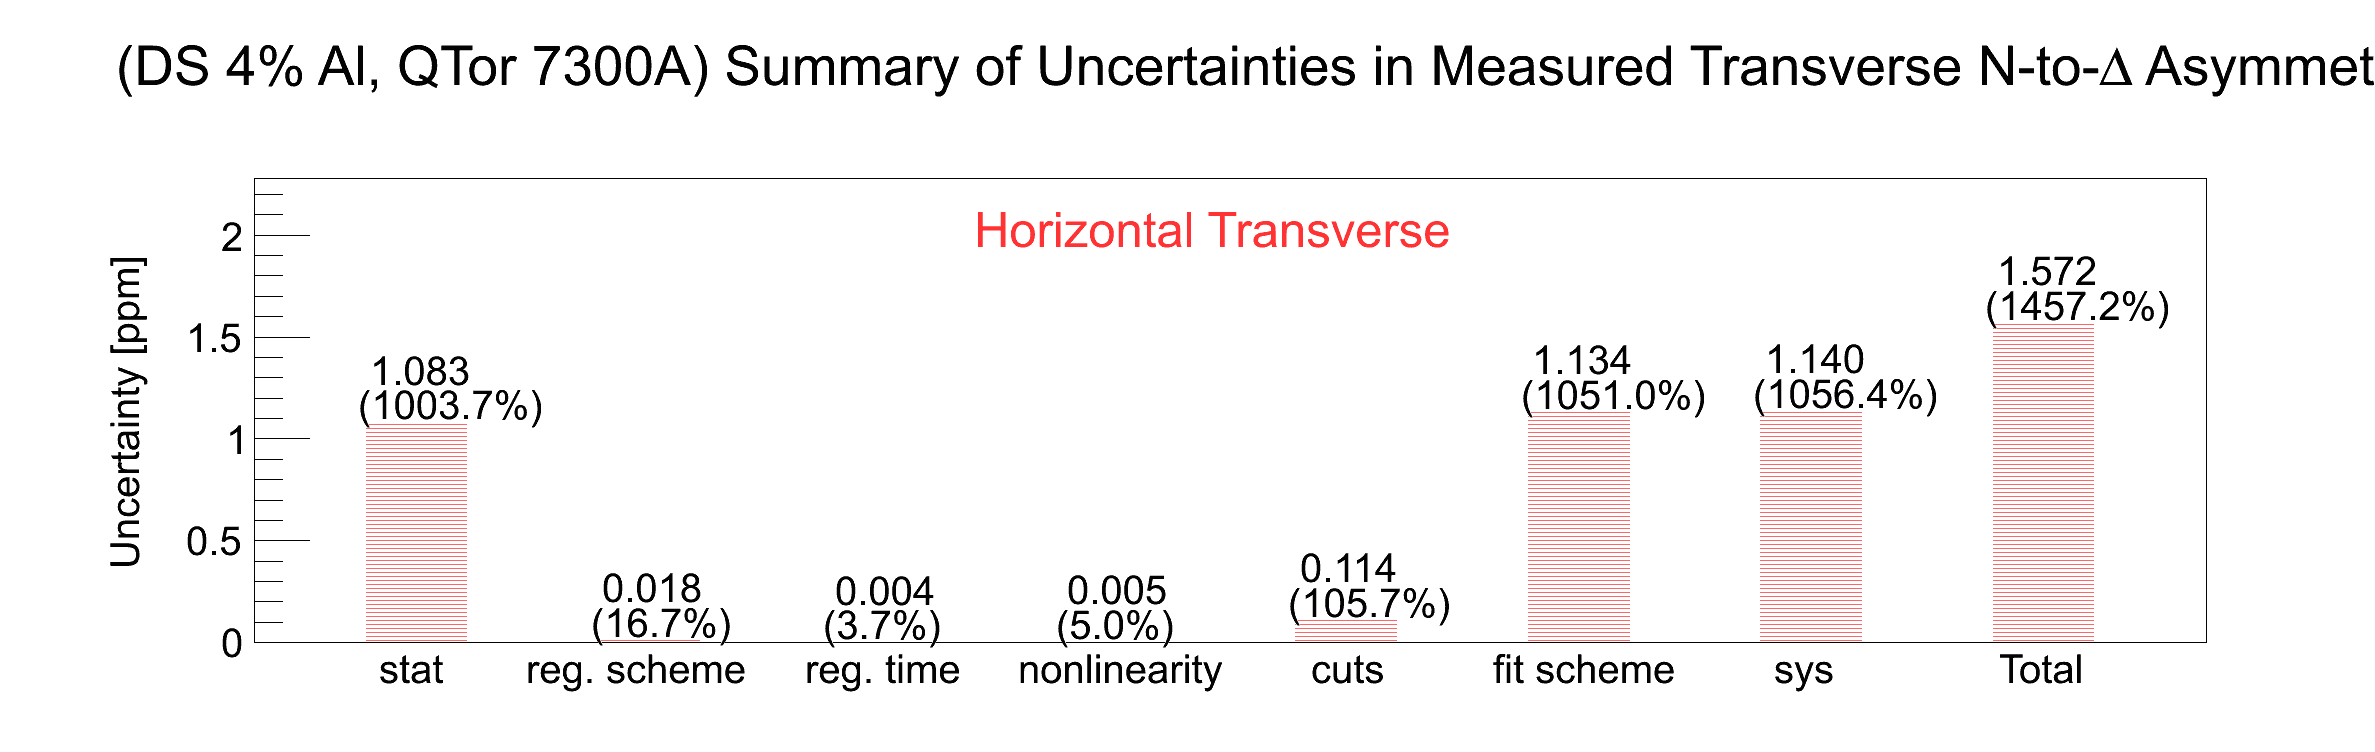
\includegraphics[width=15.0cm]{figures/errorChartAl_7300A}
	\end{center}
	\caption
%	[Summary of uncertainties on measured asymmetry for transverse data set in 4\% DS Al at QTor current 7300~A.]
	{Summary of uncertainties on measured asymmetry for transverse data set in 4\% DS Al at QTor current 7300~A.}
	\label{fig:errorChartAl_7300A}
\end{figure}

\begin{figure}[!h]
	\begin{center}
	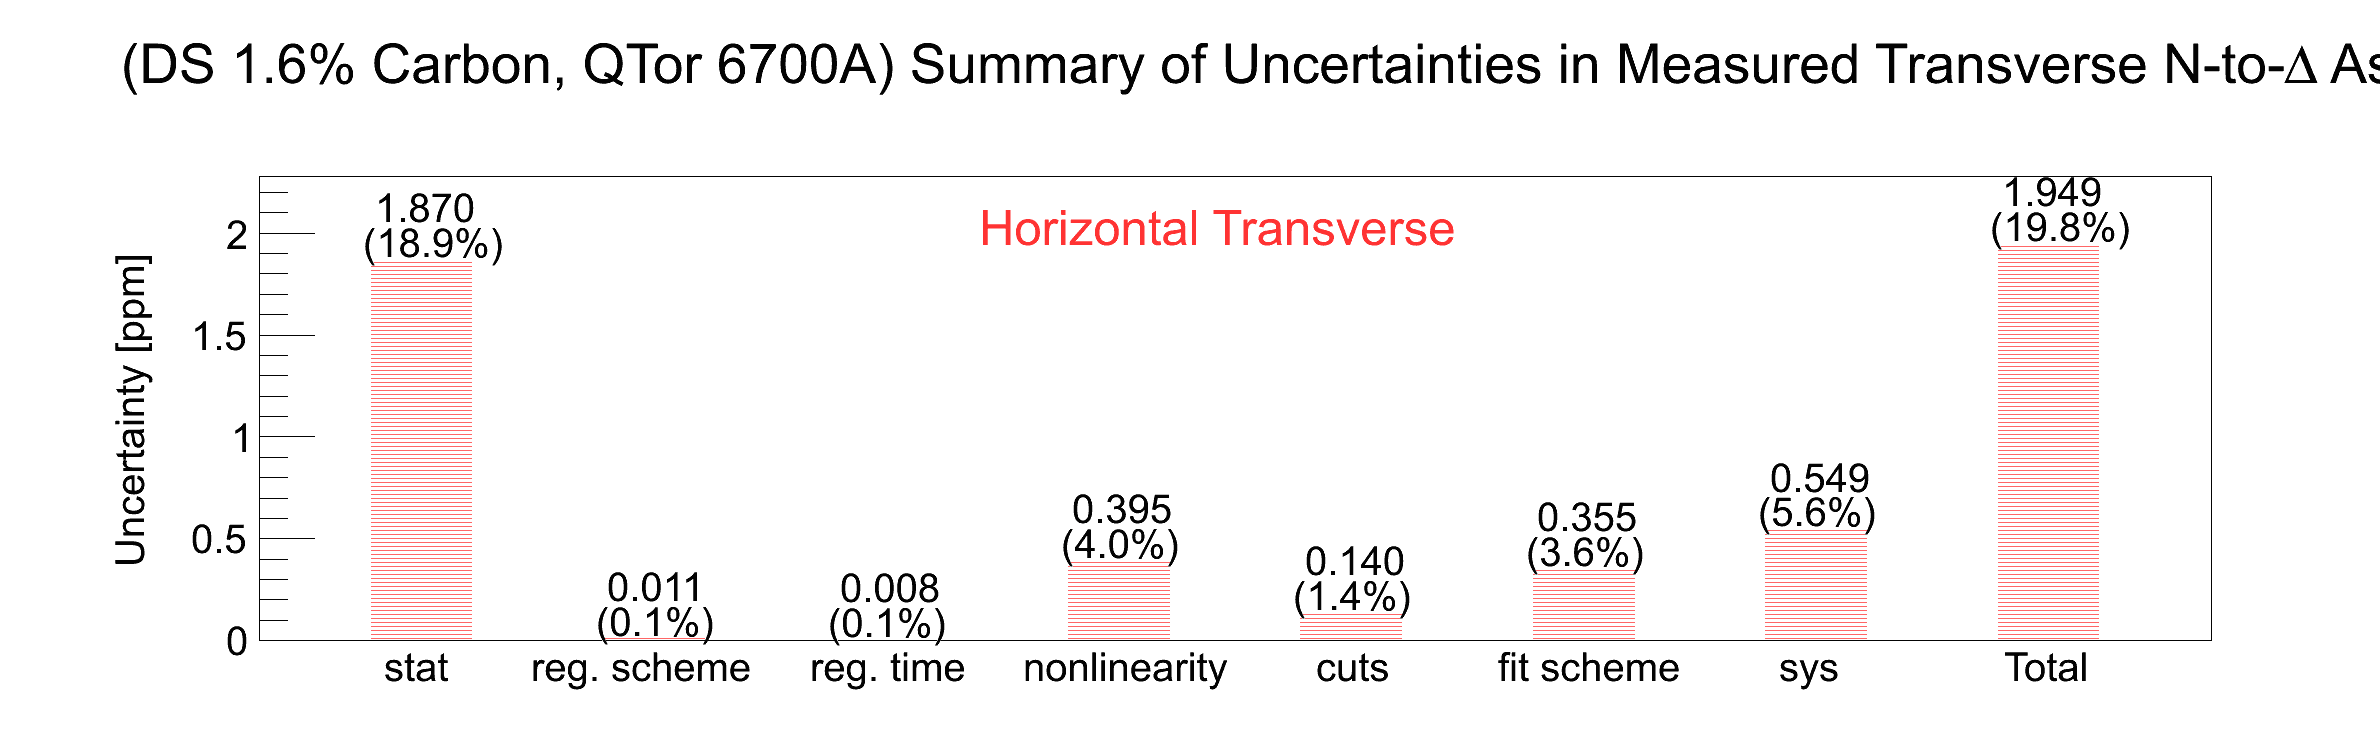
\includegraphics[width=15.0cm]{figures/errorChartC_6700A}
	\end{center}
	\caption
%	[Summary of uncertainties on measured asymmetry for transverse data set in Carbon at QTor current 6700~A.]
	{Summary of uncertainties on measured asymmetry for transverse data set in Carbon at QTor current 6700~A.}
	\label{fig:errorChartC_6700A}
\end{figure}



%%%%%%%%%%%%%%%%%%%%%%%%%%%%%%%%%%%%%%%%%%%%%%%%%%%%%%%%%%%%%
\section{Beamline Background Correction}
\label{Beamline Background Correction}

%Another correction accounts for scattering sources in the beam line ($BB$). The asymmetry ($A_{BB}$) was measured, along with its dilution ($f_{BB}$), by blocking two of the eight openings in the first of the three Pb collimators with tungsten. The measured asymmetry in the blocked octants detectors was correlated with different background detectors located outside the acceptance of the main detectors for scaling during the primary measurement, assuming a constant dilution~\cite{elog:kent_analysis782}. The variation of upstream luminosity monitor asymmetry with octant during longitudinal running can provide a good indication of the beamline scattering asymmetry. The maximum variation before and after the transverse data collection period (during longitudinal running) $\Delta A_{\rm USLumi}$ = 3.534~$\pm$~0.16~ppm (Figure~\ref{fig:USLumiSumAsymLongitudinal}) was used to estimate the beamline scattering asymmetry. A very simple postulate was considered: that measured main detector asymmetry has a background with a fixed fraction and an asymmetry that scales linearly with that measured in the background monitors and USLumis. The scale factor was measured directly, correlating the MD asymmetry to background asymmetries, and was estimated to be 0.0085~$\pm$~0.0016~\cite{elog:manolis_analysis1191} from longitudinal period. The signal drops by an order of magnitude lower for inelastic scattering compared to elastic, whereas beamline background remains similar. Hence an additional factor of 10 was multiplied to incorporate the signal drop. The beamline background does not depend on polarization and is not corrected for it. Then, asymmetry for beam line scattering is given by $A_{BB}$ = $\Delta A_{\rm USLumi}\times 0.085$ = 0.300~$\pm$~0.058~ppm. 

\begin{figure}[!h]
	\begin{center}
	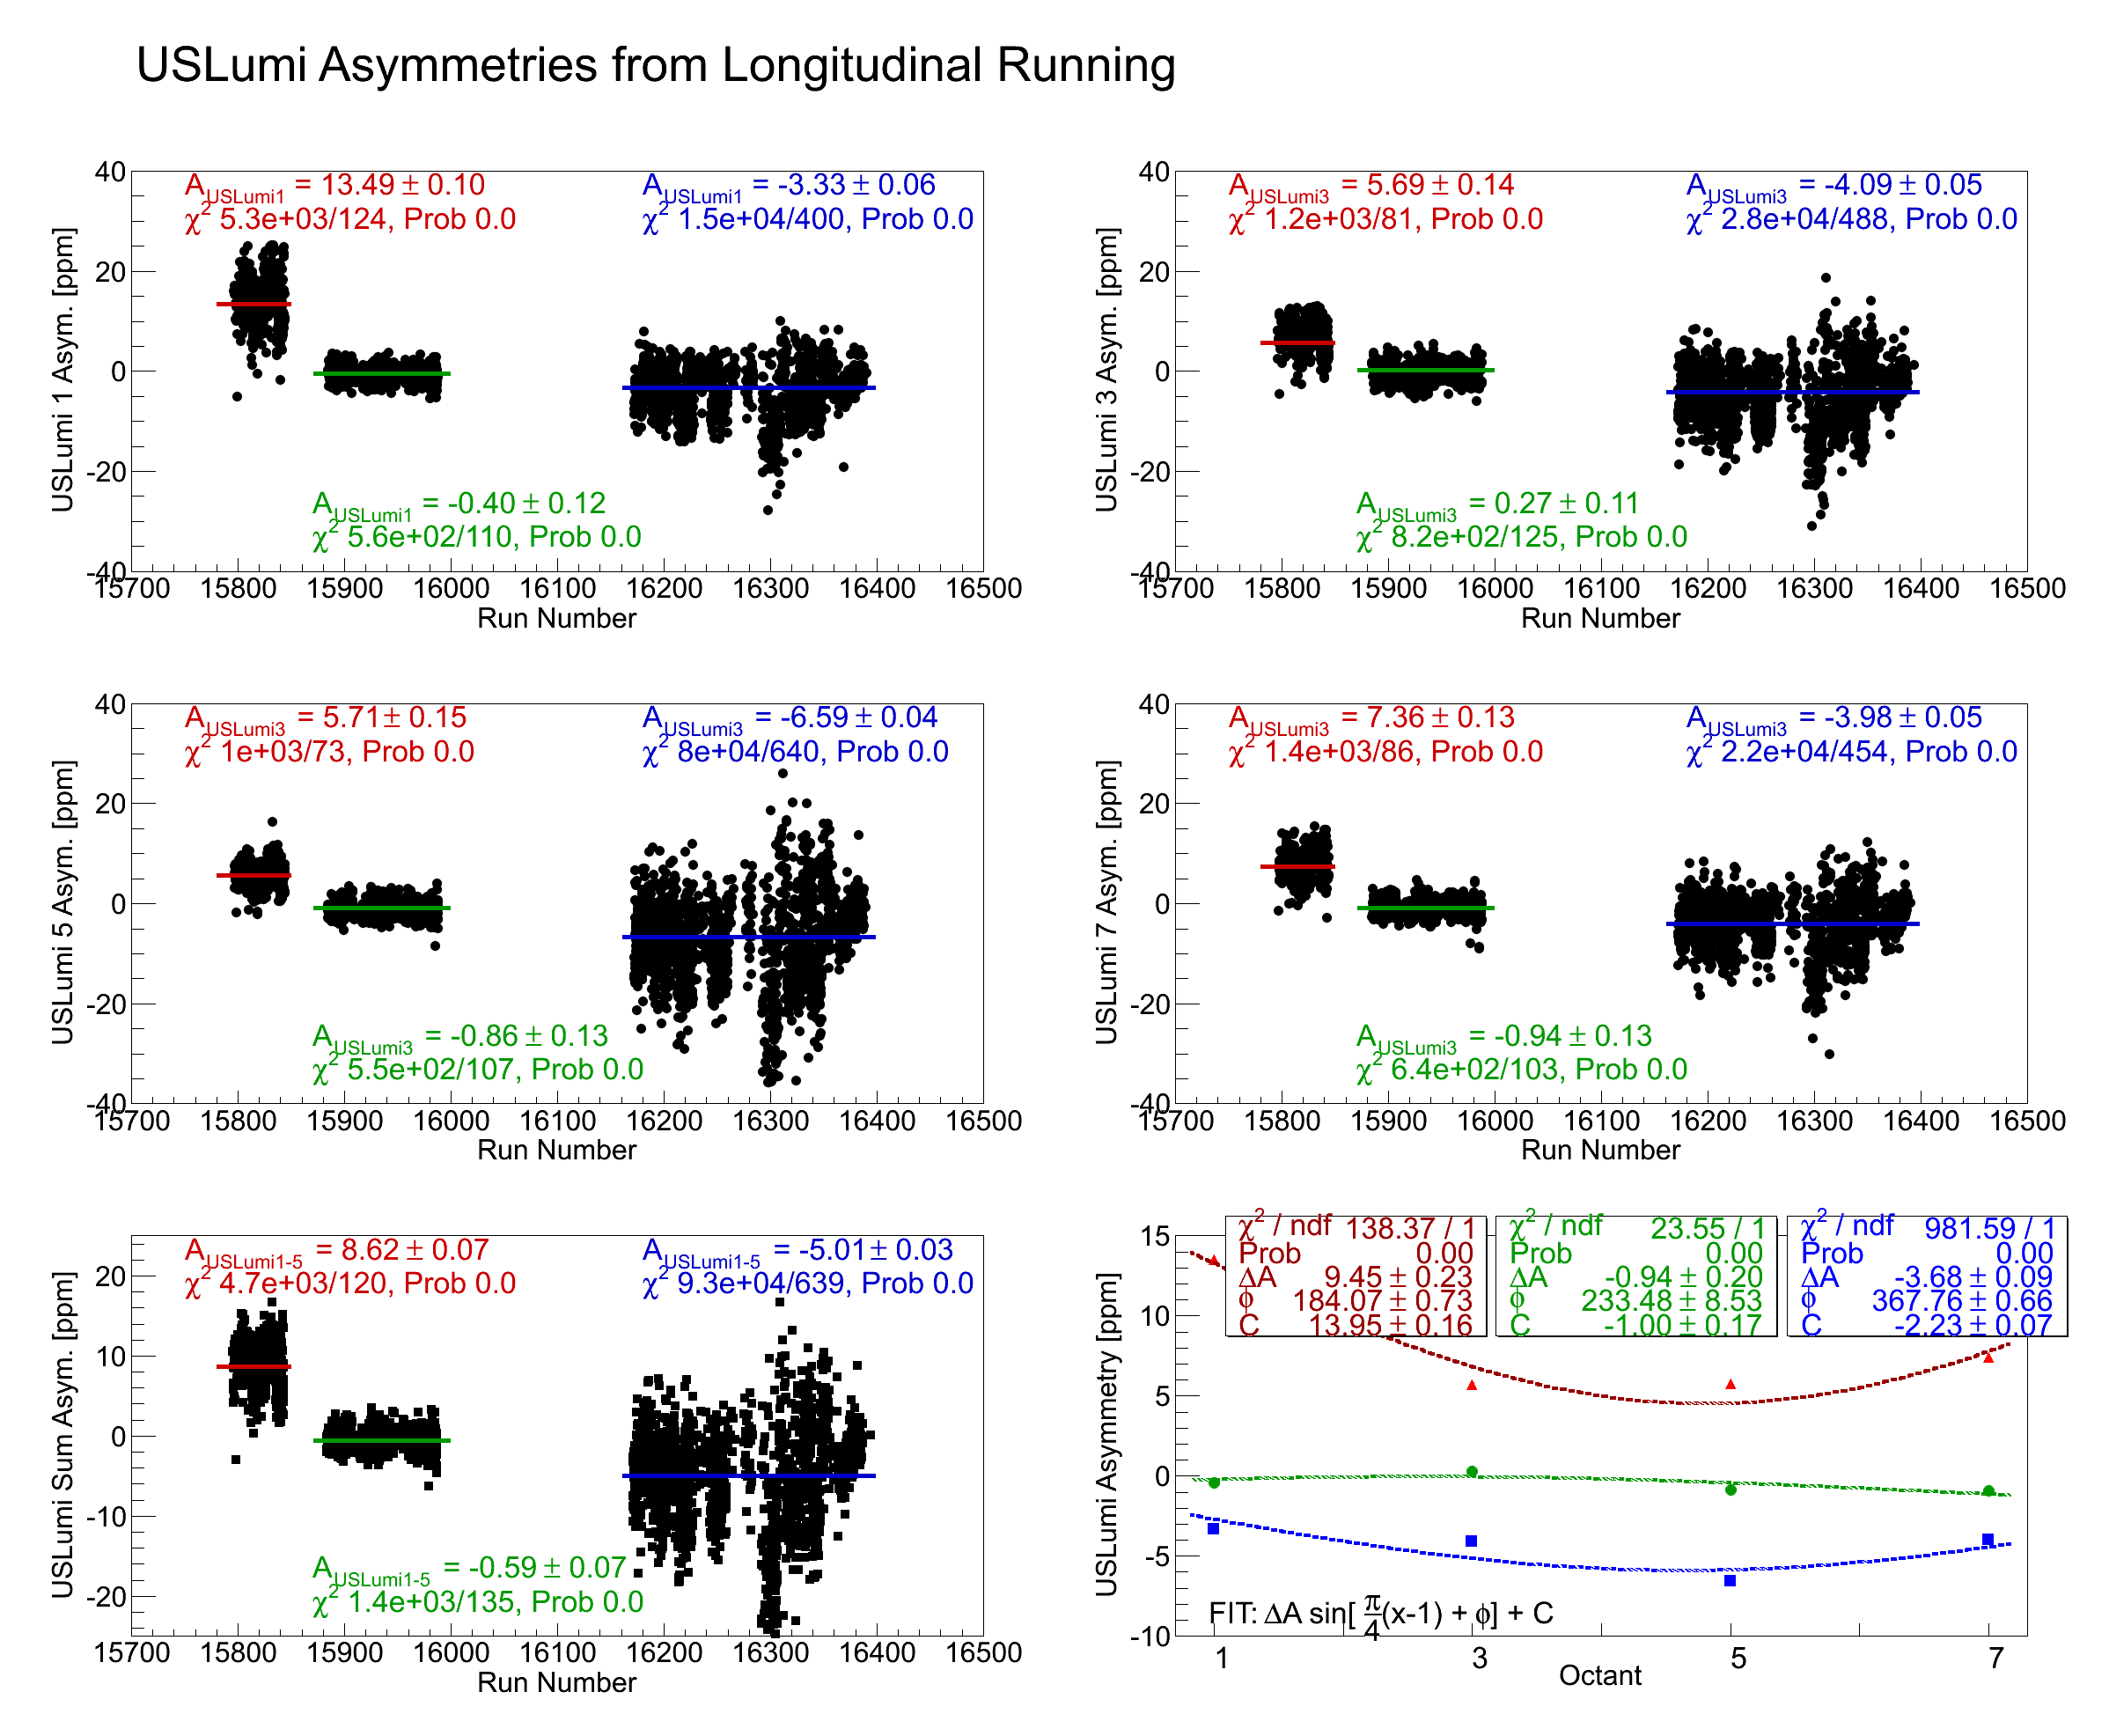
\includegraphics[width=15.0cm]{figures/USLumiSumAsymLongitudinal}
	\end{center}
	\caption
%	[Regressed ``5+1" USLumi asymmetries from longitudinal running.]
	{Regressed ``5+1" USLumi asymmetries longitudinal running for octant 1, 3, 5, and 7 are shown in panel 1-4. USLumi sum asymmetry is shown in panel 5. Each point is a runlet. The average asymmetries vs octant for each time period are shown in panel 6.}
	\label{fig:USLumiSumAsymLongitudinal}
\end{figure}
